% ==========================================
% BAB III ANALISIS DAN DESAIN
% ==========================================
\cleardoublepage
\chapter{ANALISIS DAN DESAIN}
\label{chap:III}

\section{Analisis Kebutuhan \textit{Framework}}
\label{sec:III.1}
\begin{figure}[htbp]
\centering
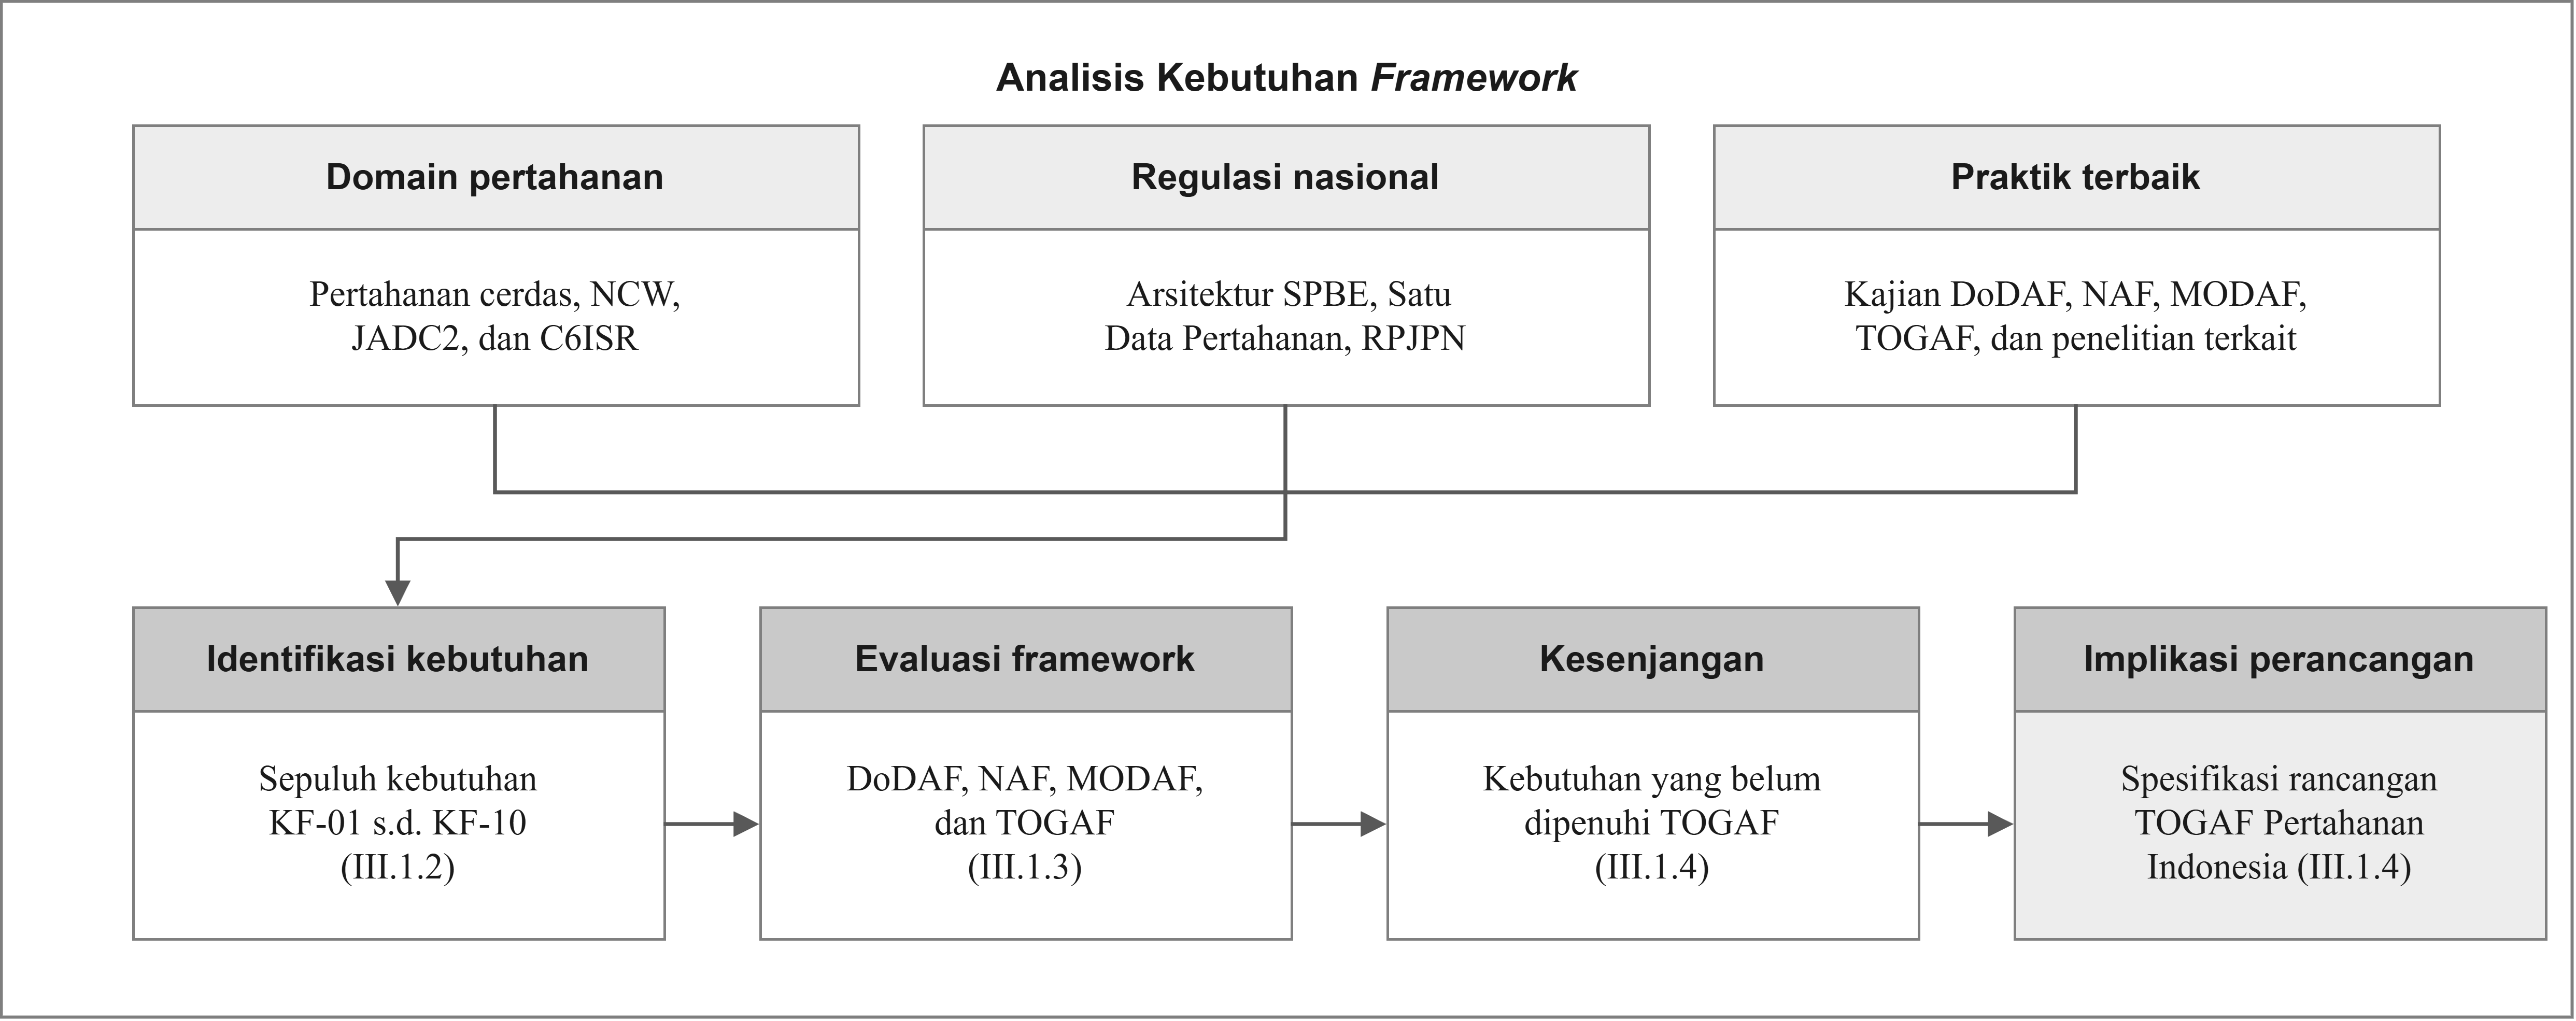
\includegraphics[width=1.00\linewidth,height=0.8\textheight,keepaspectratio]{images/Analisis_Kebutuhan_Framework.drawio.png}
\caption{Alur Analisis Kebutuhan Framework}
\label{fig:III.1}
\end{figure}

Analisis kebutuhan framework merumuskan kriteria yang harus dipenuhi \textit{framework} EA agar dapat digunakan untuk merancang arsitektur transformasi digital Kemhan RI. Analisis ini merupakan pelaksanaan tahap \textit{Defining the Objectives for a Solution} pada DSRM \cite{Peffers2007}. Alur analisis ditunjukkan pada Gambar~\ref{fig:III.1}.

Gambar~\ref{fig:III.1} menunjukkan bahwa kebutuhan framework dirumuskan dari tiga sumber, kemudian digunakan untuk mengevaluasi framework yang tersedia. Kebutuhan yang belum dipenuhi TOGAF menjadi kesenjangan, dan kesenjangan tersebut diterjemahkan menjadi implikasi perancangan bagi TOGAF Pertahanan Indonesia.

\subsection{Sumber dan Metode Perumusan Kebutuhan}
\label{sec:III.1.1}

Kebutuhan framework dirumuskan secara deduktif dari tiga sumber yang saling melengkapi, yaitu sebagai berikut.
\begin{enumerate}[label=\arabic*.]
\item Karakteristik domain pertahanan. Pertahanan cerdas menempatkan data sebagai aset strategis dan keunggulan informasi sebagai penentu keunggulan operasi. NCW dan JADC2 menuntut integrasi data, interoperabilitas, dan keamanan jaringan lintas domai, sedangkan C6ISR menuntut keterpaduan ISR, komando dan kendali, serta unsur penindak. Karakteristik ini membedakan domain pertahanan dari domain bisnis dan pemerintahan umum.
\item Regulasi nasional. Kemhan RI wajib menyelenggarakan SPBE \cite{Perpres95Tahun2018}, menyusun arsitektur SPBE yang berpedoman pada Arsitektur SPBE Nasional \cite{Perpres132Tahun2022}, serta mendukung percepatan transformasi digital \cite{Perpres82Tahun2023} dan arah pembangunan RPJPN 2025–2045 \cite{UU59Tahun2024}. Pada tingkat sektoral, kebutuhan diturunkan dari kebijakan Satu Data Pertahanan \cite{Permenhan1Tahun2023} dan Pedoman Pertahanan Siber \cite{Permenhan82Tahun2014}.
\item Praktik terbaik. Kajian DoDAF, NAF, MODAF, dan TOGAF menunjukkan kapabilitas yang dibutuhkan framework EA pertahanan.
\end{enumerate}

Ketiga sumber tersebut disintesiskan menjadi sepuluh kebutuhan framework dengan kode KF-01 hingga KF-10. Kode tersebut digunakan untuk menelusuri setiap kebutuhan pada evaluasi framework, perancangan modifikasi, verifikasi rancangan, dan evaluasi.

\subsection{Identifikasi Kebutuhan \textit{Framework}}
\label{sec:III.1.2}

Hasil sintesis berupa sepuluh kebutuhan framework disajikan pada Tabel~\ref{tab:III.1}.

\begingroup\small\setstretch{1.0}
\begin{longtable}{@{}>{\raggedright\arraybackslash\hspace{0pt}}p{0.104\linewidth}>{\raggedright\arraybackslash\hspace{0pt}}p{0.253\linewidth}>{\raggedright\arraybackslash\hspace{0pt}}p{0.414\linewidth}>{\raggedright\arraybackslash\hspace{0pt}}p{0.136\linewidth}@{}}
\caption{Kebutuhan Framework EA Kemhan RI}\label{tab:III.1}\\
\toprule
\textbf{Kode} & \textbf{Kebutuhan} & \textbf{Deskripsi} & \textbf{Sumber}\\
\midrule
\endfirsthead
\multicolumn{4}{@{}l}{\small\itshape \tablename\ \thetable{} (lanjutan)}\\
\toprule
\textbf{Kode} & \textbf{Kebutuhan} & \textbf{Deskripsi} & \textbf{Sumber}\\
\midrule
\endhead
\bottomrule
\endlastfoot
\centering\arraybackslash KF-01 & Metodologi pengembangan yang preskriptif dan iteratif & Menyediakan langkah pengembangan arsitektur secara bertahap. & \centering\arraybackslash P\\
\centering\arraybackslash KF-02 & Cakupan domain arsitektur inti & Mencakup domain bisnis, data, aplikasi, dan teknologi secara terpadu. & \centering\arraybackslash P, R\\
\centering\arraybackslash KF-03 & Akomodasi domain C6ISR & Mampu merancang kapabilitas C6ISR sebagai inti operasional pertahanan. & \centering\arraybackslash D\\
\centering\arraybackslash KF-04 & Keamanan siber sejak perancangan & Menanamkan keamanan sejak tahap perencanaan arsitektur (\textit{security by design}). & \centering\arraybackslash D, R\\
\centering\arraybackslash KF-05 & Interoperabilitas lintas entitas & Mengakomodasi pertukaran data antara Kemhan RI, Mabes TNI, ketiga matra, dan industri pertahanan. & \centering\arraybackslash D, R\\
\centering\arraybackslash KF-06 & Keterkaitan dengan doktrin dan strategi pertahanan & Menautkan arsitektur secara eksplisit dengan doktrin dan sasaran strategis pertahanan. & \centering\arraybackslash D\\
\centering\arraybackslash KF-07 & Keselarasan dengan regulasi nasional & Dapat diselaraskan dengan SPBE, Satu Data, dan RPJPN 2025–2045. & \centering\arraybackslash R\\
\centering\arraybackslash KF-08 & Fleksibilitas penyesuaian & Dapat disesuaikan (\textit{tailoring}) dengan karakteristik organisasi tanpa kehilangan integritas metodenya. & \centering\arraybackslash P\\
\centering\arraybackslash KF-09 & Tata kelola dan manajemen perubahan arsitektur & Menyediakan mekanisme tata kelola dan pengelolaan perubahan agar arsitektur tetap relevan. & \centering\arraybackslash P, R\\
\centering\arraybackslash KF-10 & Ketersediaan dan kematangan ekosistem & Tersedia terbuka untuk penggunaan akademik dan didukung ekosistem pengetahuan yang matang. & \centering\arraybackslash P\\
\end{longtable}
\endgroup

Keterangan: D = domain pertahanan; R = regulasi nasional; P = praktik terbaik.

Tabel~\ref{tab:III.1} menunjukkan bahwa kebutuhan framework terbagi dalam tiga kelompok. Kelompok metodologis, yaitu KF-01, KF-02, KF-08, KF-09, dan KF-10, berkaitan dengan cara arsitektur dikembangkan dan dikelola. Kelompok kontekstual pertahanan, yaitu KF-03 hingga KF-06, berkaitan dengan muatan khas pertahanan. KF-07 berkaitan dengan kewajiban Kemhan RI sebagai instansi pemerintah.

\subsection{Evaluasi Pemenuhan Kebutuhan oleh \textit{Framework} Saat Ini}
\label{sec:III.1.3}

Kesepuluh kebutuhan tersebut digunakan untuk mengevaluasi empat framework yang dibahas pada Bab II, yaitu DoDAF, NAF, MODAF, dan TOGAF. Penilaian didasarkan pada karakteristik framework pada Tabel~\ref{tab:II.4} dengan tiga tingkat pemenuhan, yaitu terpenuhi (T), terpenuhi sebagian (TS), dan tidak terpenuhi (TT). Hasil evaluasi disajikan pada Tabel~\ref{tab:III.2}.

\begingroup\small\setstretch{1.0}
\begin{longtable}{@{}>{\raggedright\arraybackslash\hspace{0pt}}p{0.097\linewidth}>{\raggedright\arraybackslash\hspace{0pt}}p{0.290\linewidth}>{\raggedright\arraybackslash\hspace{0pt}}p{0.115\linewidth}>{\raggedright\arraybackslash\hspace{0pt}}p{0.115\linewidth}>{\raggedright\arraybackslash\hspace{0pt}}p{0.115\linewidth}>{\raggedright\arraybackslash\hspace{0pt}}p{0.115\linewidth}@{}}
\caption{Evaluasi Pemenuhan Kebutuhan oleh Framework Saat Ini}\label{tab:III.2}\\
\toprule
\textbf{Kode} & \textbf{Kebutuhan} & \textbf{DoDAF} & \textbf{NAF} & \textbf{MODAF} & \textbf{TOGAF}\\
\midrule
\endfirsthead
\multicolumn{6}{@{}l}{\small\itshape \tablename\ \thetable{} (lanjutan)}\\
\toprule
\textbf{Kode} & \textbf{Kebutuhan} & \textbf{DoDAF} & \textbf{NAF} & \textbf{MODAF} & \textbf{TOGAF}\\
\midrule
\endhead
\bottomrule
\endlastfoot
\centering\arraybackslash KF-01 & Metodologi pengembangan yang preskriptif dan iteratif & \centering\arraybackslash TS & \centering\arraybackslash TS & \centering\arraybackslash TT & \centering\arraybackslash T\\
\centering\arraybackslash KF-02 & Cakupan domain arsitektur inti & \centering\arraybackslash T & \centering\arraybackslash T & \centering\arraybackslash T & \centering\arraybackslash T\\
\centering\arraybackslash KF-03 & Akomodasi domain C6ISR & \centering\arraybackslash T & \centering\arraybackslash T & \centering\arraybackslash T & \centering\arraybackslash TT\\
\centering\arraybackslash KF-04 & Keamanan siber sejak perancangan & \centering\arraybackslash TS & \centering\arraybackslash TS & \centering\arraybackslash TS & \centering\arraybackslash TS\\
\centering\arraybackslash KF-05 & Interoperabilitas lintas entitas & \centering\arraybackslash T & \centering\arraybackslash T & \centering\arraybackslash TS & \centering\arraybackslash TS\\
\centering\arraybackslash KF-06 & Keterkaitan dengan doktrin dan strategi pertahanan & \centering\arraybackslash T & \centering\arraybackslash T & \centering\arraybackslash T & \centering\arraybackslash TT\\
\centering\arraybackslash KF-07 & Keselarasan dengan regulasi nasional & \centering\arraybackslash TS & \centering\arraybackslash TS & \centering\arraybackslash TS & \centering\arraybackslash T\\
\centering\arraybackslash KF-08 & Fleksibilitas penyesuaian & \centering\arraybackslash TS & \centering\arraybackslash TS & \centering\arraybackslash TT & \centering\arraybackslash T\\
\centering\arraybackslash KF-09 & Tata kelola dan manajemen perubahan arsitektur & \centering\arraybackslash TS & \centering\arraybackslash TS & \centering\arraybackslash TS & \centering\arraybackslash T\\
\centering\arraybackslash KF-10 & Ketersediaan dan kematangan ekosistem & \centering\arraybackslash TS & \centering\arraybackslash TS & \centering\arraybackslash TT & \centering\arraybackslash T\\
\end{longtable}
\endgroup

Keterangan: T = terpenuhi; TS = terpenuhi sebagian; TT = tidak terpenuhi.

Tabel~\ref{tab:III.2} menunjukkan bahwa DoDAF, NAF, dan MODAF unggul pada kebutuhan kontekstual pertahanan, yaitu KF-03, KF-05, dan KF-06, karena ketiganya berakar pada C4ISR Architecture Framework. Namun, ketiganya lemah pada kebutuhan metodologis karena menekankan apa yang harus dideskripsikan, sedangkan langkah pengembangannya bersifat umum. NAF telah memiliki metodologi, tetapi dirancang untuk interoperabilitas di lingkungan NATO \cite{NAFv41}.

Sebaliknya, TOGAF memenuhi seluruh kebutuhan metodologis dan KF-07. ADM menyediakan langkah pengembangan yang iteratif dengan \textit{Requirements Management} di pusat siklus, mewajibkan penyesuaian sejak \textit{Fase Preliminary}, dan memiliki domain yang berpadanan dengan SPBE (Tabel~\ref{tab:II.2}). Kelemahan TOGAF terletak pada kebutuhan kontekstual pertahanan. KF-03 dan KF-06 tidak terpenuhi, sedangkan KF-04 dan KF-05 hanya terpenuhi sebagian. KF-04 terpenuhi sebagian karena \textit{The Open Group} telah menyediakan panduan integrasi risiko dan keamanan ke dalam ADM, tetapi keamanan masih diperlakukan sebagai \textit{concern} lintas domain \cite{TOGAFRiskSecurity}. KF-05 terpenuhi sebagian karena interoperabilitas dalam TOGAF bersifat umum dan belum diarahkan pada banyak entitas dengan struktur komando lintas matra.

\subsection{Kesenjangan Kebutuhan dan Implikasi Perancangan}
\label{sec:III.1.4}

Hasil evaluasi menunjukkan bahwa tidak ada \textit{framework} yang memenuhi seluruh kebutuhan. \textit{Framework} pertahanan memenuhi kebutuhan kontekstual, tetapi lemah dalam metodologi pengembangan. Sebaliknya, TOGAF kuat dalam metodologi, tetapi tidak memuat konteks pertahanan. Oleh karena itu, kesenjangan tersebut tidak dapat diselesaikan hanya dengan memilih salah satu \textit{framework}, melainkan dengan memodifikasi \textit{framework} yang memiliki fondasi metodologis terkuat.

TOGAF dipilih sebagai dasar modifikasi karena dua alasan. Pertama, kebutuhan yang belum dipenuhi TOGAF lebih sedikit dan bersifat aditif, sehingga dapat ditutup dengan menambahkan muatan pertahanan. Kedua, TOGAF mewajibkan penyesuaian sejak \textit{Fase Preliminary}, sehingga muatan tersebut dapat ditambahkan tanpa merusak integritas metodenya. NAF tidak dipilih sebagai framework utama karena berorientasi pada lingkungan NATO dan memerlukan pemetaan ulang terhadap domain Arsitektur SPBE, sedangkan penggunaan NAF dan TOGAF secara paralel akan menggandakan artefak. Meskipun demikian, \textit{concern} kapabilitas dan interoperabilitas pada NAF tetap digunakan sebagai salah satu rujukan muatan \textit{Fase C6ISR Architecture}.

Kesenjangan pada TOGAF beserta implikasinya terhadap perancangan dirangkum pada Tabel~\ref{tab:III.3}.

\begingroup\small\setstretch{1.0}
\begin{longtable}{@{}>{\raggedright\arraybackslash\hspace{0pt}}p{0.107\linewidth}>{\raggedright\arraybackslash\hspace{0pt}}p{0.401\linewidth}>{\raggedright\arraybackslash\hspace{0pt}}p{0.428\linewidth}@{}}
\caption{Kesenjangan pada TOGAF dan Implikasi Perancangan}\label{tab:III.3}\\
\toprule
\textbf{Kode} & \textbf{Kesenjangan pada TOGAF} & \textbf{Implikasi Perancangan}\\
\midrule
\endfirsthead
\multicolumn{3}{@{}l}{\small\itshape \tablename\ \thetable{} (lanjutan)}\\
\toprule
\textbf{Kode} & \textbf{Kesenjangan pada TOGAF} & \textbf{Implikasi Perancangan}\\
\midrule
\endhead
\bottomrule
\endlastfoot
\centering\arraybackslash KF-03 & Tidak tersedia domain arsitektur untuk kapabilitas C6ISR. & Penambahan \textit{Fase C6ISR Architecture} (+) sebagai domain arsitektur tersendiri dalam siklus ADM.\\
\centering\arraybackslash KF-04 & Keamanan diperlakukan sebagai \textit{concern} lintas domain tanpa prinsip yang mengikat. & Penetapan \textit{security by design} sebagai prinsip arsitektur dan penguatan arsitektur keamanan pada \textit{Fase Technology Architecture} (Δ).\\
\centering\arraybackslash KF-05 & Interoperabilitas belum diarahkan pada banyak entitas dengan struktur komando lintas matra. & Penetapan interoperabilitas sebagai prinsip arsitektur serta standar integrasi pada \textit{Fase Business Architecture} dan \textit{Information Systems Architecture} (Δ).\\
\centering\arraybackslash KF-06 & Tidak ada penautan eksplisit antara arsitektur dan doktrin serta strategi pertahanan. & Penambahan masukan doktrin dan strategi pertahanan pada \textit{Fase Preliminary} dan \textit{Architecture Vision} (Δ).\\
\end{longtable}
\endgroup

Keempat implikasi tersebut menjadi spesifikasi rancangan bagi TOGAF Pertahanan Indonesia. KF-03 dipenuhi melalui penambahan fase, sedangkan KF-04, KF-05, dan KF-06 dipenuhi melalui penyesuaian muatan fase yang sudah ada dan prinsip arsitektur.

\section{Desain Modifikasi TOGAF Berbasis C6ISR}
\label{sec:III.2}

Subbab ini menerjemahkan implikasi perancangan pada Tabel~\ref{tab:III.3} menjadi desain modifikasi TOGAF.

\subsection{Strategi Modifikasi TOGAF ADM}
\label{sec:III.2.1}

Modifikasi dilakukan melalui penyesuaian yang disediakan TOGAF, yaitu penyesuaian terminologi, proses, dan konten. Strategi modifikasi terdiri atas tiga langkah berikut.
\begin{enumerate}[label=\arabic*.]
\item Mempertahankan struktur siklus ADM dan menempatkan \textit{Requirements Management} tetap di pusat siklus agar integritas metode TOGAF terjaga.
\item Menambahkan satu fase baru (+) untuk kesenjangan yang tidak dapat ditampung oleh fase yang ada, yaitu KF-03 melalui \textit{Fase C6ISR Architecture}.
\item Menyesuaikan muatan fase yang sudah ada (Δ) untuk kesenjangan yang dapat ditampung oleh fase tersebut, yaitu KF-04, KF-05, dan KF-06.
\end{enumerate}

Hasil modifikasi tersebut ditunjukkan pada Gambar~\ref{fig:III.2}.
\begin{figure}[htbp]
\centering
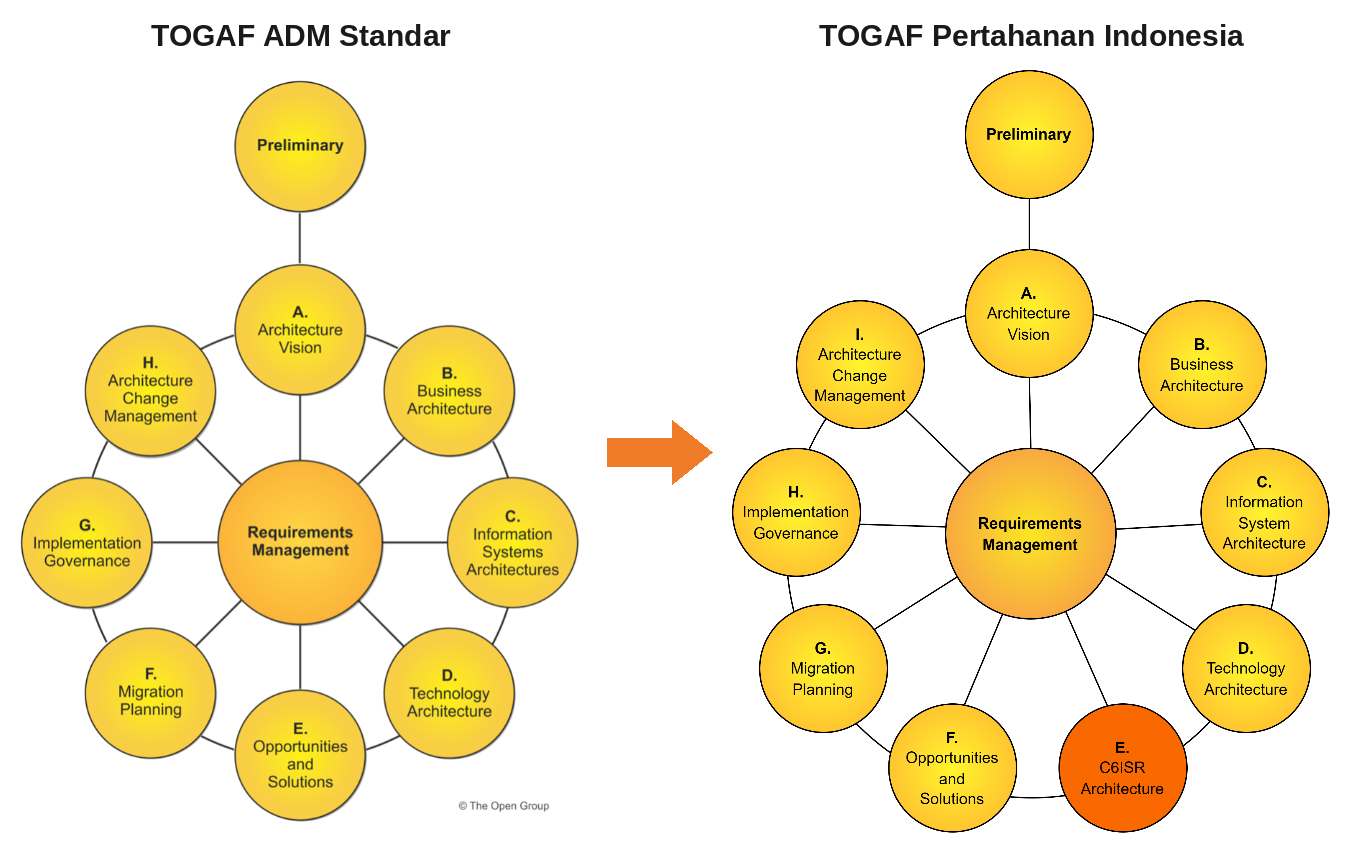
\includegraphics[width=1.00\linewidth,height=0.8\textheight,keepaspectratio]{images/Perbandingan TOGAF ADM Standar dan TOGAF Pertahanan Indonesia.png}
\caption{Perbandingan TOGAF ADM Standar dan TOGAF Pertahanan Indonesia}
\label{fig:III.2}
\end{figure}

Gambar~\ref{fig:III.2} menunjukkan bahwa \textit{Fase C6ISR Architecture} ditempatkan sebagai Fase E, setelah \textit{Fase Technology Architecture} dan sebelum \textit{Fase Opportunities \& Solutions}. Penempatan ini dipilih karena \textit{Fase C6ISR Architecture} membutuhkan keluaran arsitektur bisnis, data, aplikasi, teknologi, dan keamanan sebagai fondasinya, sedangkan kesenjangannya perlu dikonsolidasikan bersama domain lain pada \textit{Fase Opportunities \& Solutions}. Akibatnya, fase-fase berikutnya bergeser menjadi Fase F hingga Fase I. Jenis modifikasi pada setiap fase dirangkum pada Tabel~\ref{tab:III.4}.

\begingroup\small\setstretch{1.0}
\begin{longtable}{@{}>{\raggedright\arraybackslash\hspace{0pt}}p{0.291\linewidth}>{\raggedright\arraybackslash\hspace{0pt}}p{0.078\linewidth}>{\raggedright\arraybackslash\hspace{0pt}}p{0.389\linewidth}>{\raggedright\arraybackslash\hspace{0pt}}p{0.149\linewidth}@{}}
\caption{Jenis Modifikasi pada Setiap Fase}\label{tab:III.4}\\
\toprule
\textbf{Fase} & \textbf{Jenis} & \textbf{Muatan Modifikasi} & \textbf{Kebutuhan}\\
\midrule
\endfirsthead
\multicolumn{4}{@{}l}{\small\itshape \tablename\ \thetable{} (lanjutan)}\\
\toprule
\textbf{Fase} & \textbf{Jenis} & \textbf{Muatan Modifikasi} & \textbf{Kebutuhan}\\
\midrule
\endhead
\bottomrule
\endlastfoot
\textit{Preliminary} & \centering\arraybackslash Δ & Masukan doktrin, strategi pertahanan, dan regulasi nasional; penetapan sembilan prinsip arsitektur. & \centering\arraybackslash KF-04 s.d.\newline KF-07\\
A. \textit{Architecture Vision} & \centering\arraybackslash Δ & Visi arsitektur yang berorientasi pada pertahanan cerdas; pendorong, kendala, dan risiko transformasi pertahanan. & \centering\arraybackslash KF-06\\
B. \textit{Business Architecture} & \centering\arraybackslash Δ & Kapabilitas dan proses bisnis yang mendukung komando-kendali serta kolaborasi lintas satuan. & \centering\arraybackslash KF-05\\
C. \textit{Information Systems Architecture} & \centering\arraybackslash Δ & Klasifikasi kerahasiaan data serta standar integrasi data dan aplikasi lintas entitas. & \centering\arraybackslash KF-04,\newline KF-05\\
D. \textit{Technology Architecture} & \centering\arraybackslash Δ & Prinsip dan standar teknologi serta lapisan arsitektur keamanan. & \centering\arraybackslash KF-04\\
E. \textit{C6ISR Architecture} & \centering\arraybackslash + & Arsitektur kapabilitas C6ISR yang mengintegrasikan ISR, komando-kendali, dan unsur penindak. & \centering\arraybackslash KF-03\\
F. Opportunities \& Solutions & \centering\arraybackslash – & Mengikuti TOGAF ADM standar dengan tambahan masukan kesenjangan dari \textit{Fase C6ISR Architecture}. & \centering\arraybackslash –\\
G. Migration Planning & \centering\arraybackslash – & Mengikuti TOGAF ADM standar dengan tambahan paket pekerjaan dari \textit{Fase C6ISR Architecture}. & \centering\arraybackslash –\\
H. Implementation Governance & \centering\arraybackslash – & Mengikuti TOGAF ADM standar. & \centering\arraybackslash –\\
I. Architecture Change Management & \centering\arraybackslash – & Mengikuti TOGAF ADM standar. & \centering\arraybackslash –\\
\end{longtable}
\endgroup

Keterangan: Δ = muatan fase disesuaikan; + = fase baru; – = mengikuti TOGAF ADM standar.

Tabel~\ref{tab:III.4} menunjukkan bahwa modifikasi terkonsentrasi pada enam fase pertama. Empat fase terakhir dipertahankan karena telah memadai untuk mewujudkan, mengendalikan, dan memelihara arsitektur.

\subsection{Pemetaan Unsur C6ISR terhadap Fase TOGAF}
\label{sec:III.2.2}

Pemetaan unsur C6ISR terhadap fase TOGAF dilakukan untuk menentukan muatan yang dapat ditampung oleh fase standar dan muatan yang membutuhkan \textit{Fase C6ISR Architecture}. Pemetaan menggunakan enam lapisan C6ISR, yaitu \textit{command \& control}, \textit{computers}, \textit{communications}, \textit{cyber-defense}, \textit{combat systems}, dan ISR, sebagaimana disajikan pada Tabel~\ref{tab:III.5}.

\begingroup\small\setstretch{1.0}
\begin{longtable}{@{}>{\raggedright\arraybackslash\hspace{0pt}}p{0.228\linewidth}>{\raggedright\arraybackslash\hspace{0pt}}p{0.321\linewidth}>{\raggedright\arraybackslash\hspace{0pt}}p{0.388\linewidth}@{}}
\caption{Pemetaan Unsur C6ISR terhadap Fase TOGAF}\label{tab:III.5}\\
\toprule
\textbf{Unsur C6ISR} & \textbf{Fase TOGAF Standar (Muatan Enterprise)} & \textbf{Fase C6ISR Architecture (Muatan Operasional)}\\
\midrule
\endfirsthead
\multicolumn{3}{@{}l}{\small\itshape \tablename\ \thetable{} (lanjutan)}\\
\toprule
\textbf{Unsur C6ISR} & \textbf{Fase TOGAF Standar (Muatan Enterprise)} & \textbf{Fase C6ISR Architecture (Muatan Operasional)}\\
\midrule
\endhead
\bottomrule
\endlastfoot
\textit{Command \& Control} & B: struktur organisasi, kewenangan, dan proses bisnis komando-kendali. & Standar dan arsitektur rujukan sistem komando-kendali lintas matra.\\
\textit{Computers} & C dan D: aplikasi, data, komputasi, dan pusat data. & Pengolahan dan fusi data operasional untuk dukungan keputusan.\\
\textit{Communications} & D: jaringan dan infrastruktur komunikasi. & Komunikasi strategis dan skema PACE.\\
\textit{Cyber-Defense} & D: lapisan arsitektur keamanan (Δ). & Pertahanan siber pada jaringan dan sistem operasional.\\
\textit{Combat Systems} & Tidak tersedia. & Keterhubungan komando-kendali dengan sistem tempur.\\
ISR & C: data intelijen dan klasifikasi kerahasiaan data (Δ). & Integrasi sensor dan platform ISR serta gambaran situasi bersama.\\
\end{longtable}
\endgroup

Keterangan: B = Business Architecture; C = Information Systems Architecture; D = Technology Architecture.

Tabel~\ref{tab:III.5} menunjukkan dua hal. Pertama, \textit{computers}, \textit{communications}, dan \textit{cyber-defense} memiliki padanan pada fase standar sebagai muatan teknologi informasi tingkat enterprise. Sebaliknya, \textit{command \& control}, \textit{combat systems}, dan ISR merupakan muatan operasional yang tidak memiliki padanan memadai, terutama \textit{combat systems}. Kedua, efektivitas C6ISR ditentukan oleh keterpaduan seluruh unsur dalam satu siklus pengindraan, pengambilan keputusan, dan penindakan. Keterpaduan tersebut tidak dapat dimodelkan apabila unsur-unsurnya tersebar pada fase yang berbeda.

Oleh karena itu, Fase C6ISR Architecture dirancang sebagai domain arsitektur tersendiri yang mengintegrasikan keenam lapisan tersebut. Fase ini menggunakan keluaran Fase B, C, dan D sebagai fondasi, serta \textit{concern} kapabilitas dan interoperabilitas pada NAF sebagai rujukan muatan.

\subsection{Prinsip Arsitektur Pertahanan Indonesia}
\label{sec:III.2.3}

Prinsip arsitektur bertujuan untuk mengarahkan keputusan perancangan pada seluruh fase agar keputusan antardomain tetap konsisten. Prinsip ditetapkan pada \textit{Fase Preliminary} dan diturunkan dari kebutuhan framework pada Tabel~\ref{tab:III.1}. Sembilan prinsip arsitektur Pertahanan Indonesia disajikan pada Tabel~\ref{tab:III.6}.

\begingroup\small\setstretch{1.0}
\begin{longtable}{@{}>{\raggedright\arraybackslash\hspace{0pt}}p{0.065\linewidth}>{\raggedright\arraybackslash\hspace{0pt}}p{0.246\linewidth}>{\raggedright\arraybackslash\hspace{0pt}}p{0.447\linewidth}>{\raggedright\arraybackslash\hspace{0pt}}p{0.149\linewidth}@{}}
\caption{Prinsip Arsitektur Pertahanan Indonesia}\label{tab:III.6}\\
\toprule
\textbf{No.} & \textbf{Prinsip} & \textbf{Pernyataan} & \textbf{Kebutuhan}\\
\midrule
\endfirsthead
\multicolumn{4}{@{}l}{\small\itshape \tablename\ \thetable{} (lanjutan)}\\
\toprule
\textbf{No.} & \textbf{Prinsip} & \textbf{Pernyataan} & \textbf{Kebutuhan}\\
\midrule
\endhead
\bottomrule
\endlastfoot
\centering\arraybackslash 1 & \textit{Interoperability} & Sistem Kemhan RI, Mabes TNI, dan ketiga matra harus dapat saling terintegrasi dan bertukar data secara \textit{real-time}. & \centering\arraybackslash KF-05\\
\centering\arraybackslash 2 & \textit{Security by Design} & Keamanan siber menjadi bagian arsitektur sejak tahap perencanaan, bukan tambahan di akhir. & \centering\arraybackslash KF-04\\
\centering\arraybackslash 3 & \textit{Data as Strategic Asset} & Data pertahanan diperlakukan sebagai aset strategis untuk mendukung pengambilan keputusan. & \centering\arraybackslash KF-02,\newline KF-07\\
\centering\arraybackslash 4 & \textit{Scalability \& Flexibility} & Arsitektur harus mampu berkembang mengikuti dinamika ancaman dan kemajuan teknologi. & \centering\arraybackslash KF-08\\
\centering\arraybackslash 5 & \textit{Integrated Command \& Control} & Arsitektur mendukung komando dan pengendalian terintegrasi berbasis C6ISR. & \centering\arraybackslash KF-03\\
\centering\arraybackslash 6 & \textit{Availability \& Reliability} & Sistem pertahanan digital harus memiliki ketersediaan tinggi dan tahan terhadap gangguan. & \centering\arraybackslash KF-03,\newline KF-04\\
\centering\arraybackslash 7 & \textit{Governance \& Compliance} & Layanan digital harus sesuai dengan regulasi pertahanan, SPBE, dan ketentuan keamanan nasional. & \centering\arraybackslash KF-07,\newline KF-09\\
\centering\arraybackslash 8 & \textit{Smart Defence Oriented} & Transformasi digital harus mendukung pertahanan cerdas dan operasi multidomain. & \centering\arraybackslash KF-06\\
\centering\arraybackslash 9 & \textit{User-Centric Service} & Sistem dibangun untuk meningkatkan efektivitas personel dan kualitas layanan organisasi. & \centering\arraybackslash KF-02,\newline KF-07\\
\end{longtable}
\endgroup

Tabel~\ref{tab:III.6} menunjukkan bahwa setiap kesenjangan pada Tabel~\ref{tab:III.3} memiliki prinsip yang mengikat.

\section{TOGAF Pertahanan Indonesia}
\label{sec:III.3}

TOGAF Pertahanan Indonesia terdiri atas sepuluh fase dengan \textit{Requirements Management} di pusat siklus. Kesepuluh fase tersebut terbagi dalam tiga kelompok, yaitu fase penetapan arah dan fondasi (\textit{Preliminary} dan Fase A), fase pengembangan domain arsitektur (Fase B hingga Fase E), serta fase realisasi dan keberlanjutan (Fase F hingga Fase I). Setiap fase diuraikan dalam format yang seragam, yaitu \textit{input}, \textit{step}, dan \textit{output}. Muatan yang ditambahkan diberi tanda (+), muatan yang disesuaikan diberi tanda (Δ), dan muatan lainnya mengikuti TOGAF ADM standar \cite{TOGAF2022}.

\subsection{Fase \textit{Preliminary}}
\label{sec:III.3.1}

Fase Preliminary menetapkan fondasi pengembangan arsitektur, yaitu ruang lingkup, prinsip, tim, dan tata kelola arsitektur. Fase ini dijalankan satu kali di awal dan berada di luar siklus pengembangan, sebagaimana ditunjukkan pada Gambar~\ref{fig:III.3}.
\begin{figure}[htbp]
\centering
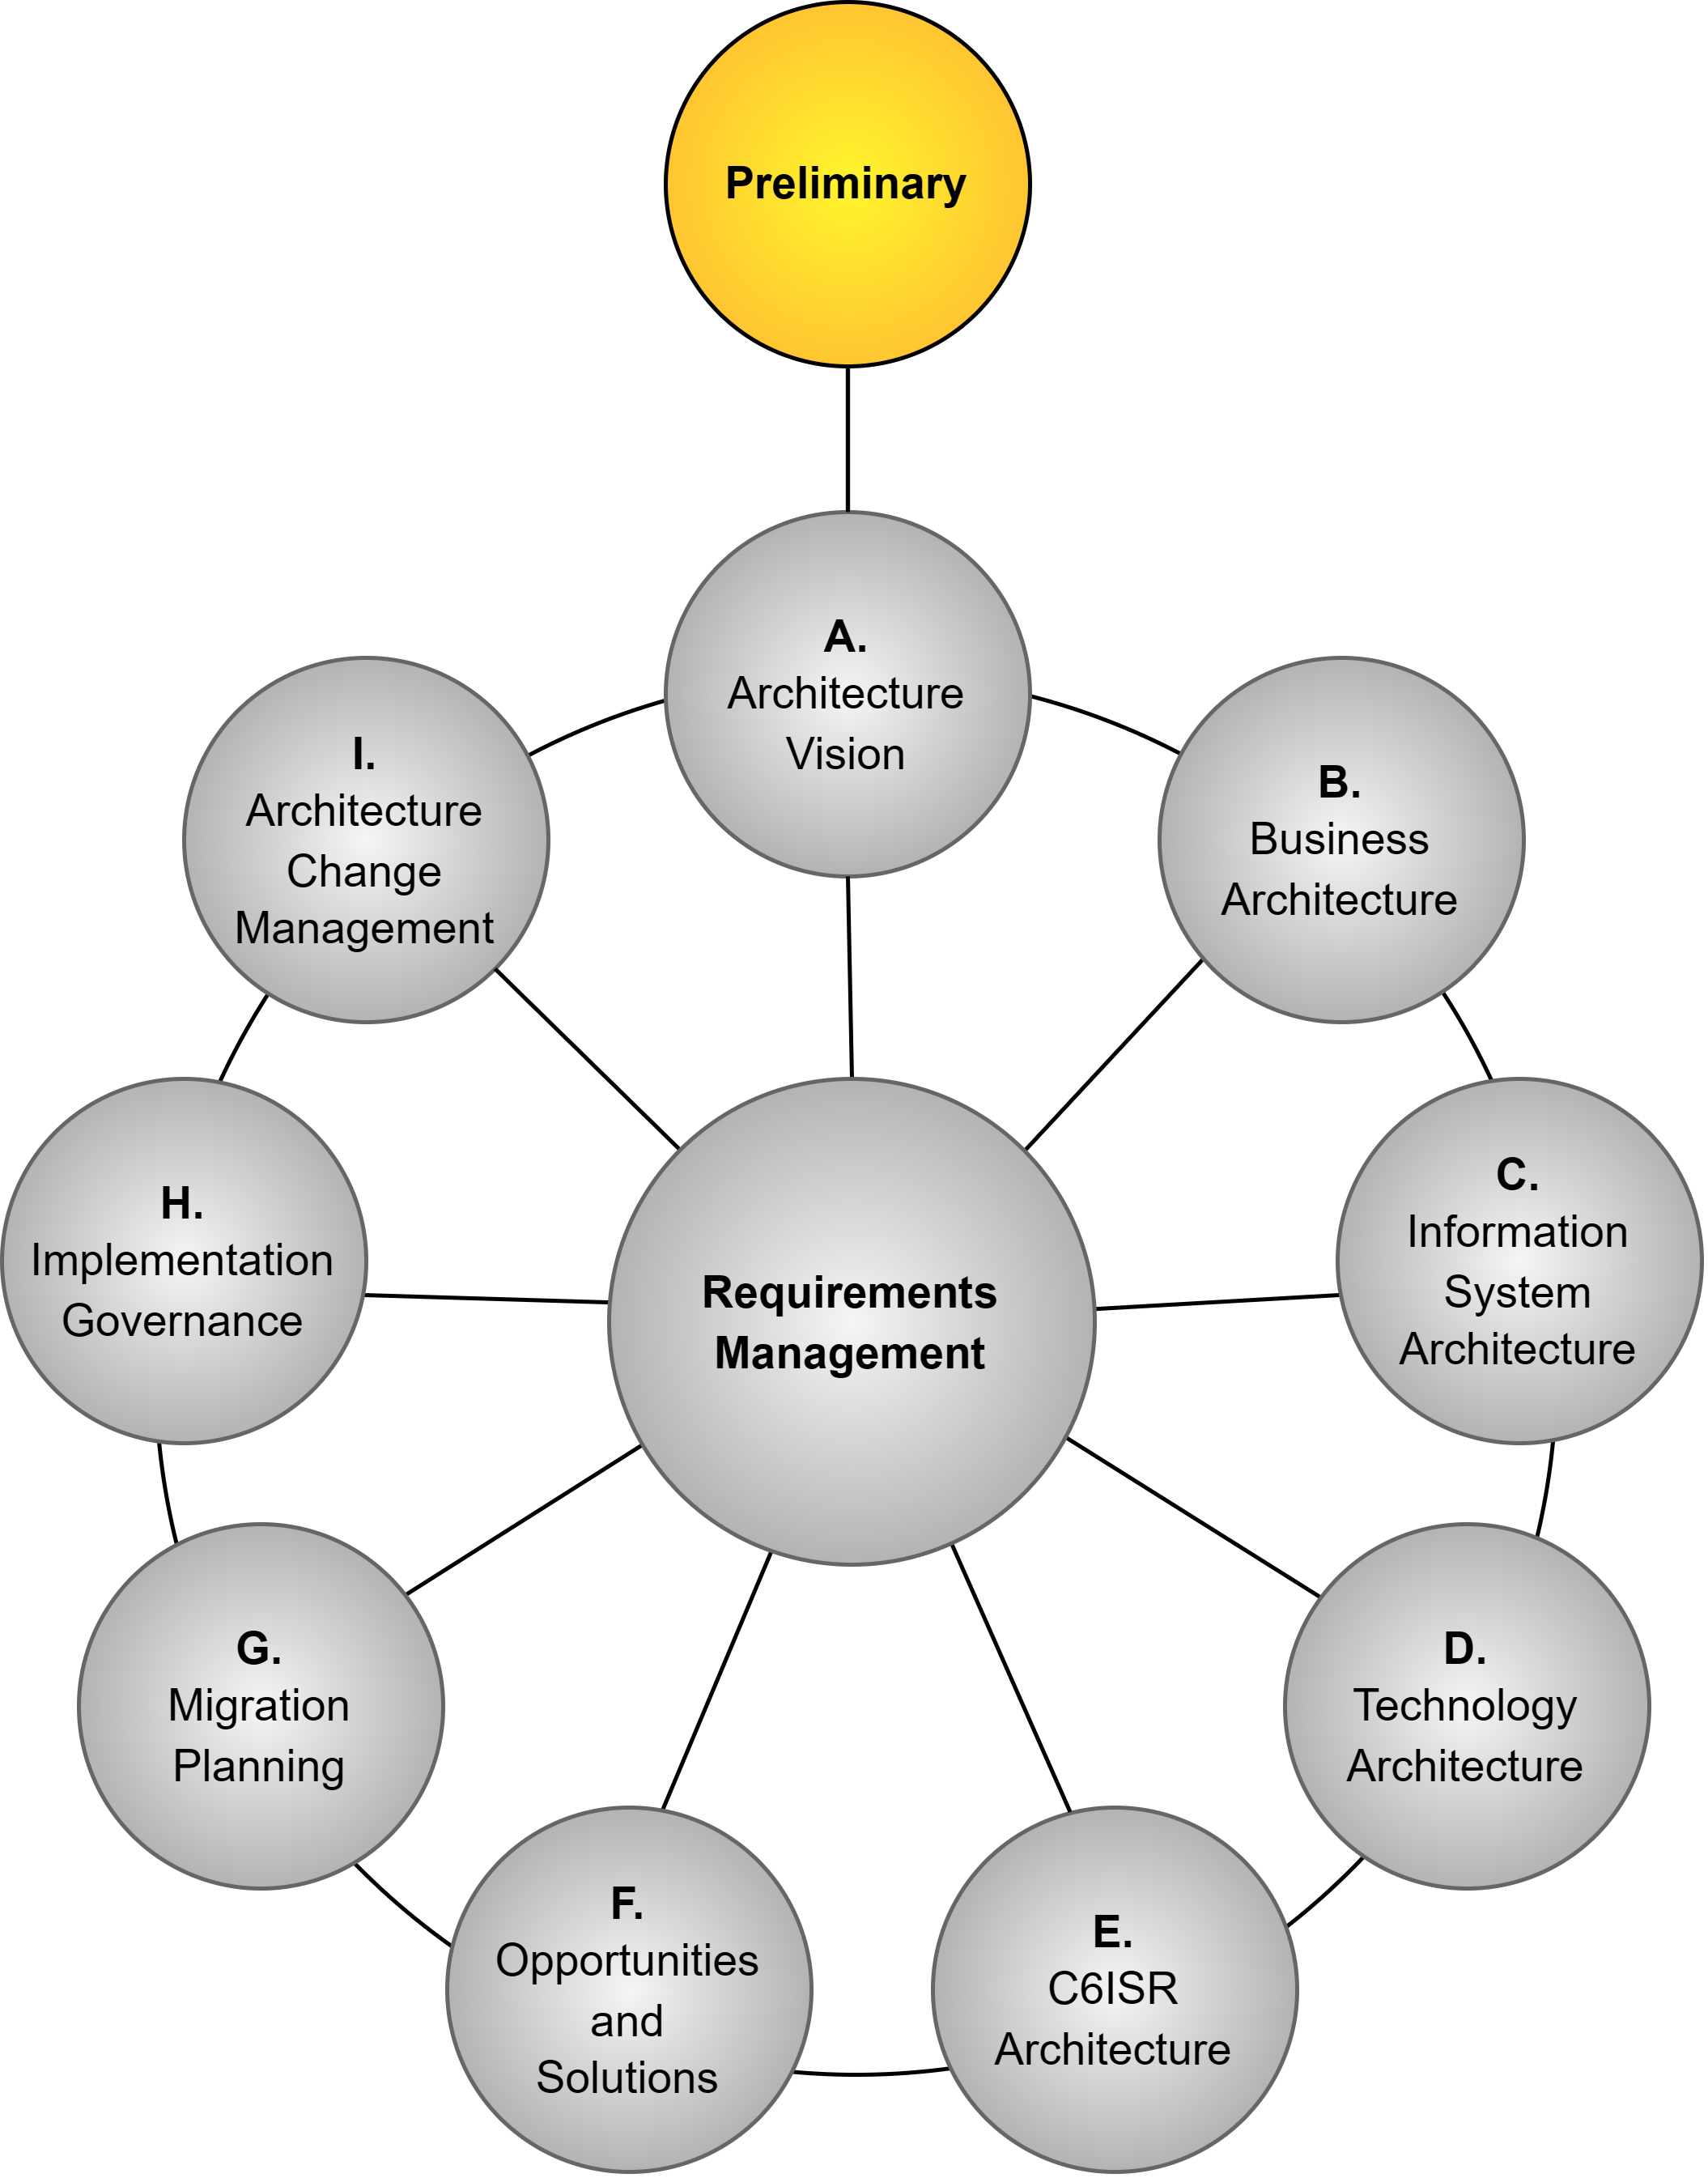
\includegraphics[width=0.46\linewidth,height=0.8\textheight,keepaspectratio]{images/Fase Preliminary.drawio.png}
\caption{Fase Preliminary}
\label{fig:III.3}
\end{figure}

Input, step, dan output Fase \textit{Preliminary} disajikan pada Tabel~\ref{tab:III.7}.

\begingroup\small\setstretch{1.0}
\begin{longtable}{@{}>{\raggedright\arraybackslash\hspace{0pt}}p{0.312\linewidth}>{\raggedright\arraybackslash\hspace{0pt}}p{0.312\linewidth}>{\raggedright\arraybackslash\hspace{0pt}}p{0.312\linewidth}@{}}
\caption{Input, Step, dan Output Fase \textit{Preliminary}}\label{tab:III.7}\\
\toprule
\textbf{INPUT} & \textbf{STEP} & \textbf{OUTPUT}\\
\midrule
\endfirsthead
\multicolumn{3}{@{}l}{\small\itshape \tablename\ \thetable{} (lanjutan)}\\
\toprule
\textbf{INPUT} & \textbf{STEP} & \textbf{OUTPUT}\\
\midrule
\endhead
\bottomrule
\endlastfoot
\hangindent=1.1em\hangafter=1 \makebox[1.1em][l]{1.}\textit{TOGAF reference material}\par \hangindent=1.1em\hangafter=1 \makebox[1.1em][l]{2.}Kerangka arsitektur pertahanan (DoDAF, NAF, dan MODAF) sebagai rujukan (+)\par \hangindent=1.1em\hangafter=1 \makebox[1.1em][l]{3.}Doktrin dan strategi pertahanan nasional (+)\par \hangindent=1.1em\hangafter=1 \makebox[1.1em][l]{4.}Regulasi SPBE, Arsitektur SPBE, dan Satu Data Pertahanan (+)\par \hangindent=1.1em\hangafter=1 \makebox[1.1em][l]{5.}Struktur organisasi dan pemangku kepentingan Kemhan RI\par \hangindent=1.1em\hangafter=1 \makebox[1.1em][l]{6.}Kapabilitas arsitektur yang dimiliki organisasi & \hangindent=1.1em\hangafter=1 \makebox[1.1em][l]{1.}Menetapkan ruang lingkup organisasi yang terdampak\par \hangindent=1.1em\hangafter=1 \makebox[1.1em][l]{2.}Mengonfirmasi kerangka tata kelola dan kerangka pendukung\par \hangindent=1.1em\hangafter=1 \makebox[1.1em][l]{3.}Membentuk tim \textit{Enterprise Architecture}\par \hangindent=1.1em\hangafter=1 \makebox[1.1em][l]{4.}Menetapkan prinsip arsitektur Pertahanan Indonesia (Δ)\par \hangindent=1.1em\hangafter=1 \makebox[1.1em][l]{5.}Menyesuaikan TOGAF ADM menjadi TOGAF Pertahanan Indonesia\par \hangindent=1.1em\hangafter=1 \makebox[1.1em][l]{6.}Memetakan keterkaitan arsitektur dengan regulasi nasional dan sektor pertahanan (+) & \hangindent=1.1em\hangafter=1 \makebox[1.1em][l]{1.}Model organisasi untuk arsitektur enterprise\par \hangindent=1.1em\hangafter=1 \makebox[1.1em][l]{2.}TOGAF Pertahanan Indonesia\par \hangindent=1.1em\hangafter=1 \makebox[1.1em][l]{3.}Prinsip arsitektur Pertahanan Indonesia (Δ)\par \hangindent=1.1em\hangafter=1 \makebox[1.1em][l]{4.}Kerangka tata kelola arsitektur\par \hangindent=1.1em\hangafter=1 \makebox[1.1em][l]{5.}\textit{Architecture Repository} awal\par \hangindent=1.1em\hangafter=1 \makebox[1.1em][l]{6.}Dokumen keterkaitan regulasi (+)\par \hangindent=1.1em\hangafter=1 \makebox[1.1em][l]{7.}\textit{Request for Architecture Work}\\
\end{longtable}
\endgroup

Keterangan: (+) = muatan baru; (Δ) = muatan TOGAF yang disesuaikan; tanpa tanda = TOGAF ADM standar.

Tabel~\ref{tab:III.7} menunjukkan bahwa muatan pertahanan ditanamkan sejak fase paling awal melalui doktrin, strategi pertahanan, dan regulasi nasional sebagai input. Muatan tersebut diwujudkan dalam sembilan prinsip arsitektur (Tabel~\ref{tab:III.6}) yang mengikat seluruh fase berikutnya.

\subsection{Fase \textit{Architecture Vision}}
\label{sec:III.3.2}

Fase Architecture Vision merumuskan visi, tujuan, dan ruang lingkup arsitektur, kemudian memperoleh persetujuan melalui \textit{Statement of Architecture Work}. Pada TOGAF Pertahanan Indonesia, visi tersebut diarahkan pada pertahanan cerdas. Kedudukan fase ini ditunjukkan pada Gambar~\ref{fig:III.4}.
\begin{figure}[htbp]
\centering
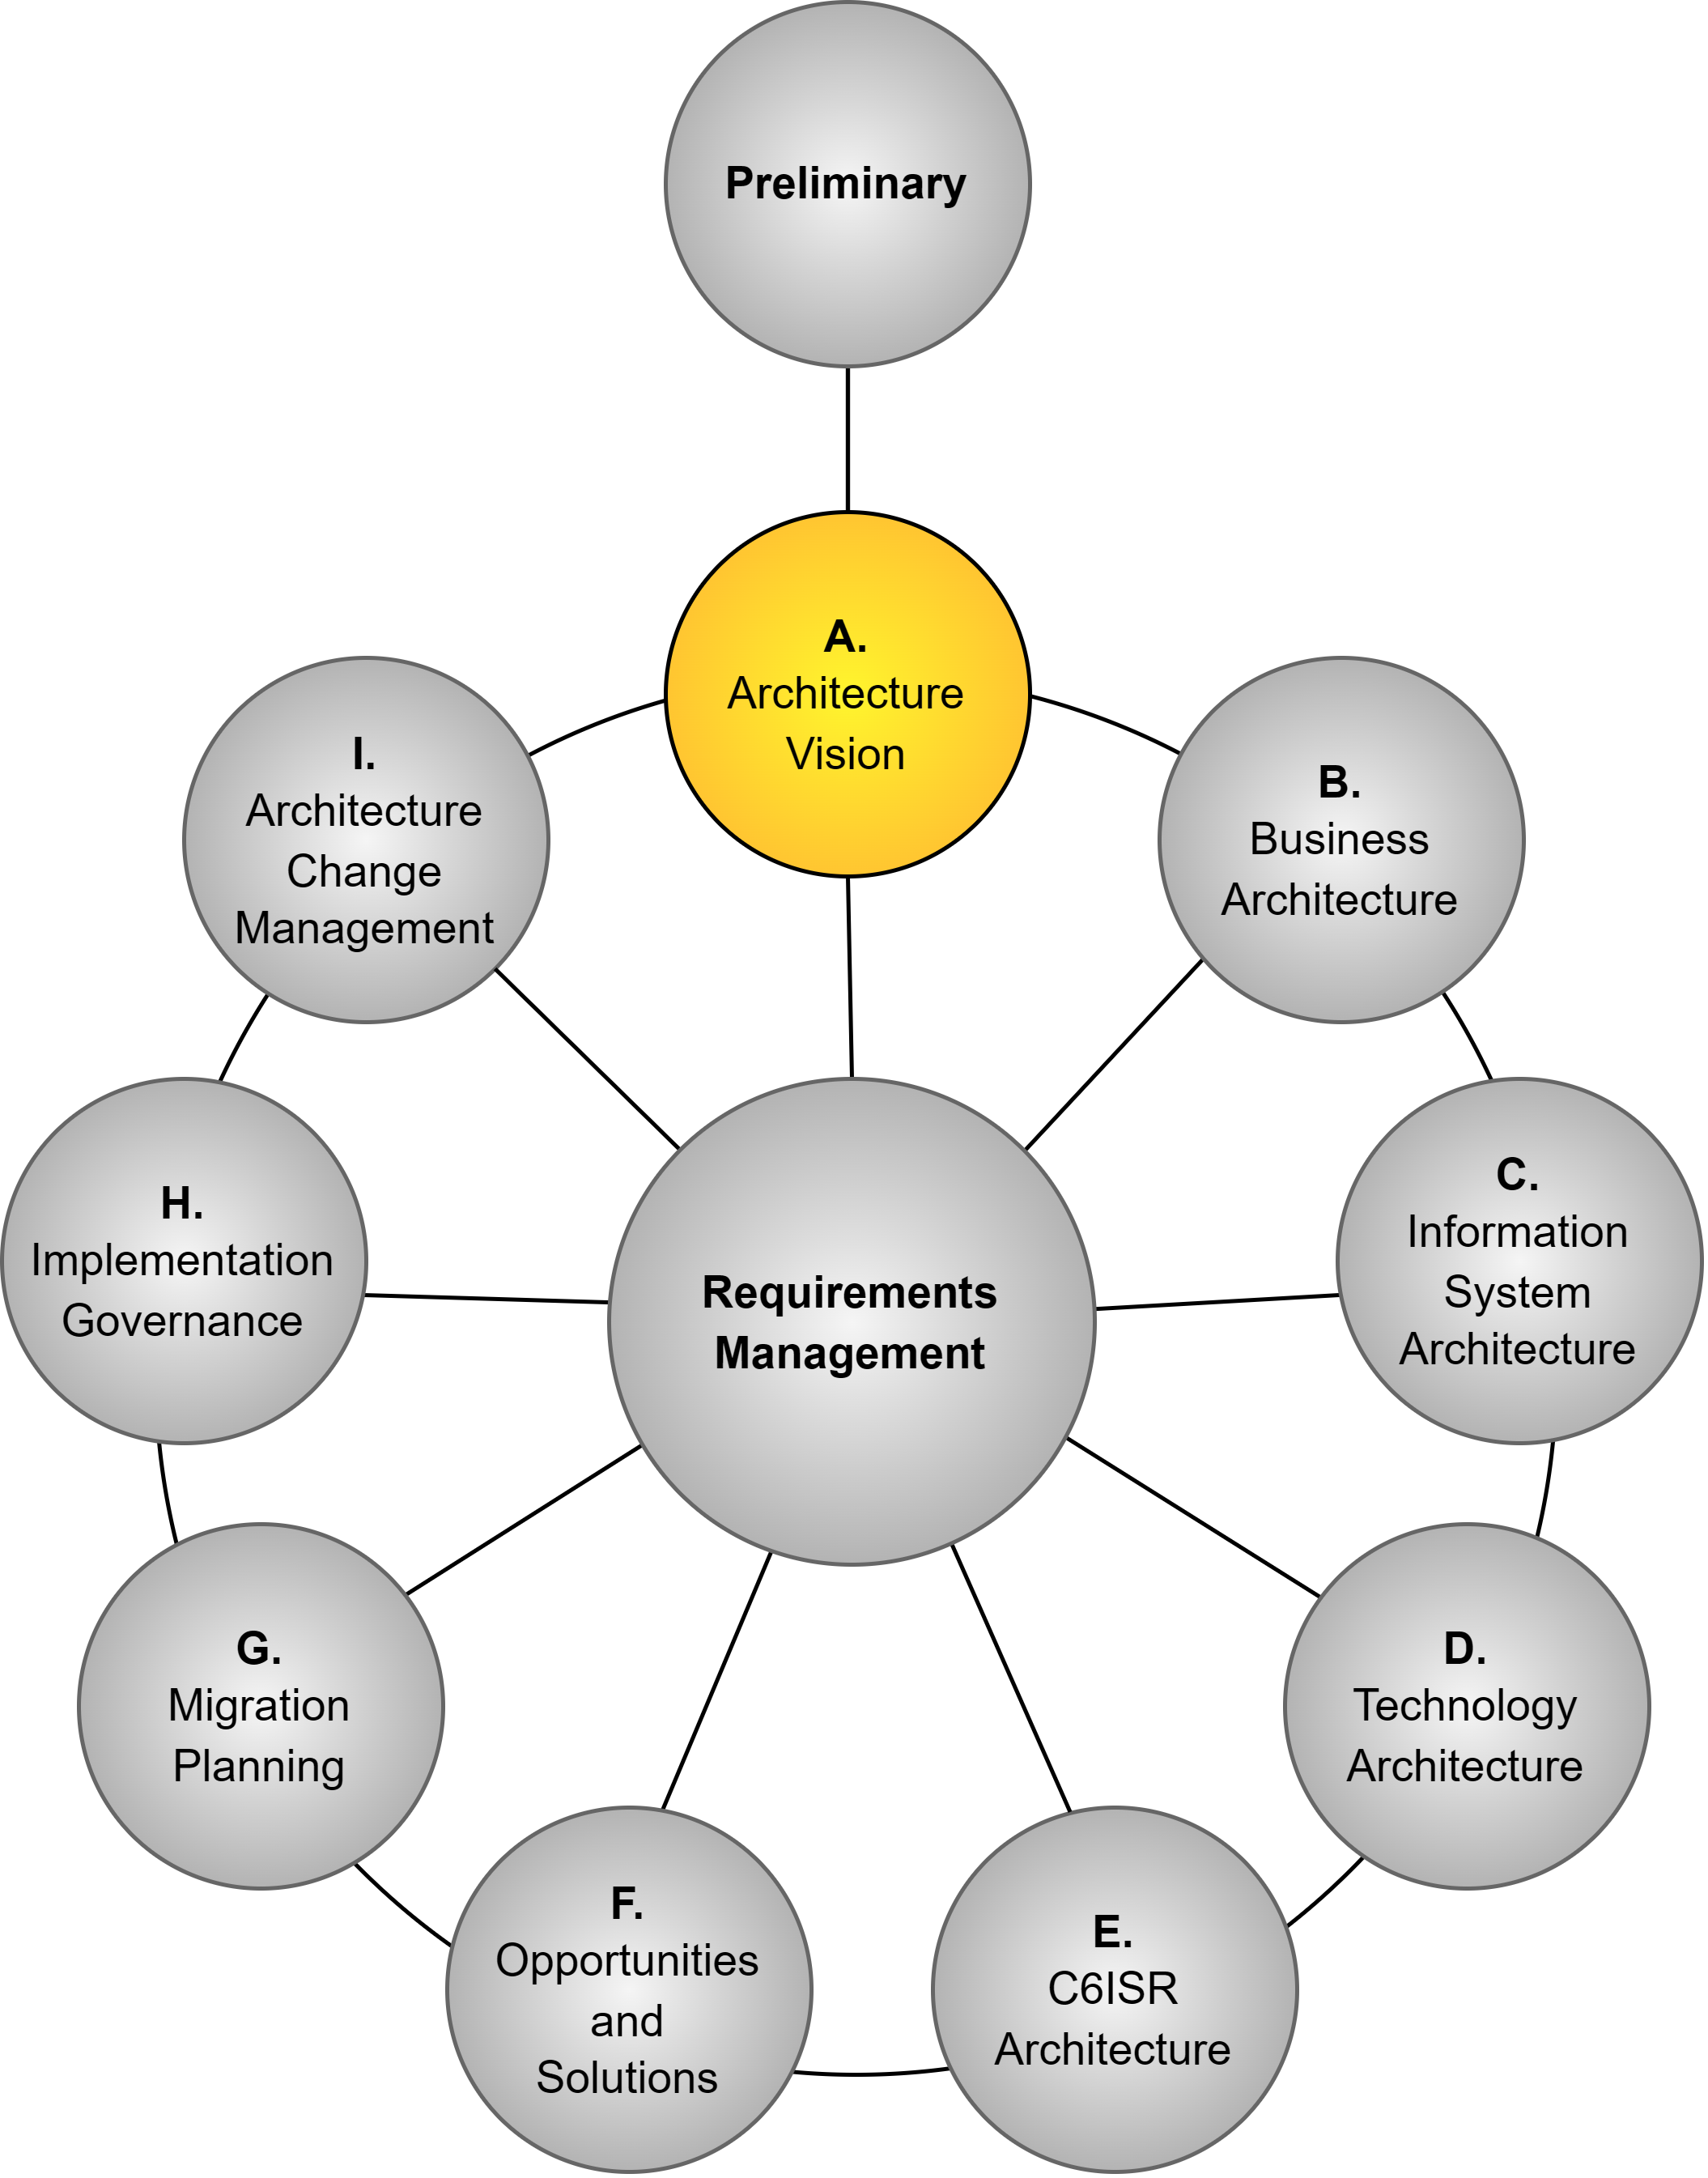
\includegraphics[width=0.46\linewidth,height=0.8\textheight,keepaspectratio]{images/Fase Architecture Vision.drawio.png}
\caption{Fase \textit{Architecture Vision}}
\label{fig:III.4}
\end{figure}

Input, step, dan output Fase \textit{Architecture Vision} disajikan pada Tabel~\ref{tab:III.8}.

\begingroup\small\setstretch{1.0}
\begin{longtable}{@{}>{\raggedright\arraybackslash\hspace{0pt}}p{0.312\linewidth}>{\raggedright\arraybackslash\hspace{0pt}}p{0.312\linewidth}>{\raggedright\arraybackslash\hspace{0pt}}p{0.312\linewidth}@{}}
\caption{Input, Step, dan Output Fase \textit{Architecture Vision}}\label{tab:III.8}\\
\toprule
\textbf{INPUT} & \textbf{STEP} & \textbf{OUTPUT}\\
\midrule
\endfirsthead
\multicolumn{3}{@{}l}{\small\itshape \tablename\ \thetable{} (lanjutan)}\\
\toprule
\textbf{INPUT} & \textbf{STEP} & \textbf{OUTPUT}\\
\midrule
\endhead
\bottomrule
\endlastfoot
\hangindent=1.1em\hangafter=1 \makebox[1.1em][l]{1.}\textit{Request for Architecture Work}\par \hangindent=1.1em\hangafter=1 \makebox[1.1em][l]{2.}Prinsip arsitektur Pertahanan Indonesia\par \hangindent=1.1em\hangafter=1 \makebox[1.1em][l]{3.}Model organisasi dan TOGAF Pertahanan Indonesia\par \hangindent=1.1em\hangafter=1 \makebox[1.1em][l]{4.}\textit{Architecture Repository}\par \hangindent=1.1em\hangafter=1 \makebox[1.1em][l]{5.}Doktrin, strategi pertahanan, dan regulasi nasional (+) & \hangindent=1.1em\hangafter=1 \makebox[1.1em][l]{1.}Menetapkan proyek arsitektur\par \hangindent=1.1em\hangafter=1 \makebox[1.1em][l]{2.}Mengidentifikasi pemangku kepentingan dan \textit{concern}\par \hangindent=1.1em\hangafter=1 \makebox[1.1em][l]{3.}Mengonfirmasi sasaran, pendorong, dan kendala transformasi pertahanan (Δ)\par \hangindent=1.1em\hangafter=1 \makebox[1.1em][l]{4.}Menilai kapabilitas dan kesiapan transformasi\par \hangindent=1.1em\hangafter=1 \makebox[1.1em][l]{5.}Menyusun visi dan misi arsitektur yang berorientasi pada pertahanan cerdas (Δ)\par \hangindent=1.1em\hangafter=1 \makebox[1.1em][l]{6.}Menetapkan nilai manfaat dan indikator kinerja\par \hangindent=1.1em\hangafter=1 \makebox[1.1em][l]{7.}Mengidentifikasi risiko transformasi dan mitigasinya\par \hangindent=1.1em\hangafter=1 \makebox[1.1em][l]{8.}Menyusun \textit{Statement of Architecture Work} dan memperoleh persetujuan & \hangindent=1.1em\hangafter=1 \makebox[1.1em][l]{1.}\textit{Statement of Architecture Work} yang disetujui\par \hangindent=1.1em\hangafter=1 \makebox[1.1em][l]{2.}Dokumen \textit{Architecture Vision} (Δ)\par \hangindent=1.1em\hangafter=1 \makebox[1.1em][l]{3.}Peta pemangku kepentingan\par \hangindent=1.1em\hangafter=1 \makebox[1.1em][l]{4.}Hasil penilaian kapabilitas dan kesiapan\par \hangindent=1.1em\hangafter=1 \makebox[1.1em][l]{5.}Tujuan strategis arsitektur (Δ)\par \hangindent=1.1em\hangafter=1 \makebox[1.1em][l]{6.}Rencana komunikasi\\
\end{longtable}
\endgroup

Keterangan: (+) = muatan baru; (Δ) = muatan TOGAF yang disesuaikan; tanpa tanda = TOGAF ADM standar.

Tabel~\ref{tab:III.8} menunjukkan bahwa visi arsitektur diturunkan dari doktrin, strategi pertahanan, dan regulasi nasional. Dengan demikian, arah transformasi digital tetap selaras dengan kebijakan pertahanan, sedangkan pemangku kepentingan yang berjenjang di lingkungan Kemhan RI dan TNI diakomodasi melalui peta pemangku kepentingan.

\subsection{Fase \textit{Business Architecture}}
\label{sec:III.3.3}

Fase Business Architecture merancang kapabilitas, proses bisnis, dan organisasi yang mendukung komando-kendali serta kolaborasi lintas satuan. Fase ini menjadi pijakan bagi perancangan data, aplikasi, teknologi, dan C6ISR. Kedudukan fase ini ditunjukkan pada Gambar~\ref{fig:III.5}.
\begin{figure}[htbp]
\centering
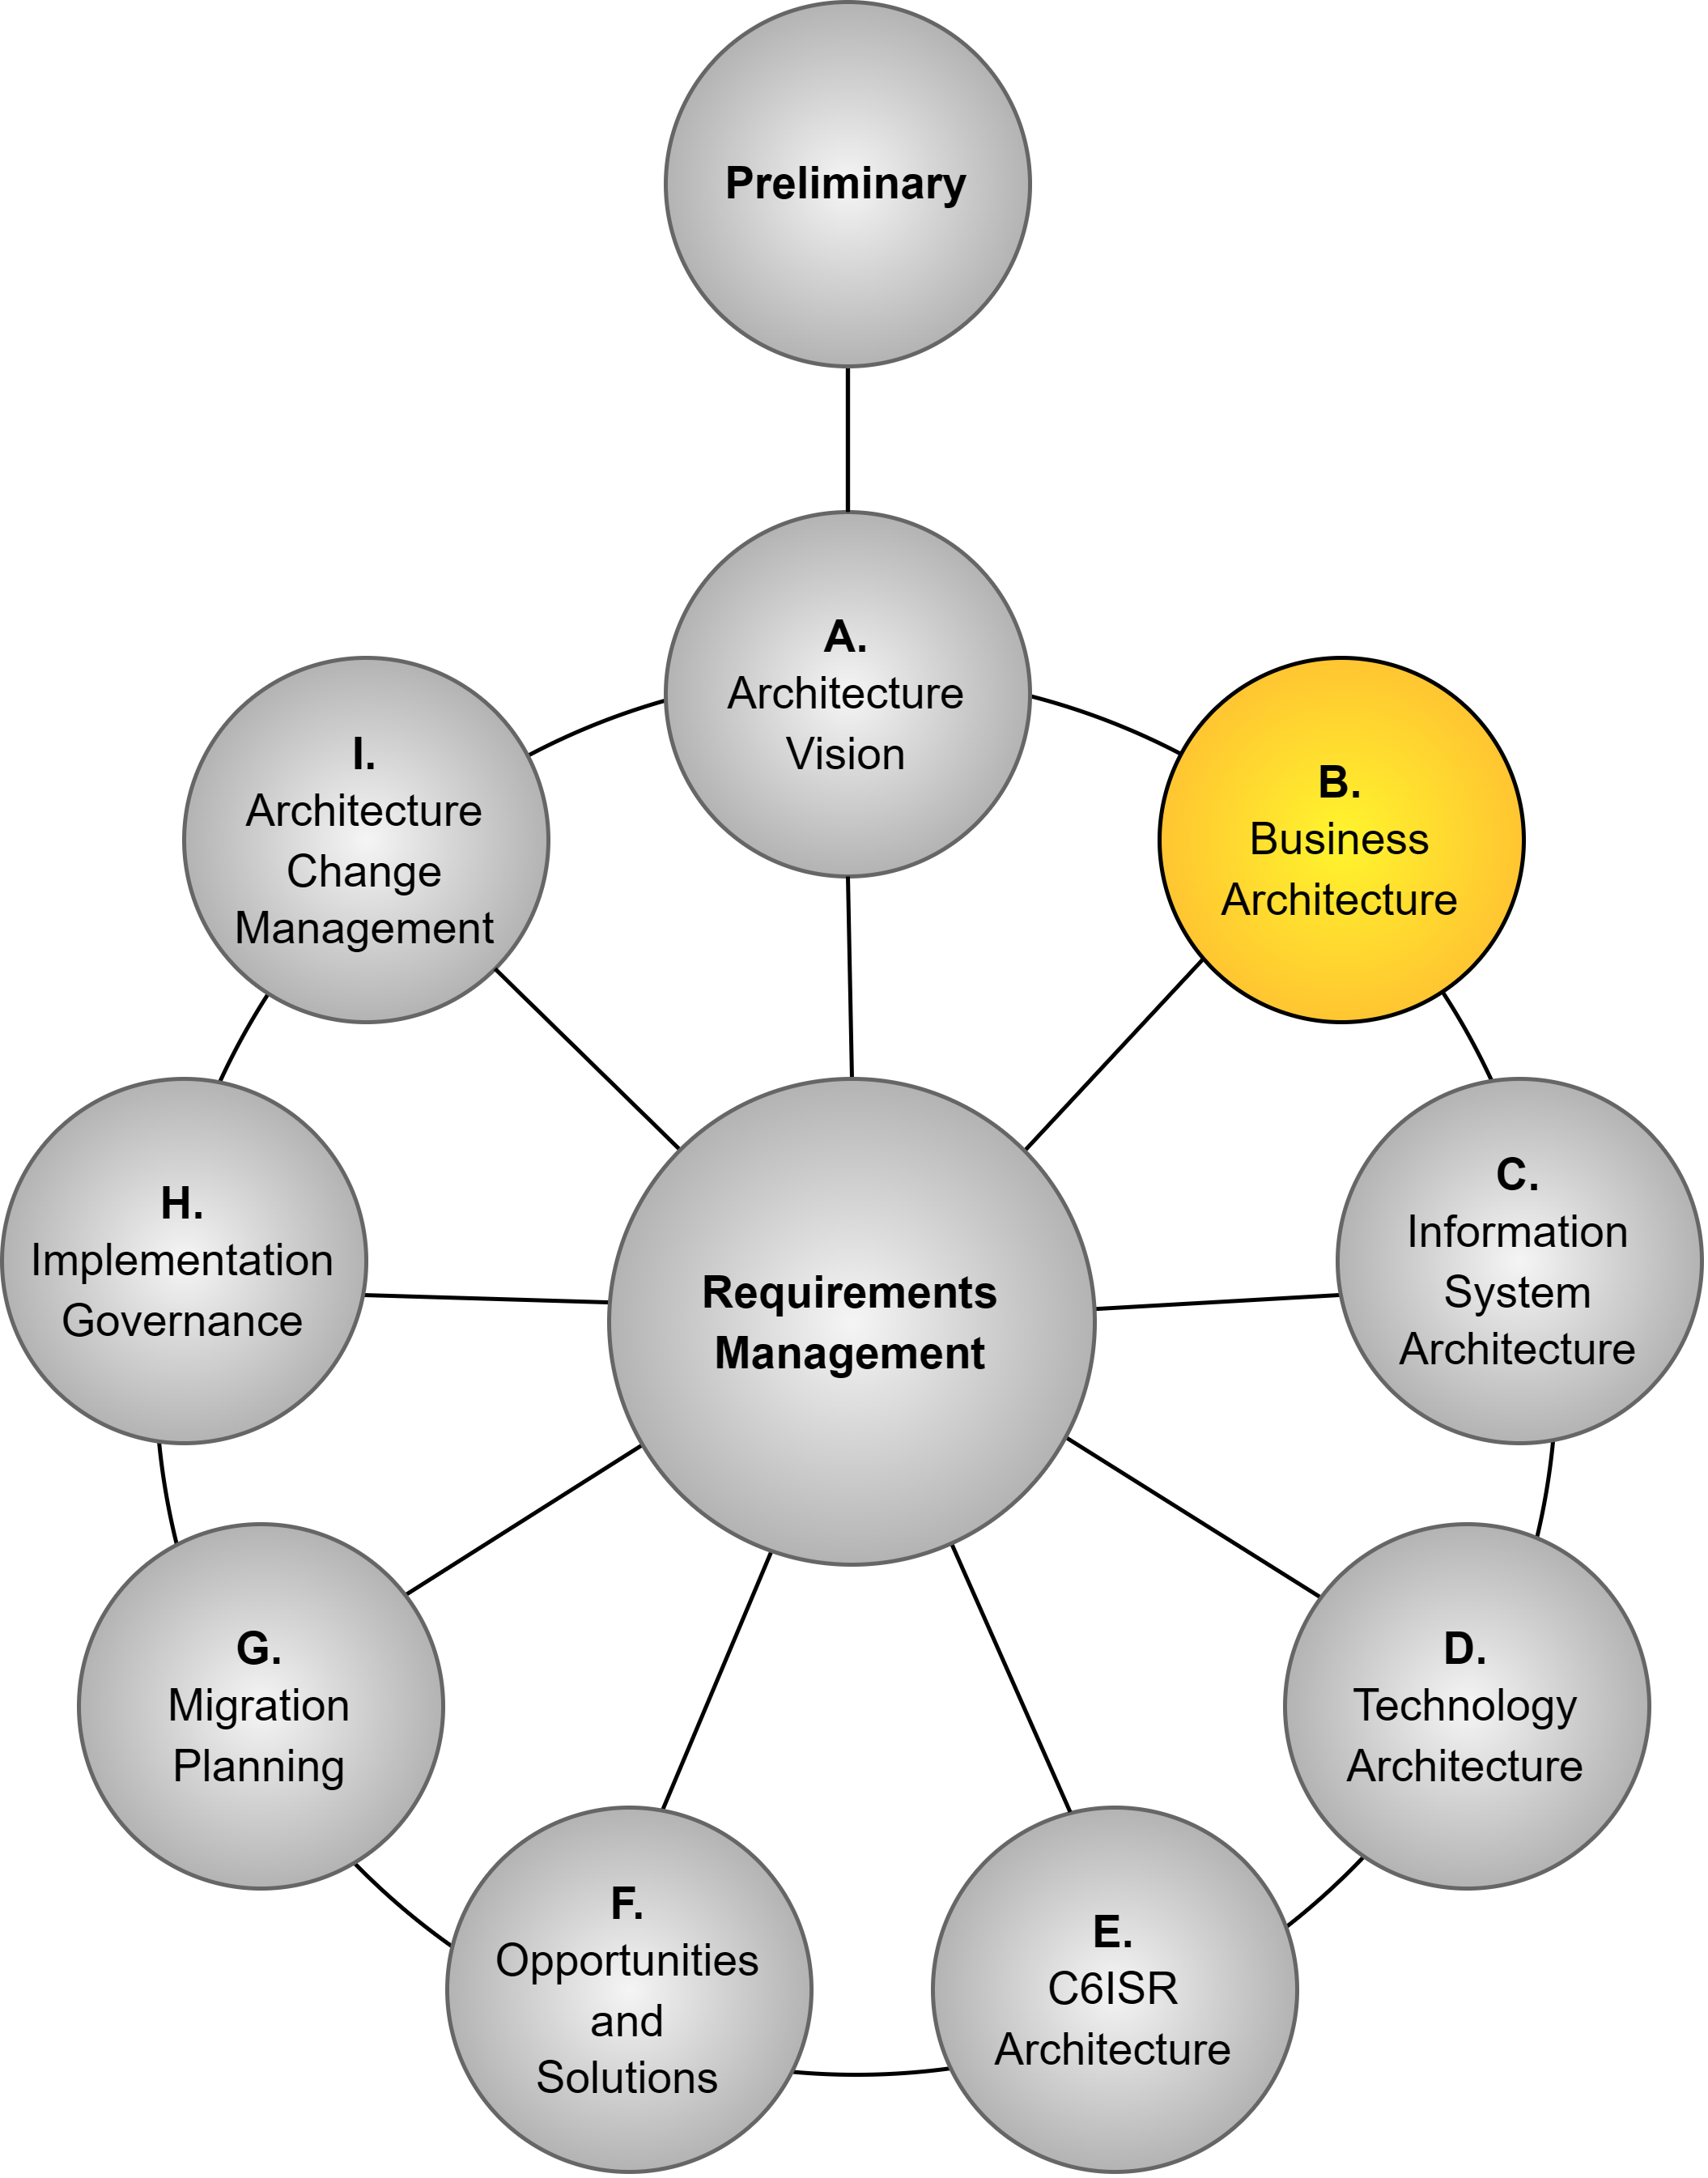
\includegraphics[width=0.46\linewidth,height=0.8\textheight,keepaspectratio]{images/Fase Business Architecture.drawio.png}
\caption{Fase \textit{Business Architecture}}
\label{fig:III.5}
\end{figure}

Input, step, dan output Fase \textit{Business Architecture} disajikan pada Tabel~\ref{tab:III.9}.

\begingroup\small\setstretch{1.0}
\begin{longtable}{@{}>{\raggedright\arraybackslash\hspace{0pt}}p{0.312\linewidth}>{\raggedright\arraybackslash\hspace{0pt}}p{0.312\linewidth}>{\raggedright\arraybackslash\hspace{0pt}}p{0.312\linewidth}@{}}
\caption{Input, Step, dan Output Fase \textit{Business Architecture}}\label{tab:III.9}\\
\toprule
\textbf{INPUT} & \textbf{STEP} & \textbf{OUTPUT}\\
\midrule
\endfirsthead
\multicolumn{3}{@{}l}{\small\itshape \tablename\ \thetable{} (lanjutan)}\\
\toprule
\textbf{INPUT} & \textbf{STEP} & \textbf{OUTPUT}\\
\midrule
\endhead
\bottomrule
\endlastfoot
\hangindent=1.1em\hangafter=1 \makebox[1.1em][l]{1.}\textit{Statement of Architecture Work} dan dokumen \textit{Architecture Vision}\par \hangindent=1.1em\hangafter=1 \makebox[1.1em][l]{2.}Prinsip arsitektur Pertahanan Indonesia\par \hangindent=1.1em\hangafter=1 \makebox[1.1em][l]{3.}\textit{Architecture Repository}\par \hangindent=1.1em\hangafter=1 \makebox[1.1em][l]{4.}Struktur organisasi dan proses bisnis Kemhan RI saat ini\par \hangindent=1.1em\hangafter=1 \makebox[1.1em][l]{5.}Strategi pertahanan dan transformasi digital (+) & \hangindent=1.1em\hangafter=1 \makebox[1.1em][l]{1.}Memilih model rujukan, \textit{viewpoint}, dan perangkat pemodelan\par \hangindent=1.1em\hangafter=1 \makebox[1.1em][l]{2.}Menyusun arsitektur \textit{bisnis baseline}\par \hangindent=1.1em\hangafter=1 \makebox[1.1em][l]{3.}Menyusun \textit{value stream} dan peta kapabilitas pertahanan (Δ)\par \hangindent=1.1em\hangafter=1 \makebox[1.1em][l]{4.}Menyusun arsitektur bisnis target\par \hangindent=1.1em\hangafter=1 \makebox[1.1em][l]{5.}Melakukan analisis kesenjangan\par \hangindent=1.1em\hangafter=1 \makebox[1.1em][l]{6.}Menetapkan komponen \textit{roadmap}\par \hangindent=1.1em\hangafter=1 \makebox[1.1em][l]{7.}Melaksanakan tinjauan pemangku kepentingan dan memfinalkan arsitektur bisnis & \hangindent=1.1em\hangafter=1 \makebox[1.1em][l]{1.}\textit{Draf Architecture Definition Document} dan \textit{Architecture Requirements Specification}\par \hangindent=1.1em\hangafter=1 \makebox[1.1em][l]{2.}\textit{Value stream} dan peta kapabilitas pertahanan (Δ)\par \hangindent=1.1em\hangafter=1 \makebox[1.1em][l]{3.}Model tata kelola dan komando (+)\par \hangindent=1.1em\hangafter=1 \makebox[1.1em][l]{4.}Model operasi dan interoperabilitas lintas matra (+)\par \hangindent=1.1em\hangafter=1 \makebox[1.1em][l]{5.}Komponen arsitektur bisnis pada \textit{roadmap}\\
\end{longtable}
\endgroup

Keterangan: (+) = muatan baru; (Δ) = muatan TOGAF yang disesuaikan; tanpa tanda = TOGAF ADM standar.

Tabel~\ref{tab:III.9} menunjukkan bahwa fase ini menggunakan pendekatan berbasis kapabilitas. Model tata kelola dan komando serta model interoperabilitas lintas matra menjadi output dari fase ini.

\subsection{Fase \textit{Information Systems Architecture}}
\label{sec:III.3.4}

Fase \textit{Information Systems Architecture} merancang arsitektur data dan arsitektur aplikasi yang mendukung proses bisnis pertahanan. Pada TOGAF Pertahanan Indonesia, arsitektur data dikerjakan lebih dahulu karena permasalahan utama terletak pada data yang terkotak-kotak antarsatuan. Oleh karena itu, definisi, klasifikasi, dan kepemilikan data ditetapkan sebelum portofolio aplikasi dirancang. Kedua subdomain tersebut diuraikan sebagai berikut.

\subsubsection{\textit{Data Architecture}}
\label{sec:III.3.4.1}

Data Architecture merancang definisi, klasifikasi, dan kepemilikan data pertahanan. Perancangannya berpedoman pada prinsip \textit{Data as Strategic Asset} serta ketentuan Satu Data dan klasifikasi informasi pertahanan. Kedudukan subdomain ini ditunjukkan pada Gambar~\ref{fig:III.6}.
\begin{figure}[htbp]
\centering
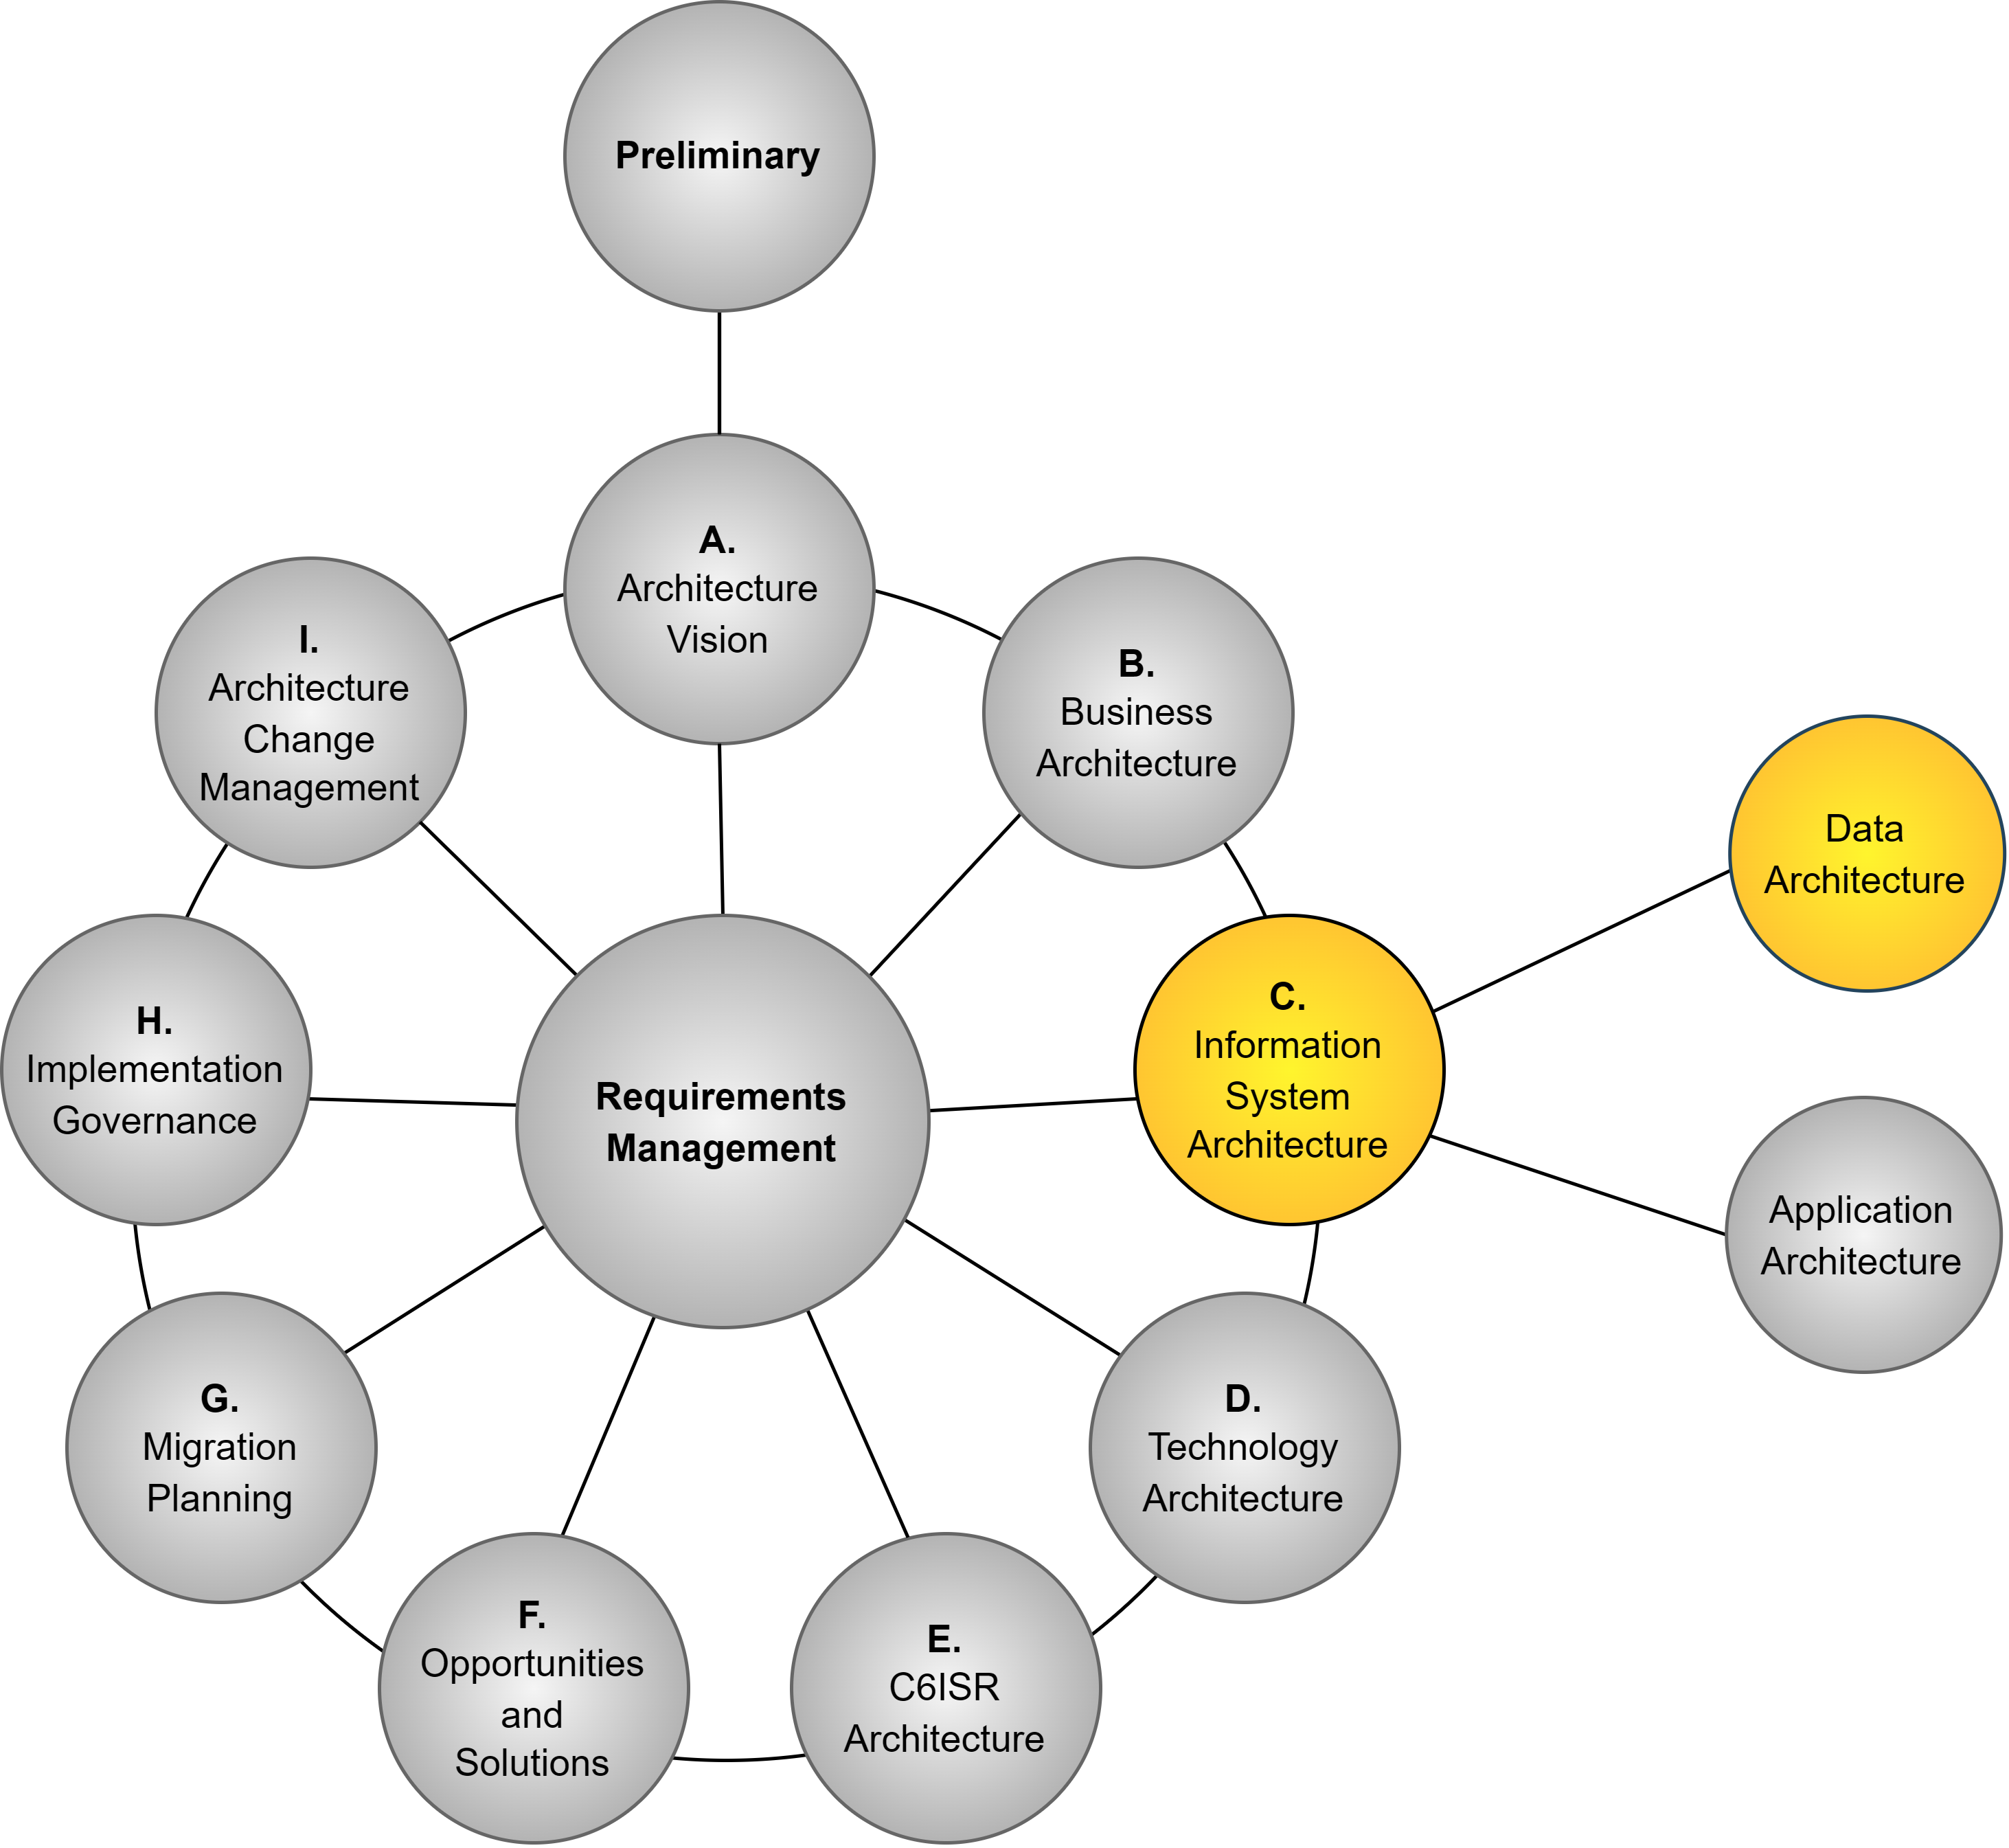
\includegraphics[width=0.61\linewidth,height=0.8\textheight,keepaspectratio]{images/Fase Data Architecture.drawio.png}
\caption{\textit{Data Architecture}}
\label{fig:III.6}
\end{figure}

Input, step, dan output \textit{Data Architecture} disajikan pada Tabel~\ref{tab:III.10}.

\begingroup\small\setstretch{1.0}
\begin{longtable}{@{}>{\raggedright\arraybackslash\hspace{0pt}}p{0.312\linewidth}>{\raggedright\arraybackslash\hspace{0pt}}p{0.312\linewidth}>{\raggedright\arraybackslash\hspace{0pt}}p{0.312\linewidth}@{}}
\caption{Input, Step, dan Output \textit{Data Architecture}}\label{tab:III.10}\\
\toprule
\textbf{INPUT} & \textbf{STEP} & \textbf{OUTPUT}\\
\midrule
\endfirsthead
\multicolumn{3}{@{}l}{\small\itshape \tablename\ \thetable{} (lanjutan)}\\
\toprule
\textbf{INPUT} & \textbf{STEP} & \textbf{OUTPUT}\\
\midrule
\endhead
\bottomrule
\endlastfoot
\hangindent=1.1em\hangafter=1 \makebox[1.1em][l]{1.}\textit{Statement of Architecture Work} dan dokumen \textit{Architecture Vision}\par \hangindent=1.1em\hangafter=1 \makebox[1.1em][l]{2.}Prinsip arsitektur Pertahanan Indonesia\par \hangindent=1.1em\hangafter=1 \makebox[1.1em][l]{3.}Komponen arsitektur bisnis pada roadmap\par \hangindent=1.1em\hangafter=1 \makebox[1.1em][l]{4.}Inventaris data Kemhan RI\par \hangindent=1.1em\hangafter=1 \makebox[1.1em][l]{5.}Regulasi Satu Data dan klasifikasi informasi pertahanan (+)\par \hangindent=1.1em\hangafter=1 \makebox[1.1em][l]{6.}Standar keamanan siber dan pelindungan data (+) & \hangindent=1.1em\hangafter=1 \makebox[1.1em][l]{1.}Memilih model rujukan, viewpoint, dan perangkat pemodelan data\par \hangindent=1.1em\hangafter=1 \makebox[1.1em][l]{2.}Menyusun arsitektur data baseline\par \hangindent=1.1em\hangafter=1 \makebox[1.1em][l]{3.}Memodelkan entitas data utama\par \hangindent=1.1em\hangafter=1 \makebox[1.1em][l]{4.}Menyusun klasifikasi kerahasiaan data (Δ)\par \hangindent=1.1em\hangafter=1 \makebox[1.1em][l]{5.}Menetapkan kepemilikan dan tata kelola data antarsatuan (Δ)\par \hangindent=1.1em\hangafter=1 \makebox[1.1em][l]{6.}Menyusun arsitektur data target\par \hangindent=1.1em\hangafter=1 \makebox[1.1em][l]{7.}Melakukan analisis kesenjangan dan menetapkan komponen \textit{roadmap} & \hangindent=1.1em\hangafter=1 \makebox[1.1em][l]{1.}Model entitas dan kamus data pertahanan\par \hangindent=1.1em\hangafter=1 \makebox[1.1em][l]{2.}Klasifikasi kerahasiaan data (Δ)\par \hangindent=1.1em\hangafter=1 \makebox[1.1em][l]{3.}Matriks kepemilikan dan tata kelola data (Δ)\par \hangindent=1.1em\hangafter=1 \makebox[1.1em][l]{4.}Rancangan keamanan dan kendali akses data (+)\par \hangindent=1.1em\hangafter=1 \makebox[1.1em][l]{5.}Komponen arsitektur data pada \textit{roadmap}\\
\end{longtable}
\endgroup

Keterangan: (+) = muatan baru; (Δ) = muatan TOGAF yang disesuaikan; tanpa tanda = TOGAF ADM standar.

Tabel~\ref{tab:III.10} menunjukkan bahwa klasifikasi kerahasiaan dan kendali akses menjadi batas sekaligus pengarah rancangan data, sehingga kewajiban berbagi pakai data tetap memperhatikan ketentuan kerahasiaan.

\subsubsection{\textit{Application Architecture}}
\label{sec:III.3.4.2}

\textit{Application Architecture} merancang portofolio aplikasi dan mekanisme keterhubungan antaraplikasi. Perancangannya berpedoman pada prinsip \textit{Interoperability} dan \textit{User-Centric Service}. Subdomain ini dikerjakan setelah \textit{Data Architecture} karena integrasi antaraplikasi hanya dapat dirancang di atas definisi data yang telah disepakati. Kedudukan subdomain ini ditunjukkan pada Gambar~\ref{fig:III.7}.
\begin{figure}[htbp]
\centering
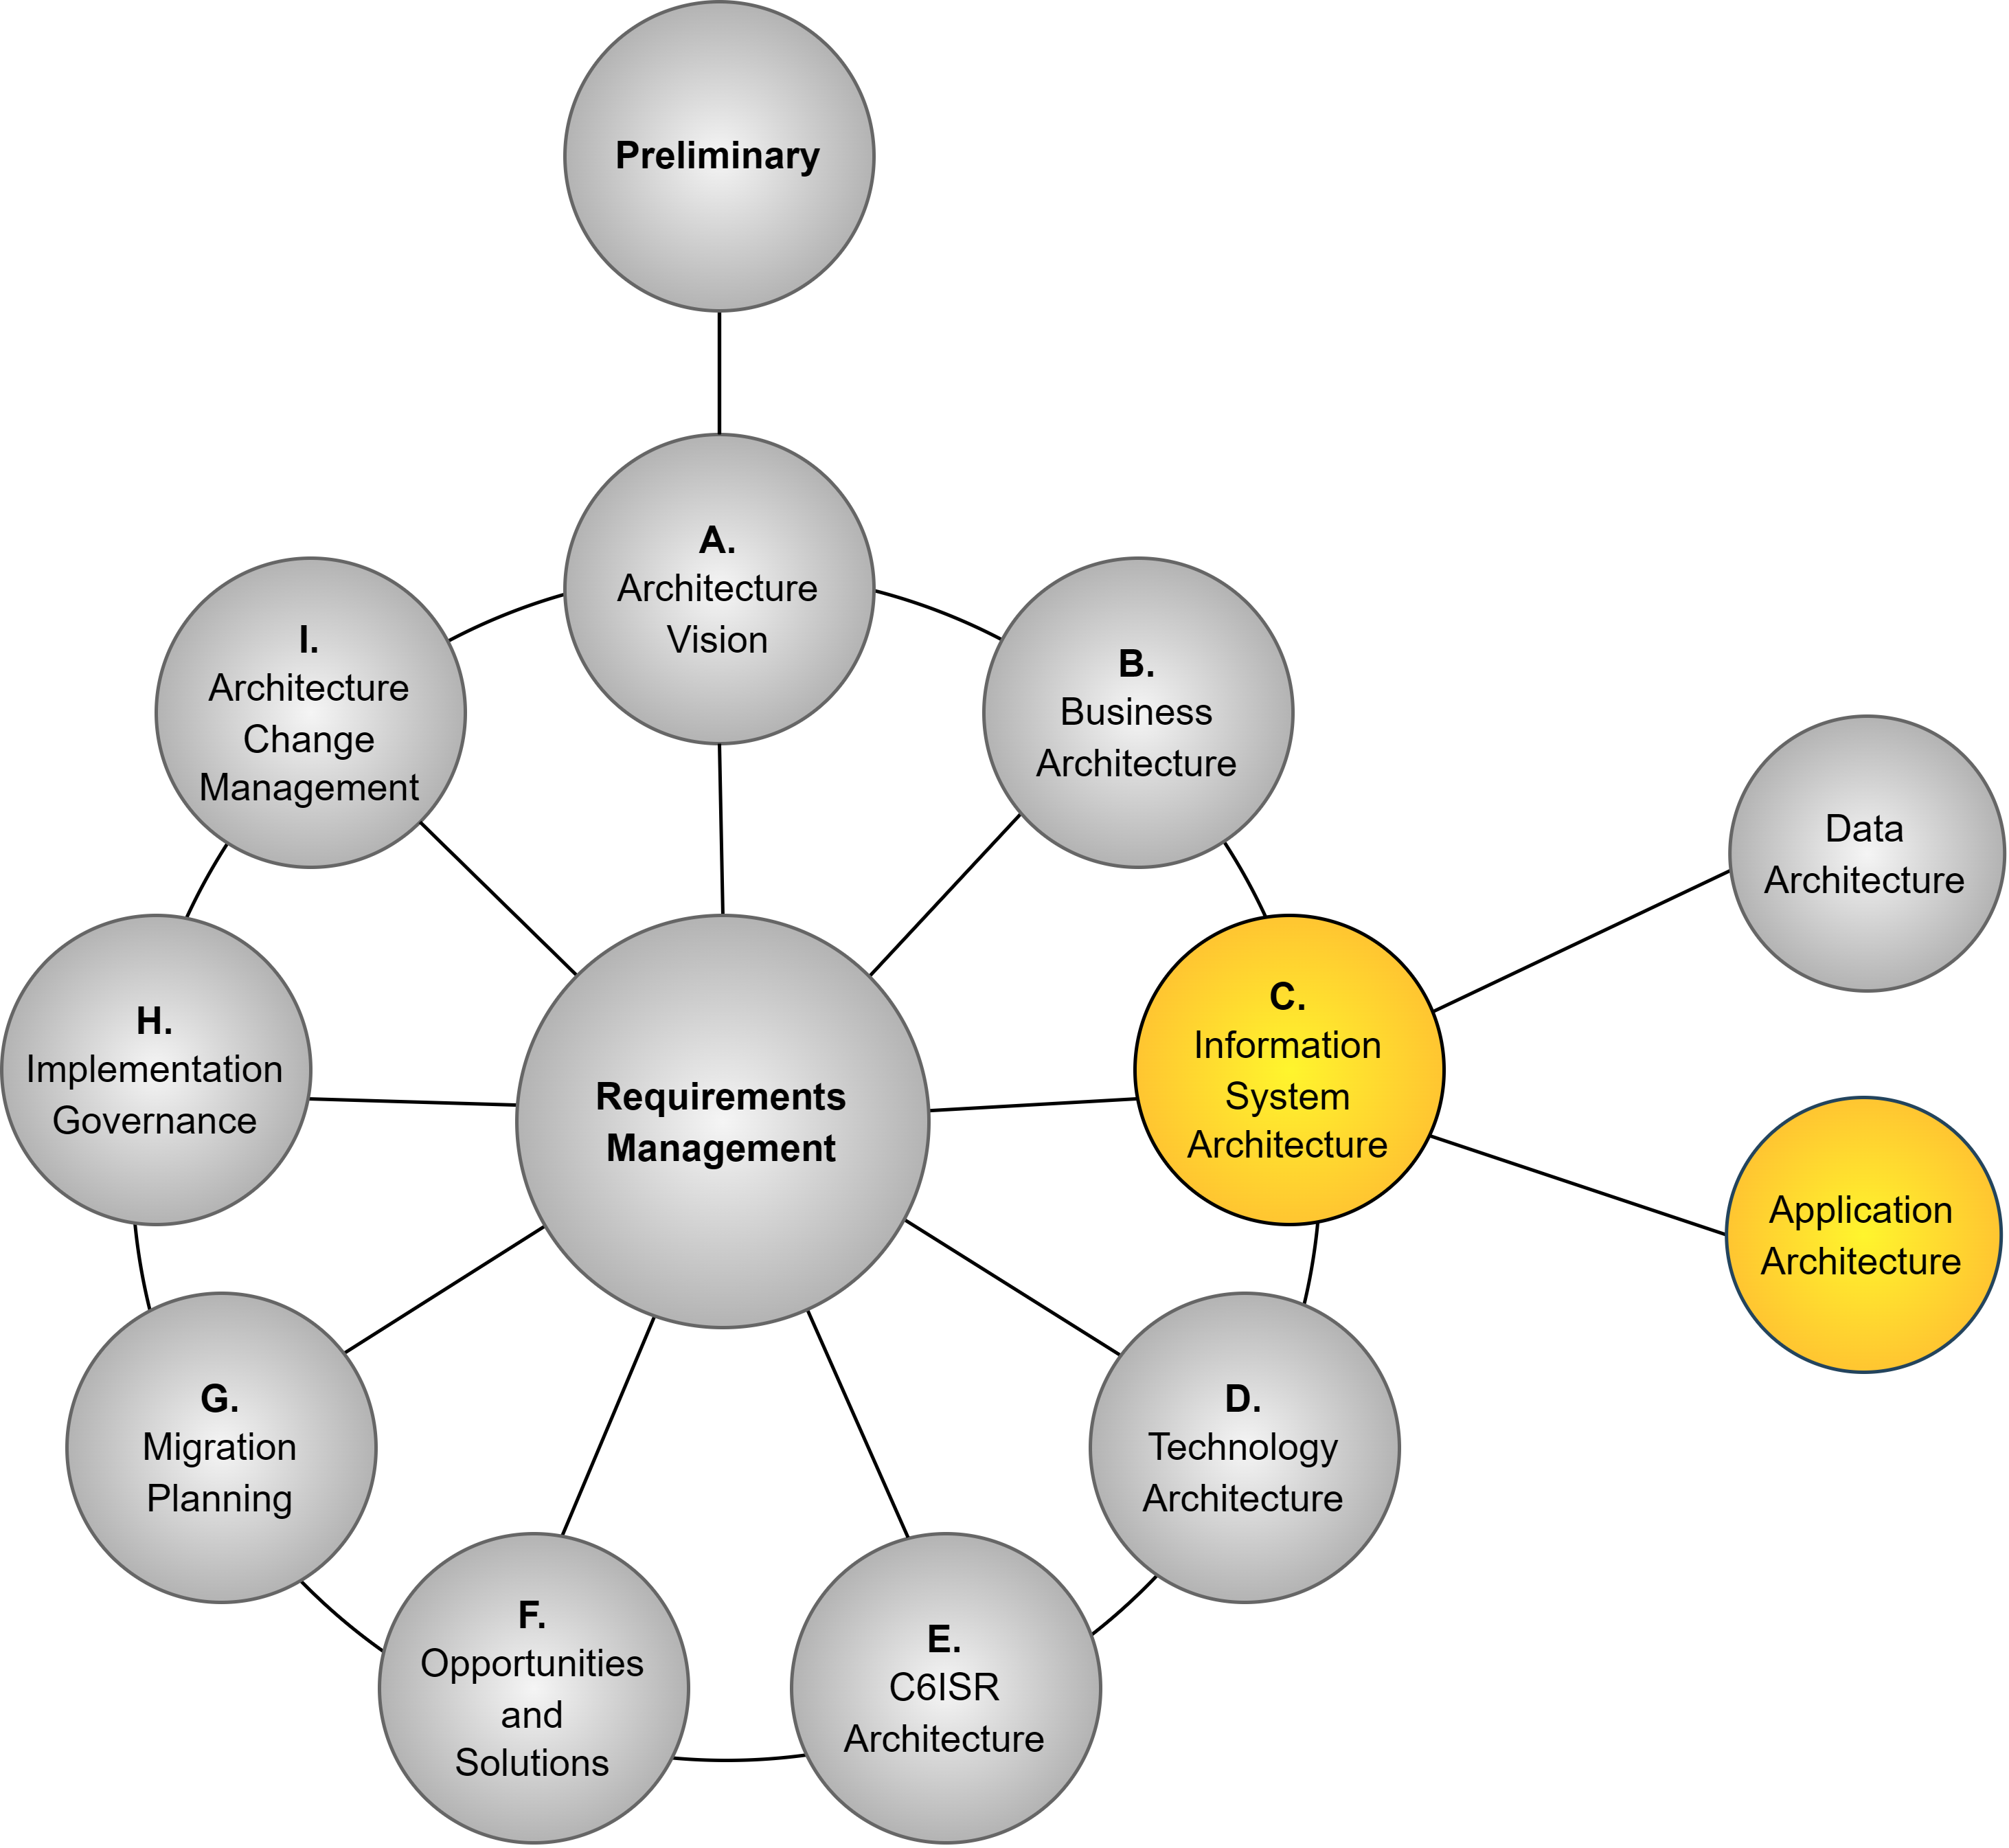
\includegraphics[width=0.61\linewidth,height=0.8\textheight,keepaspectratio]{images/Fase Application Architecture.drawio.png}
\caption{\textit{Application Architecture}}
\label{fig:III.7}
\end{figure}

Input, step, dan output \textit{Application Architecture} disajikan pada Tabel~\ref{tab:III.11}.

\begingroup\small\setstretch{1.0}
\begin{longtable}{@{}>{\raggedright\arraybackslash\hspace{0pt}}p{0.312\linewidth}>{\raggedright\arraybackslash\hspace{0pt}}p{0.312\linewidth}>{\raggedright\arraybackslash\hspace{0pt}}p{0.312\linewidth}@{}}
\caption{Input, Step, dan Output \textit{Application Architecture}}\label{tab:III.11}\\
\toprule
\textbf{INPUT} & \textbf{STEP} & \textbf{OUTPUT}\\
\midrule
\endfirsthead
\multicolumn{3}{@{}l}{\small\itshape \tablename\ \thetable{} (lanjutan)}\\
\toprule
\textbf{INPUT} & \textbf{STEP} & \textbf{OUTPUT}\\
\midrule
\endhead
\bottomrule
\endlastfoot
\hangindent=1.1em\hangafter=1 \makebox[1.1em][l]{1.}\textit{Statement of Architecture Work} dan dokumen \textit{Architecture Vision}\par \hangindent=1.1em\hangafter=1 \makebox[1.1em][l]{2.}Prinsip arsitektur Pertahanan Indonesia\par \hangindent=1.1em\hangafter=1 \makebox[1.1em][l]{3.}Komponen arsitektur bisnis dan data pada roadmap\par \hangindent=1.1em\hangafter=1 \makebox[1.1em][l]{4.}Inventaris aplikasi Kemhan RI\par \hangindent=1.1em\hangafter=1 \makebox[1.1em][l]{5.}Standar interoperabilitas dan integrasi lintas matra (+) & \hangindent=1.1em\hangafter=1 \makebox[1.1em][l]{1.}Memilih model rujukan, viewpoint, dan perangkat pemodelan aplikasi\par \hangindent=1.1em\hangafter=1 \makebox[1.1em][l]{2.}Menyusun arsitektur aplikasi baseline melalui inventarisasi aplikasi\par \hangindent=1.1em\hangafter=1 \makebox[1.1em][l]{3.}Menyusun arsitektur aplikasi target\par \hangindent=1.1em\hangafter=1 \makebox[1.1em][l]{4.}Merancang portofolio aplikasi dan rasionalisasinya\par \hangindent=1.1em\hangafter=1 \makebox[1.1em][l]{5.}Merancang integrasi dan pertukaran data lintas matra (Δ)\par \hangindent=1.1em\hangafter=1 \makebox[1.1em][l]{6.}Melakukan analisis kesenjangan dan menetapkan komponen \textit{roadmap} & \hangindent=1.1em\hangafter=1 \makebox[1.1em][l]{1.}Portofolio aplikasi target\par \hangindent=1.1em\hangafter=1 \makebox[1.1em][l]{2.}Peta keterkaitan aplikasi dengan kapabilitas dan proses bisnis\par \hangindent=1.1em\hangafter=1 \makebox[1.1em][l]{3.}Daftar aplikasi yang dipertahankan, digabungkan, atau dihentikan\par \hangindent=1.1em\hangafter=1 \makebox[1.1em][l]{4.}Rancangan integrasi dan pertukaran data lintas matra (+)\par \hangindent=1.1em\hangafter=1 \makebox[1.1em][l]{5.}Komponen arsitektur aplikasi pada \textit{roadmap}\\
\end{longtable}
\endgroup

Keterangan: (+) = muatan baru; (Δ) = muatan TOGAF yang disesuaikan; tanpa tanda = TOGAF ADM standar.

Tabel~\ref{tab:III.11} menunjukkan bahwa subdomain ini berorientasi pada rasionalisasi aplikasi.

\subsection{Fase \textit{Technology Architecture}}
\label{sec:III.3.5}

Fase Technology Architecture merancang infrastruktur jaringan, pusat data, komputasi awan, serta lapisan keamanan siber yang menjadi fondasi ekosistem digital pertahanan. Kedudukan fase ini ditunjukkan pada Gambar~\ref{fig:III.8}.
\begin{figure}[htbp]
\centering
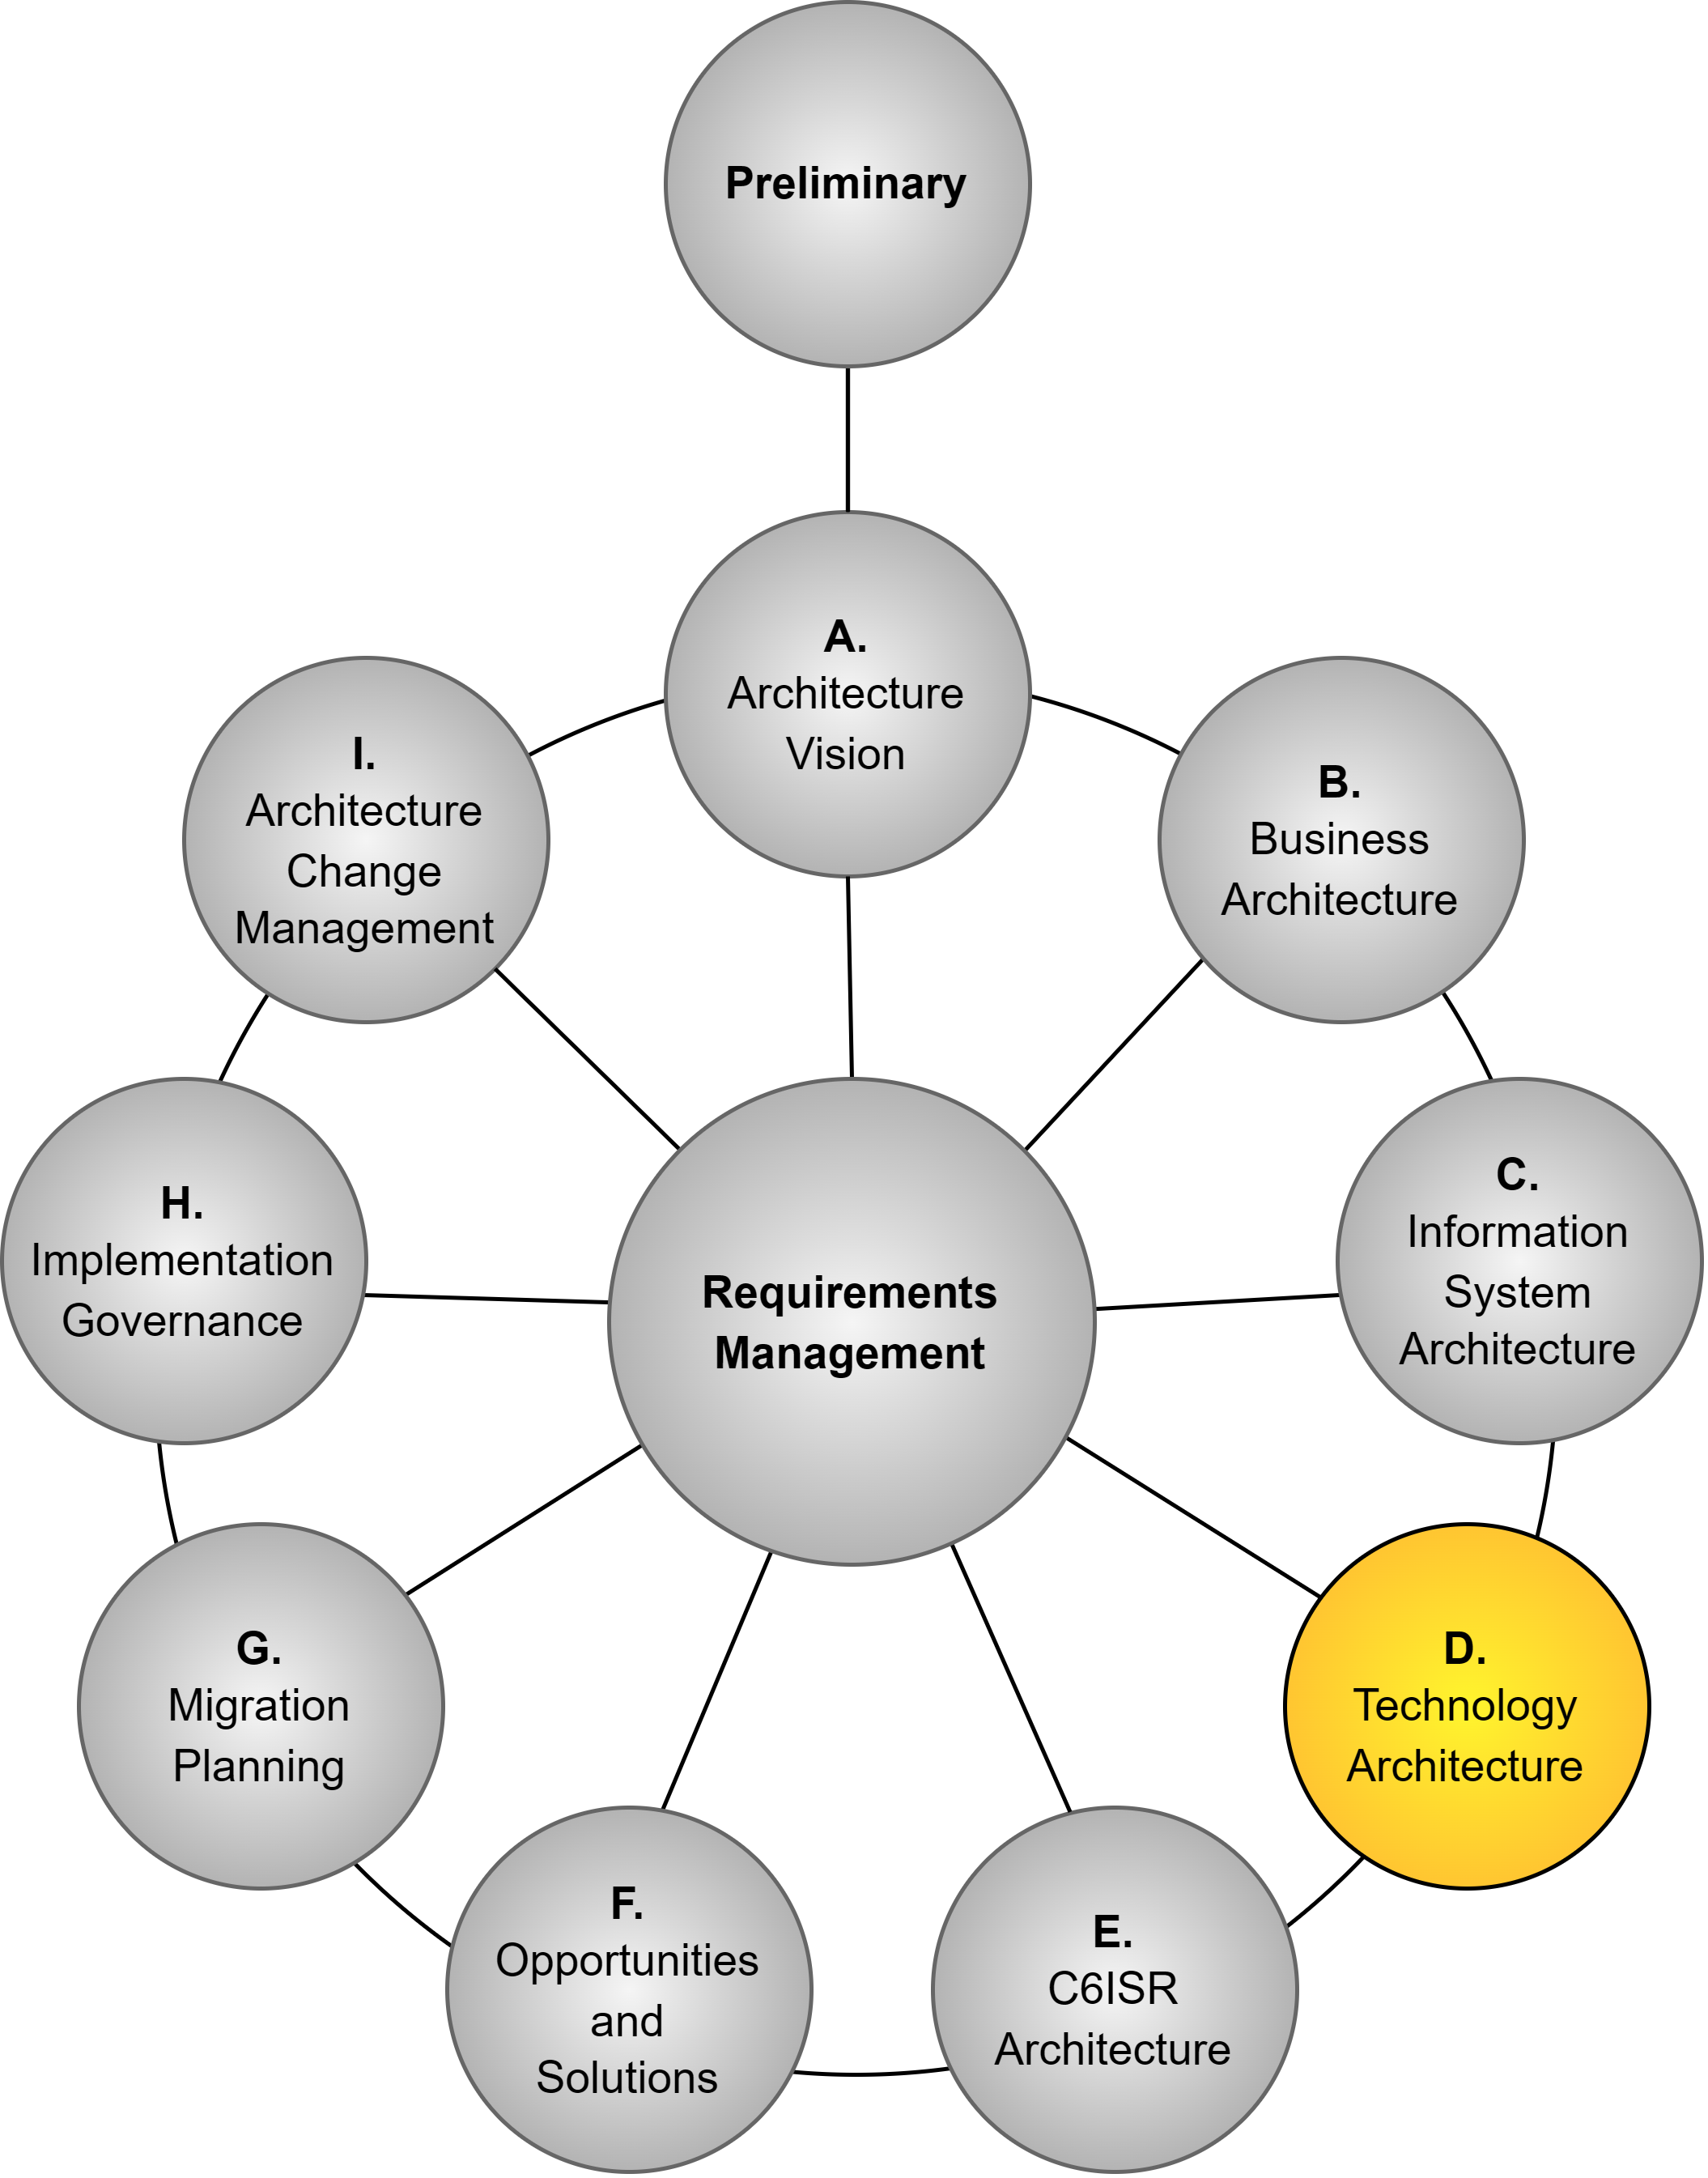
\includegraphics[width=0.46\linewidth,height=0.8\textheight,keepaspectratio]{images/Fase Technology Architecture.drawio.png}
\caption{Fase \textit{Technology Architecture}}
\label{fig:III.8}
\end{figure}

Input, step, dan output Fase \textit{Technology Architecture} disajikan pada Tabel~\ref{tab:III.12}.

\begingroup\small\setstretch{1.0}
\begin{longtable}{@{}>{\raggedright\arraybackslash\hspace{0pt}}p{0.312\linewidth}>{\raggedright\arraybackslash\hspace{0pt}}p{0.312\linewidth}>{\raggedright\arraybackslash\hspace{0pt}}p{0.312\linewidth}@{}}
\caption{Input, Step, dan Output Fase \textit{Technology Architecture}}\label{tab:III.12}\\
\toprule
\textbf{INPUT} & \textbf{STEP} & \textbf{OUTPUT}\\
\midrule
\endfirsthead
\multicolumn{3}{@{}l}{\small\itshape \tablename\ \thetable{} (lanjutan)}\\
\toprule
\textbf{INPUT} & \textbf{STEP} & \textbf{OUTPUT}\\
\midrule
\endhead
\bottomrule
\endlastfoot
\hangindent=1.1em\hangafter=1 \makebox[1.1em][l]{1.}\textit{Statement of Architecture Work} dan dokumen \textit{Architecture Vision}\par \hangindent=1.1em\hangafter=1 \makebox[1.1em][l]{2.}Prinsip arsitektur Pertahanan Indonesia\par \hangindent=1.1em\hangafter=1 \makebox[1.1em][l]{3.}Komponen arsitektur data dan aplikasi\par \hangindent=1.1em\hangafter=1 \makebox[1.1em][l]{4.}Spesifikasi produk teknologi yang dipertimbangkan untuk digunakan\par \hangindent=1.1em\hangafter=1 \makebox[1.1em][l]{5.}Kebutuhan keamanan siber pertahanan (+) & \hangindent=1.1em\hangafter=1 \makebox[1.1em][l]{1.}Memilih model rujukan, \textit{viewpoint}, dan perangkat pemodelan\par \hangindent=1.1em\hangafter=1 \makebox[1.1em][l]{2.}Menyusun arsitektur teknologi baseline\par \hangindent=1.1em\hangafter=1 \makebox[1.1em][l]{3.}Menetapkan prinsip dan standar teknologi (Δ)\par \hangindent=1.1em\hangafter=1 \makebox[1.1em][l]{4.}Menyusun arsitektur teknologi target yang mencakup jaringan, \textit{server}, \textit{cloud}, dan \textit{edge}\par \hangindent=1.1em\hangafter=1 \makebox[1.1em][l]{5.}Merancang lapisan keamanan siber terpadu (+)\par \hangindent=1.1em\hangafter=1 \makebox[1.1em][l]{6.}Melakukan analisis kesenjangan dan menetapkan komponen roadmap\par \hangindent=1.1em\hangafter=1 \makebox[1.1em][l]{7.}Memfinalkan arsitektur teknologi & \hangindent=1.1em\hangafter=1 \makebox[1.1em][l]{1.}Arsitektur teknologi target\par \hangindent=1.1em\hangafter=1 \makebox[1.1em][l]{2.}Standar teknologi dan protokol keamanan (Δ)\par \hangindent=1.1em\hangafter=1 \makebox[1.1em][l]{3.}Rancangan lapisan keamanan siber terpadu (+)\par \hangindent=1.1em\hangafter=1 \makebox[1.1em][l]{4.}Komponen teknologi pada roadmap\par \hangindent=1.1em\hangafter=1 \makebox[1.1em][l]{5.}Pemutakhiran \textit{Architecture Definition Document} dan \textit{Architecture Requirements Specification}\\
\end{longtable}
\endgroup

Keterangan: (+) = muatan baru; (Δ) = muatan TOGAF yang disesuaikan; tanpa tanda = TOGAF ADM standar.

Tabel~\ref{tab:III.12} menunjukkan bahwa kebutuhan keamanan siber merupakan input fase ini, sesuai prinsip \textit{Security by Design}.

\subsection{Fase \textit{C6ISR Architecture}}
\label{sec:III.3.6}

Fase C6ISR Architecture merupakan fase baru pada TOGAF Pertahanan Indonesia. Fase ini merancang kapabilitas C6ISR yang mengintegrasikan ISR, komando-kendali, dan unsur penindak dalam satu jaringan informasi terpadu, dengan keluaran Fase B, C, dan D sebagai fondasinya. Kedudukan fase ini ditunjukkan pada Gambar~\ref{fig:III.9}.
\begin{figure}[htbp]
\centering
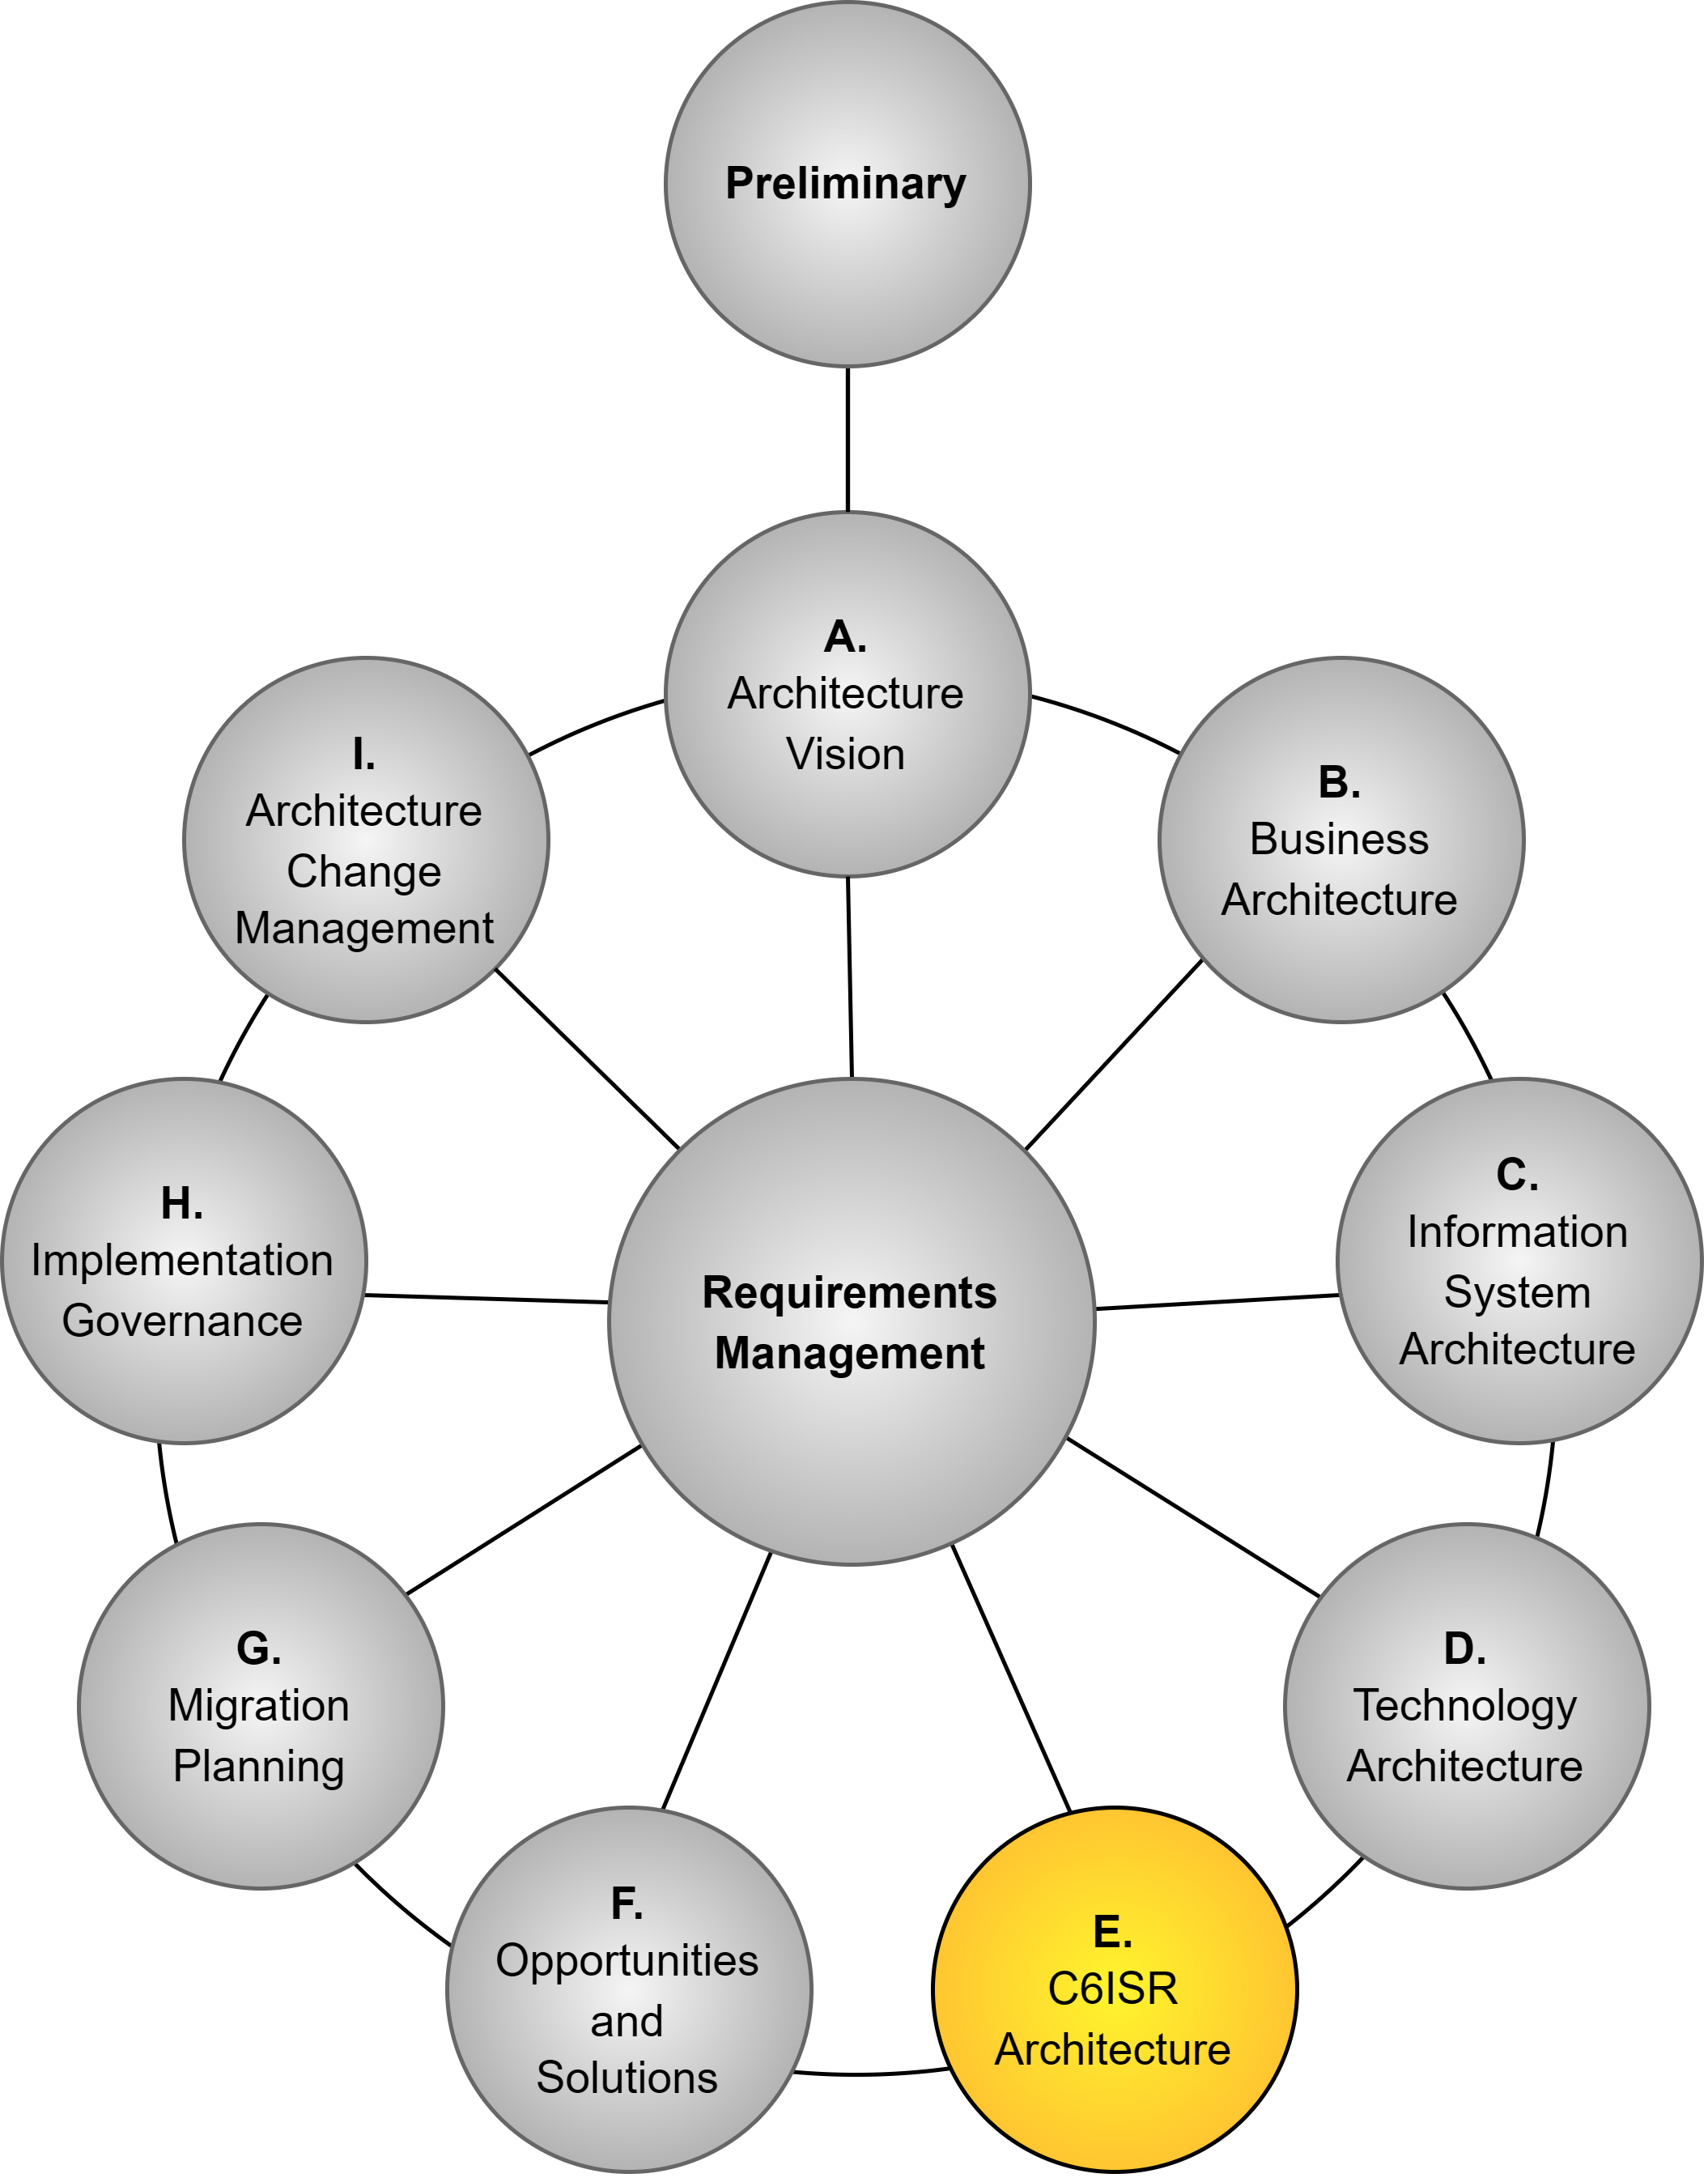
\includegraphics[width=0.46\linewidth,height=0.8\textheight,keepaspectratio]{images/Fase C6ISR Architecture.drawio.png}
\caption{Fase \textit{C6ISR Architecture}}
\label{fig:III.9}
\end{figure}

Input, step, dan output Fase \textit{C6ISR Architecture} disajikan pada Tabel~\ref{tab:III.13}.

\begingroup\small\setstretch{1.0}
\begin{longtable}{@{}>{\raggedright\arraybackslash\hspace{0pt}}p{0.312\linewidth}>{\raggedright\arraybackslash\hspace{0pt}}p{0.312\linewidth}>{\raggedright\arraybackslash\hspace{0pt}}p{0.312\linewidth}@{}}
\caption{Input, Step, dan Output Fase \textit{C6ISR Architecture}}\label{tab:III.13}\\
\toprule
\textbf{INPUT} & \textbf{STEP} & \textbf{OUTPUT}\\
\midrule
\endfirsthead
\multicolumn{3}{@{}l}{\small\itshape \tablename\ \thetable{} (lanjutan)}\\
\toprule
\textbf{INPUT} & \textbf{STEP} & \textbf{OUTPUT}\\
\midrule
\endhead
\bottomrule
\endlastfoot
\hangindent=1.1em\hangafter=1 \makebox[1.1em][l]{1.}Model tata kelola dan komando serta model interoperabilitas lintas matra dari Fase B\par \hangindent=1.1em\hangafter=1 \makebox[1.1em][l]{2.}Arsitektur data dan aplikasi dari Fase C\par \hangindent=1.1em\hangafter=1 \makebox[1.1em][l]{3.}Arsitektur teknologi dan lapisan keamanan siber dari Fase D\par \hangindent=1.1em\hangafter=1 \makebox[1.1em][l]{4.}Prinsip \textit{Integrated Command \& Control} dan \textit{Interoperability}\par \hangindent=1.1em\hangafter=1 \makebox[1.1em][l]{5.}Doktrin pertahanan, konsep NCW, dan operasi multidomain\par \hangindent=1.1em\hangafter=1 \makebox[1.1em][l]{6.}Standar interoperabilitas lintas matra dan \textit{concern} NAF & \hangindent=1.1em\hangafter=1 \makebox[1.1em][l]{1.}Mengidentifikasi kebutuhan operasional\par \hangindent=1.1em\hangafter=1 \makebox[1.1em][l]{2.}Menyusun arsitektur C6ISR baseline\par \hangindent=1.1em\hangafter=1 \makebox[1.1em][l]{3.}Menyusun peta kapabilitas C6ISR\par \hangindent=1.1em\hangafter=1 \makebox[1.1em][l]{4.}Merancang arsitektur target per lapisan, yaitu \textit{command \& control}, \textit{computers}, \textit{communications}, \textit{cyber-defense, combat systems}, dan ISR\par \hangindent=1.1em\hangafter=1 \makebox[1.1em][l]{5.}Merancang skema komunikasi PACE\par \hangindent=1.1em\hangafter=1 \makebox[1.1em][l]{6.}Mengintegrasikan ISR, komando-kendali, dan unsur penindak dalam satu jaringan\par \hangindent=1.1em\hangafter=1 \makebox[1.1em][l]{7.}Melakukan analisis kesenjangan dan menetapkan komponen roadmap & \hangindent=1.1em\hangafter=1 \makebox[1.1em][l]{1.}Kebutuhan operasional C6ISR\par \hangindent=1.1em\hangafter=1 \makebox[1.1em][l]{2.}Arsitektur C6ISR baseline\par \hangindent=1.1em\hangafter=1 \makebox[1.1em][l]{3.}Peta kapabilitas C6ISR\par \hangindent=1.1em\hangafter=1 \makebox[1.1em][l]{4.}Arsitektur C6ISR target per lapisan\par \hangindent=1.1em\hangafter=1 \makebox[1.1em][l]{5.}Analisis kesenjangan C6ISR\par \hangindent=1.1em\hangafter=1 \makebox[1.1em][l]{6.}Komponen C6ISR pada roadmap\par \hangindent=1.1em\hangafter=1 \makebox[1.1em][l]{7.}Pemutakhiran \textit{Architecture Definition Document} dan \textit{Architecture Requirements Specification}\\
\end{longtable}
\endgroup

Keterangan: seluruh muatan fase ini merupakan muatan baru (+).

Tabel~\ref{tab:III.13} menunjukkan bahwa fase ini disusun dengan pola yang sama dengan fase arsitektur lainnya, sehingga keluarannya dapat dikonsolidasikan pada Fase \textit{Opportunities \& Solutions}.

\subsection{Fase \textit{Opportunities \& Solutions}}
\label{sec:III.3.7}

Fase \textit{Opportunities \& Solutions} mengonsolidasikan kesenjangan dari Fase B hingga Fase E menjadi paket pekerjaan dan arsitektur transisi. Fase ini menjadi penghubung antara fase perancangan dan fase realisasi. Kedudukan fase ini ditunjukkan pada Gambar~\ref{fig:III.10}.
\begin{figure}[htbp]
\centering
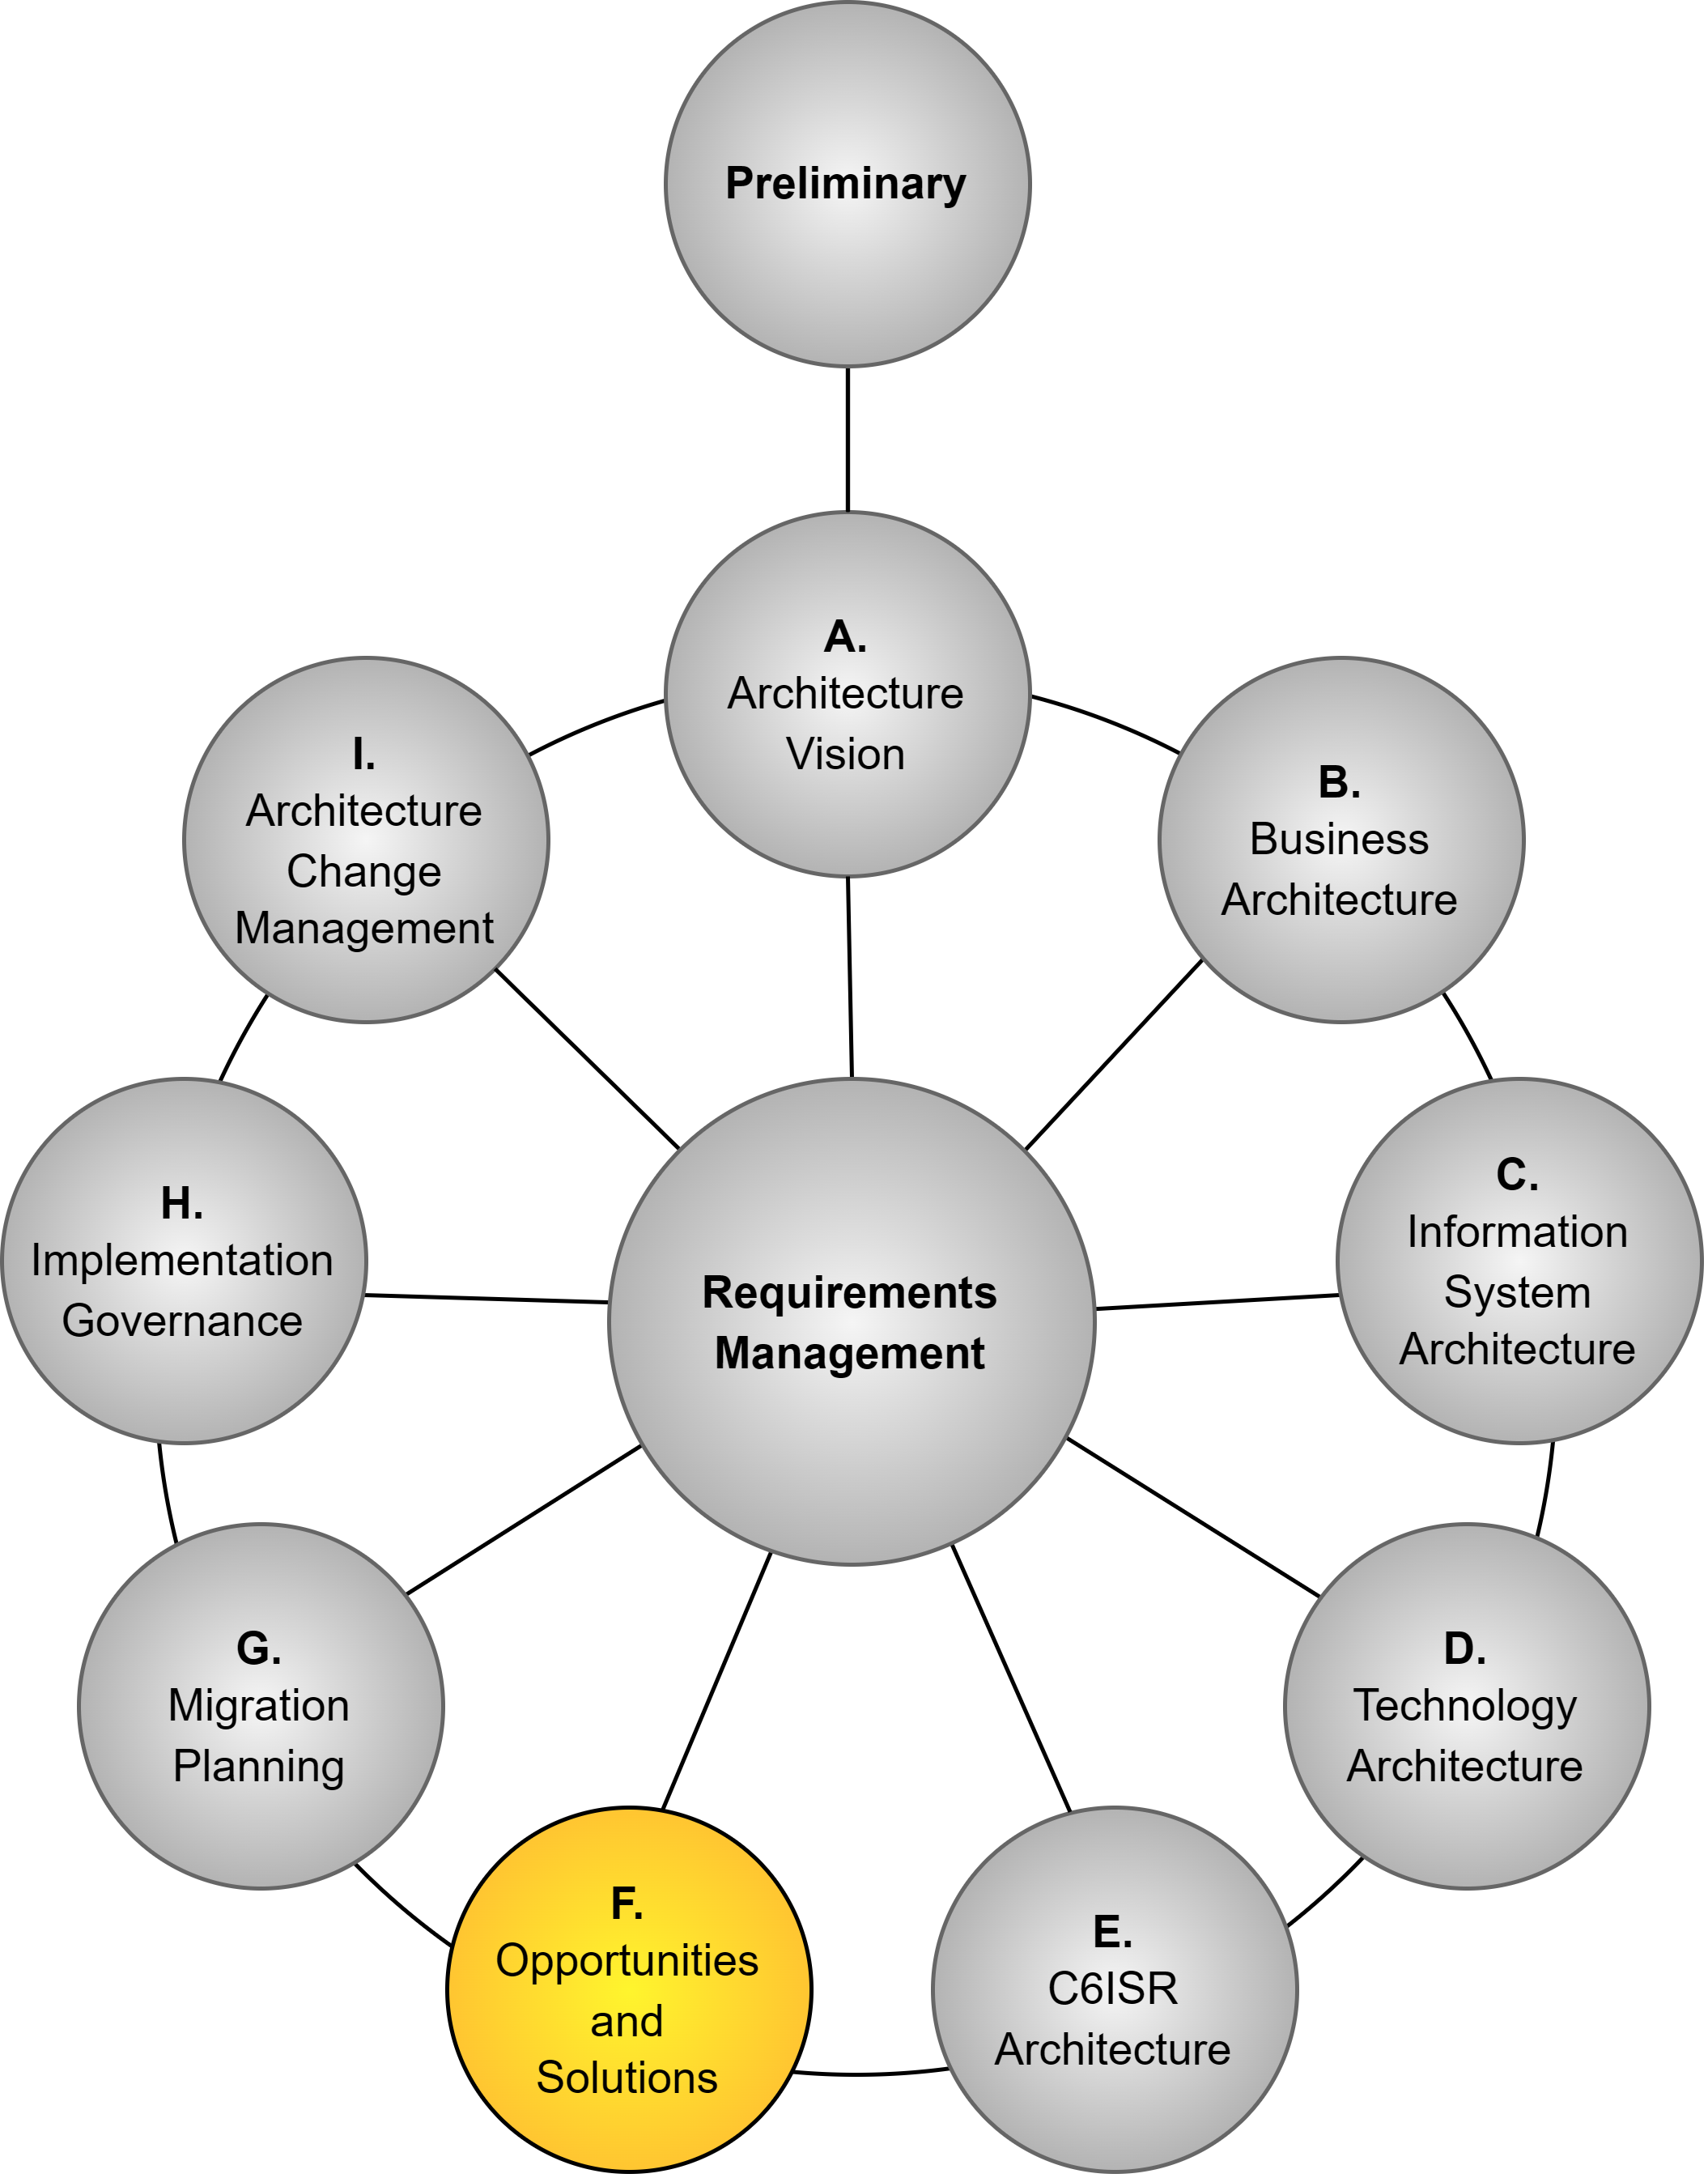
\includegraphics[width=0.46\linewidth,height=0.8\textheight,keepaspectratio]{images/Fase Opportunities and Solutions.drawio.png}
\caption{Fase \textit{Opportunities \& Solutions}}
\label{fig:III.10}
\end{figure}

Input, step, dan output Fase \textit{Opportunities \& Solutions} disajikan pada Tabel~\ref{tab:III.14}.

\begingroup\small\setstretch{1.0}
\begin{longtable}{@{}>{\raggedright\arraybackslash\hspace{0pt}}p{0.312\linewidth}>{\raggedright\arraybackslash\hspace{0pt}}p{0.312\linewidth}>{\raggedright\arraybackslash\hspace{0pt}}p{0.312\linewidth}@{}}
\caption{Input, Step, dan Output Fase \textit{Opportunities \& Solutions}}\label{tab:III.14}\\
\toprule
\textbf{INPUT} & \textbf{STEP} & \textbf{OUTPUT}\\
\midrule
\endfirsthead
\multicolumn{3}{@{}l}{\small\itshape \tablename\ \thetable{} (lanjutan)}\\
\toprule
\textbf{INPUT} & \textbf{STEP} & \textbf{OUTPUT}\\
\midrule
\endhead
\bottomrule
\endlastfoot
\hangindent=1.1em\hangafter=1 \makebox[1.1em][l]{1.}Hasil analisis kesenjangan Fase B hingga Fase E\par \hangindent=1.1em\hangafter=1 \makebox[1.1em][l]{2.}Komponen roadmap dari setiap domain\par \hangindent=1.1em\hangafter=1 \makebox[1.1em][l]{3.}\textit{Draf Architecture Definition Document} dan \textit{Architecture Requirements Specification}\par \hangindent=1.1em\hangafter=1 \makebox[1.1em][l]{4.}Hasil penilaian kapabilitas\par \hangindent=1.1em\hangafter=1 \makebox[1.1em][l]{5.}Prinsip arsitektur dan prioritas strategis organisasi & \hangindent=1.1em\hangafter=1 \makebox[1.1em][l]{1.}Menetapkan atribut perubahan dan kendala implementasi\par \hangindent=1.1em\hangafter=1 \makebox[1.1em][l]{2.}Mengonsolidasikan kesenjangan lintas domain\par \hangindent=1.1em\hangafter=1 \makebox[1.1em][l]{3.}Menyelaraskan kebutuhan interoperabilitas lintas matra\par \hangindent=1.1em\hangafter=1 \makebox[1.1em][l]{4.}Merumuskan paket pekerjaan dan ketergantungannya\par \hangindent=1.1em\hangafter=1 \makebox[1.1em][l]{5.}Menilai kesiapan dan risiko implementasi\par \hangindent=1.1em\hangafter=1 \makebox[1.1em][l]{6.}Menyusun strategi implementasi dan arsitektur transisi\par \hangindent=1.1em\hangafter=1 \makebox[1.1em][l]{7.}Menyusun roadmap arsitektur & \hangindent=1.1em\hangafter=1 \makebox[1.1em][l]{1.}Daftar paket pekerjaan dan inisiatif transformasi\par \hangindent=1.1em\hangafter=1 \makebox[1.1em][l]{2.}Arsitektur transisi\par \hangindent=1.1em\hangafter=1 \makebox[1.1em][l]{3.}Roadmap arsitektur\par \hangindent=1.1em\hangafter=1 \makebox[1.1em][l]{4.}Garis besar rencana implementasi dan migrasi\par \hangindent=1.1em\hangafter=1 \makebox[1.1em][l]{5.}Pemutakhiran \textit{Architecture Definition Document} dan \textit{Architecture Requirements Specification}\\
\end{longtable}
\endgroup

Keterangan: seluruh muatan mengikuti TOGAF ADM standar.

Tabel~\ref{tab:III.14} menunjukkan bahwa fase ini mengikuti TOGAF ADM standar. Perbedaannya hanya terletak pada cakupan kesenjangan yang turut memuat Fase C6ISR Architecture.

\subsection{Fase \textit{Migration Planning}}
\label{sec:III.3.8}

Fase Migration Planning menyusun rencana implementasi dan migrasi secara bertahap berdasarkan nilai manfaat, kebutuhan sumber daya, risiko, dan ketergantungan antarpaket pekerjaan. Kedudukan fase ini ditunjukkan pada Gambar~\ref{fig:III.11}.
\begin{figure}[htbp]
\centering
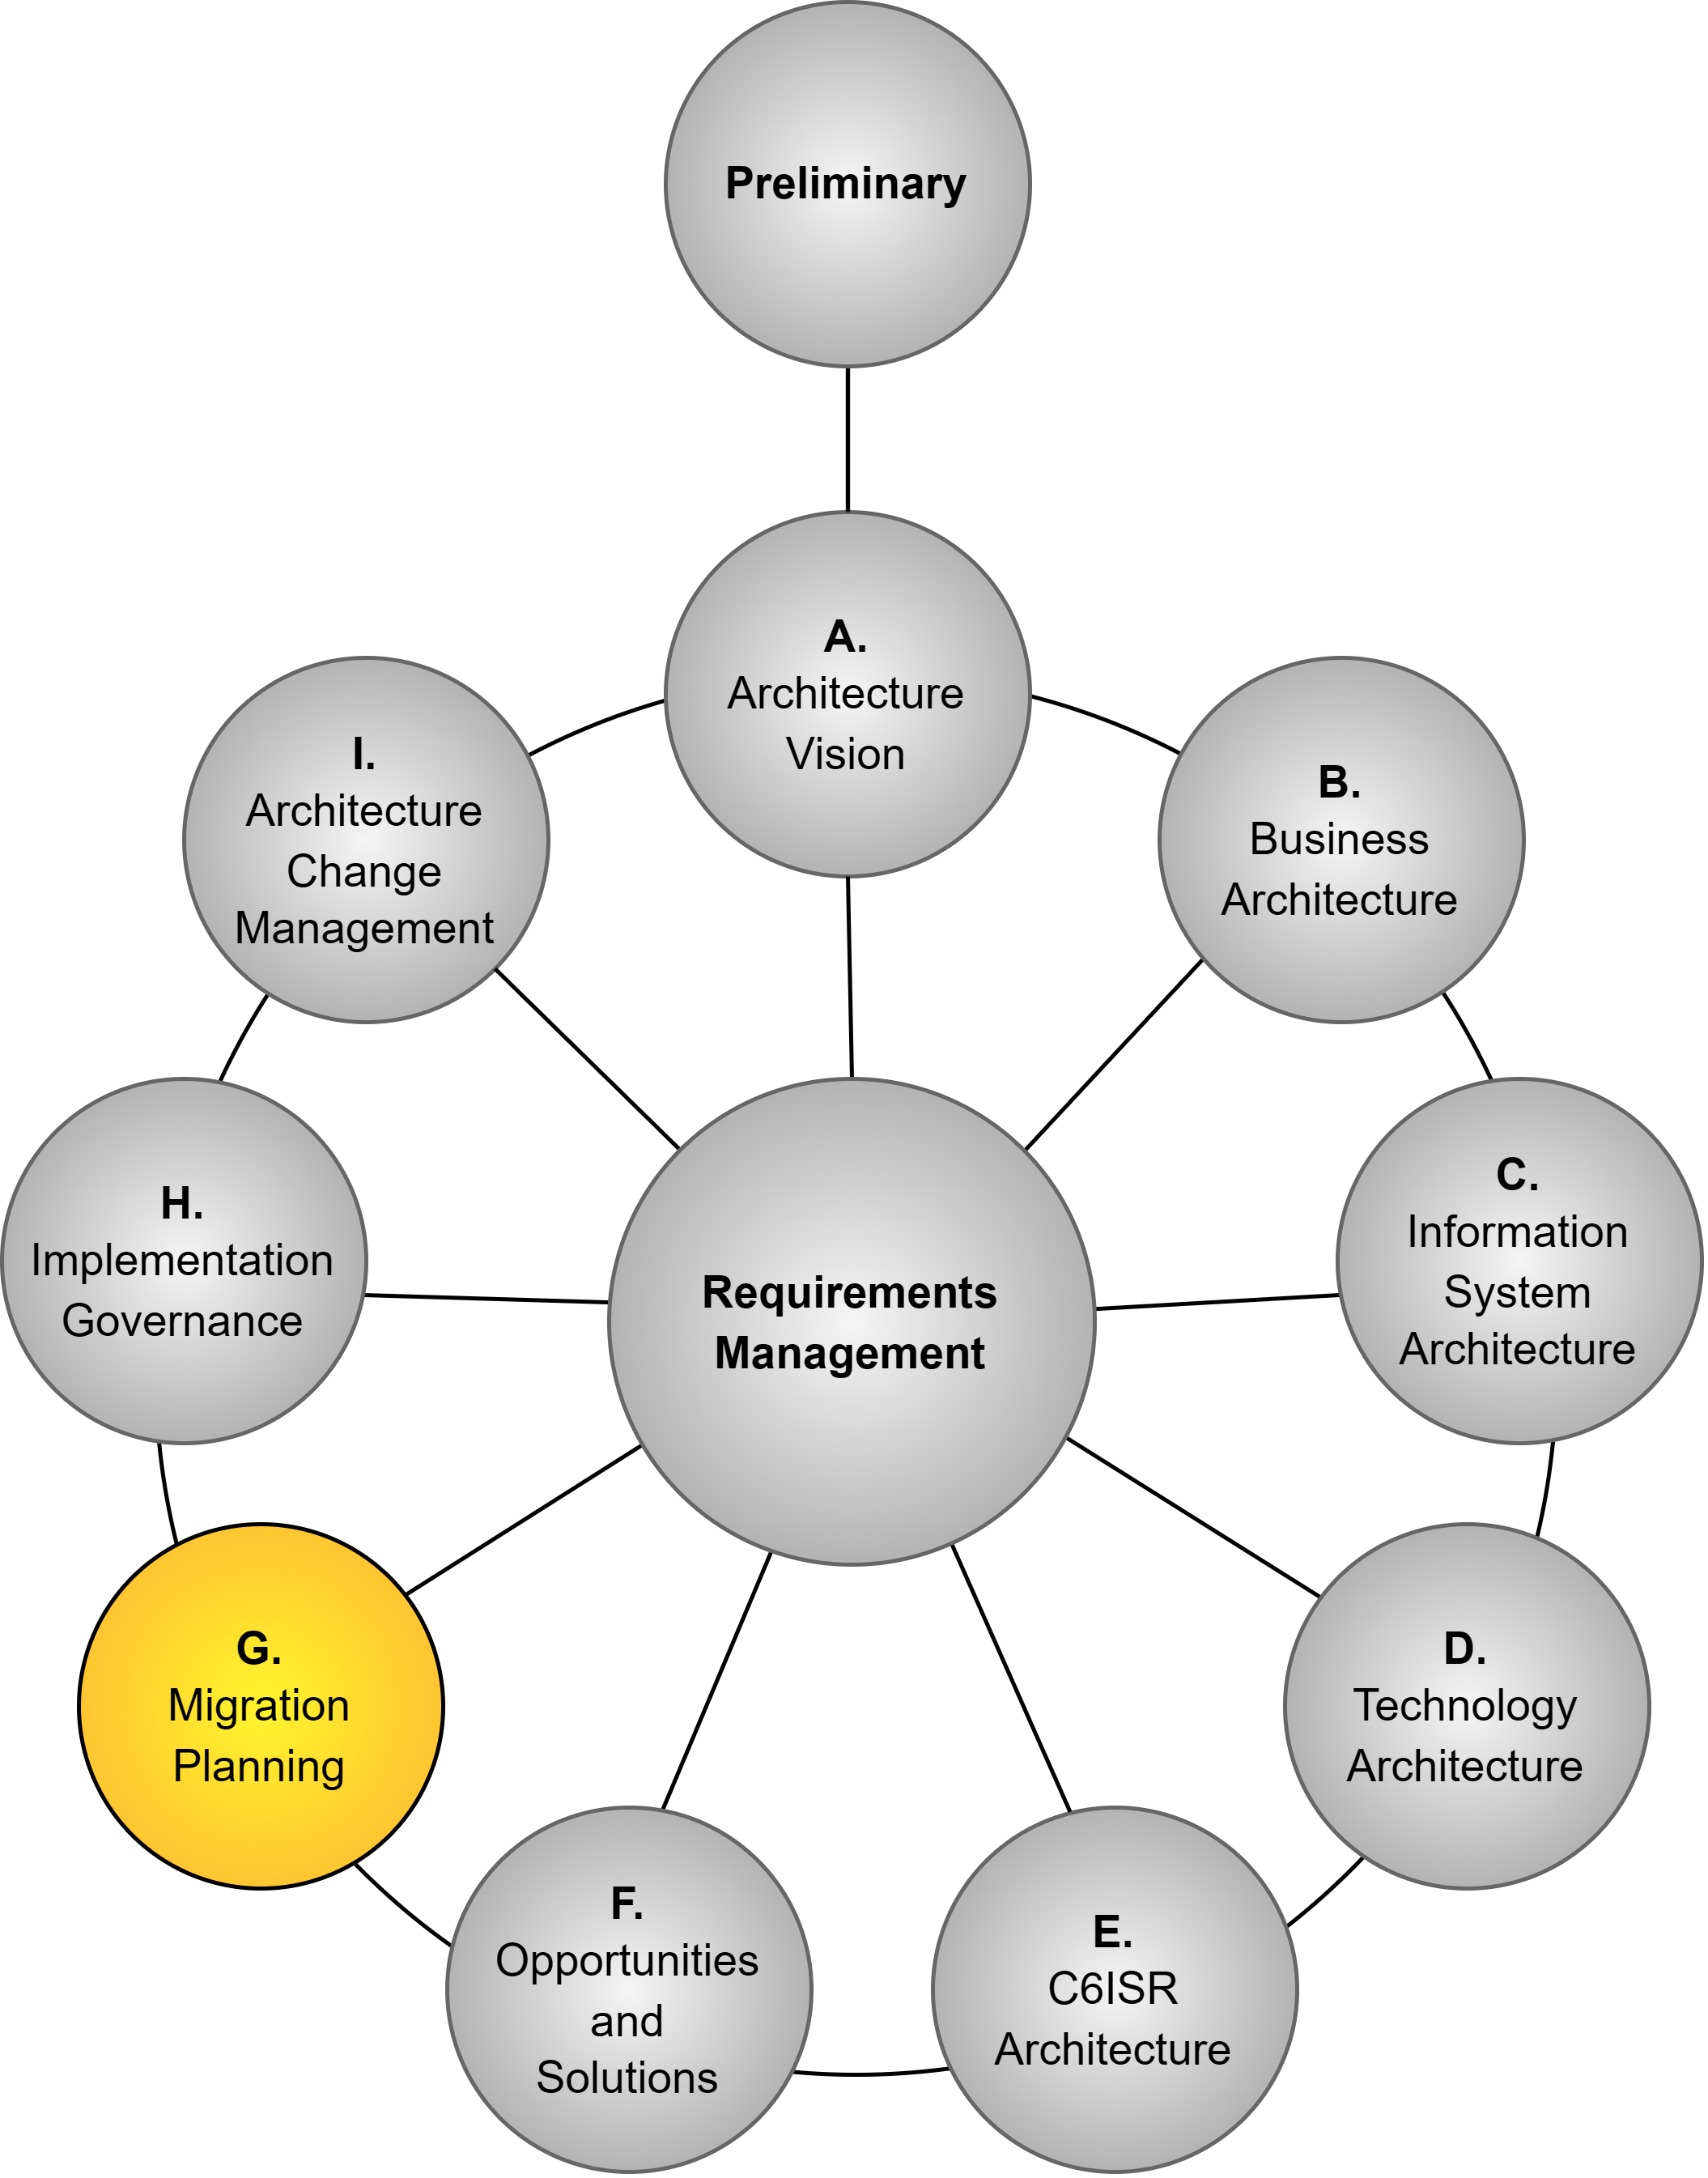
\includegraphics[width=0.46\linewidth,height=0.8\textheight,keepaspectratio]{images/Fase Migration Planning.drawio.png}
\caption{Fase \textit{Migration Planning}}
\label{fig:III.11}
\end{figure}

Input, step, dan output Fase \textit{Migration Planning} disajikan pada Tabel~\ref{tab:III.15}.

\begingroup\small\setstretch{1.0}
\begin{longtable}{@{}>{\raggedright\arraybackslash\hspace{0pt}}p{0.312\linewidth}>{\raggedright\arraybackslash\hspace{0pt}}p{0.312\linewidth}>{\raggedright\arraybackslash\hspace{0pt}}p{0.312\linewidth}@{}}
\caption{Input, Step, dan Output Fase \textit{Migration Planning}}\label{tab:III.15}\\
\toprule
\textbf{INPUT} & \textbf{STEP} & \textbf{OUTPUT}\\
\midrule
\endfirsthead
\multicolumn{3}{@{}l}{\small\itshape \tablename\ \thetable{} (lanjutan)}\\
\toprule
\textbf{INPUT} & \textbf{STEP} & \textbf{OUTPUT}\\
\midrule
\endhead
\bottomrule
\endlastfoot
\hangindent=1.1em\hangafter=1 \makebox[1.1em][l]{1.}Daftar paket pekerjaan dan arsitektur transisi\par \hangindent=1.1em\hangafter=1 \makebox[1.1em][l]{2.}\textit{Roadmap} arsitektur\par \hangindent=1.1em\hangafter=1 \makebox[1.1em][l]{3.}Garis besar rencana implementasi dan migrasi\par \hangindent=1.1em\hangafter=1 \makebox[1.1em][l]{4.}\textit{Draf Architecture Definition Document} dan \textit{Architecture Requirements Specification}\par \hangindent=1.1em\hangafter=1 \makebox[1.1em][l]{5.}Hasil penilaian kapabilitas & \hangindent=1.1em\hangafter=1 \makebox[1.1em][l]{1.}Mengonfirmasi keterkaitan rencana dengan kerangka manajemen organisasi\par \hangindent=1.1em\hangafter=1 \makebox[1.1em][l]{2.}Menetapkan model tata kelola implementasi\par \hangindent=1.1em\hangafter=1 \makebox[1.1em][l]{3.}Menilai nilai manfaat dan kebutuhan sumber daya\par \hangindent=1.1em\hangafter=1 \makebox[1.1em][l]{4.}Menetapkan prioritas paket pekerjaan\par \hangindent=1.1em\hangafter=1 \makebox[1.1em][l]{5.}Menyusun rencana implementasi dan migrasi bertahap beserta indikator keberhasilan\par \hangindent=1.1em\hangafter=1 \makebox[1.1em][l]{6.}Memfinalkan \textit{roadmap} dan \textit{Architecture Definition Document} & \hangindent=1.1em\hangafter=1 \makebox[1.1em][l]{1.}Rencana implementasi dan migrasi\par \hangindent=1.1em\hangafter=1 \makebox[1.1em][l]{2.}\textit{Roadmap} implementasi bertahap\par \hangindent=1.1em\hangafter=1 \makebox[1.1em][l]{3.}\textit{Architecture Definition Document} dan \textit{Architecture Requirements Specification final}\par \hangindent=1.1em\hangafter=1 \makebox[1.1em][l]{4.}Model tata kelola implementasi\par \hangindent=1.1em\hangafter=1 \makebox[1.1em][l]{5.}Kontrak arsitektur\par \hangindent=1.1em\hangafter=1 \makebox[1.1em][l]{6.}\textit{Request for Architecture Work} untuk siklus berikutnya\\
\end{longtable}
\endgroup

Keterangan: seluruh muatan mengikuti TOGAF ADM standar.

Tabel~\ref{tab:III.15} menunjukkan bahwa fase ini mengikuti TOGAF ADM. Keluarannya berupa roadmap implementasi.

\subsection{Fase \textit{Implementation Governance}}
\label{sec:III.3.9}

Fase Implementation Governance memastikan implementasi berjalan sesuai dengan arsitektur serta patuh terhadap regulasi nasional dan ketentuan sektor pertahanan. Kedudukan fase ini ditunjukkan pada Gambar~\ref{fig:III.12}.
\begin{figure}[htbp]
\centering
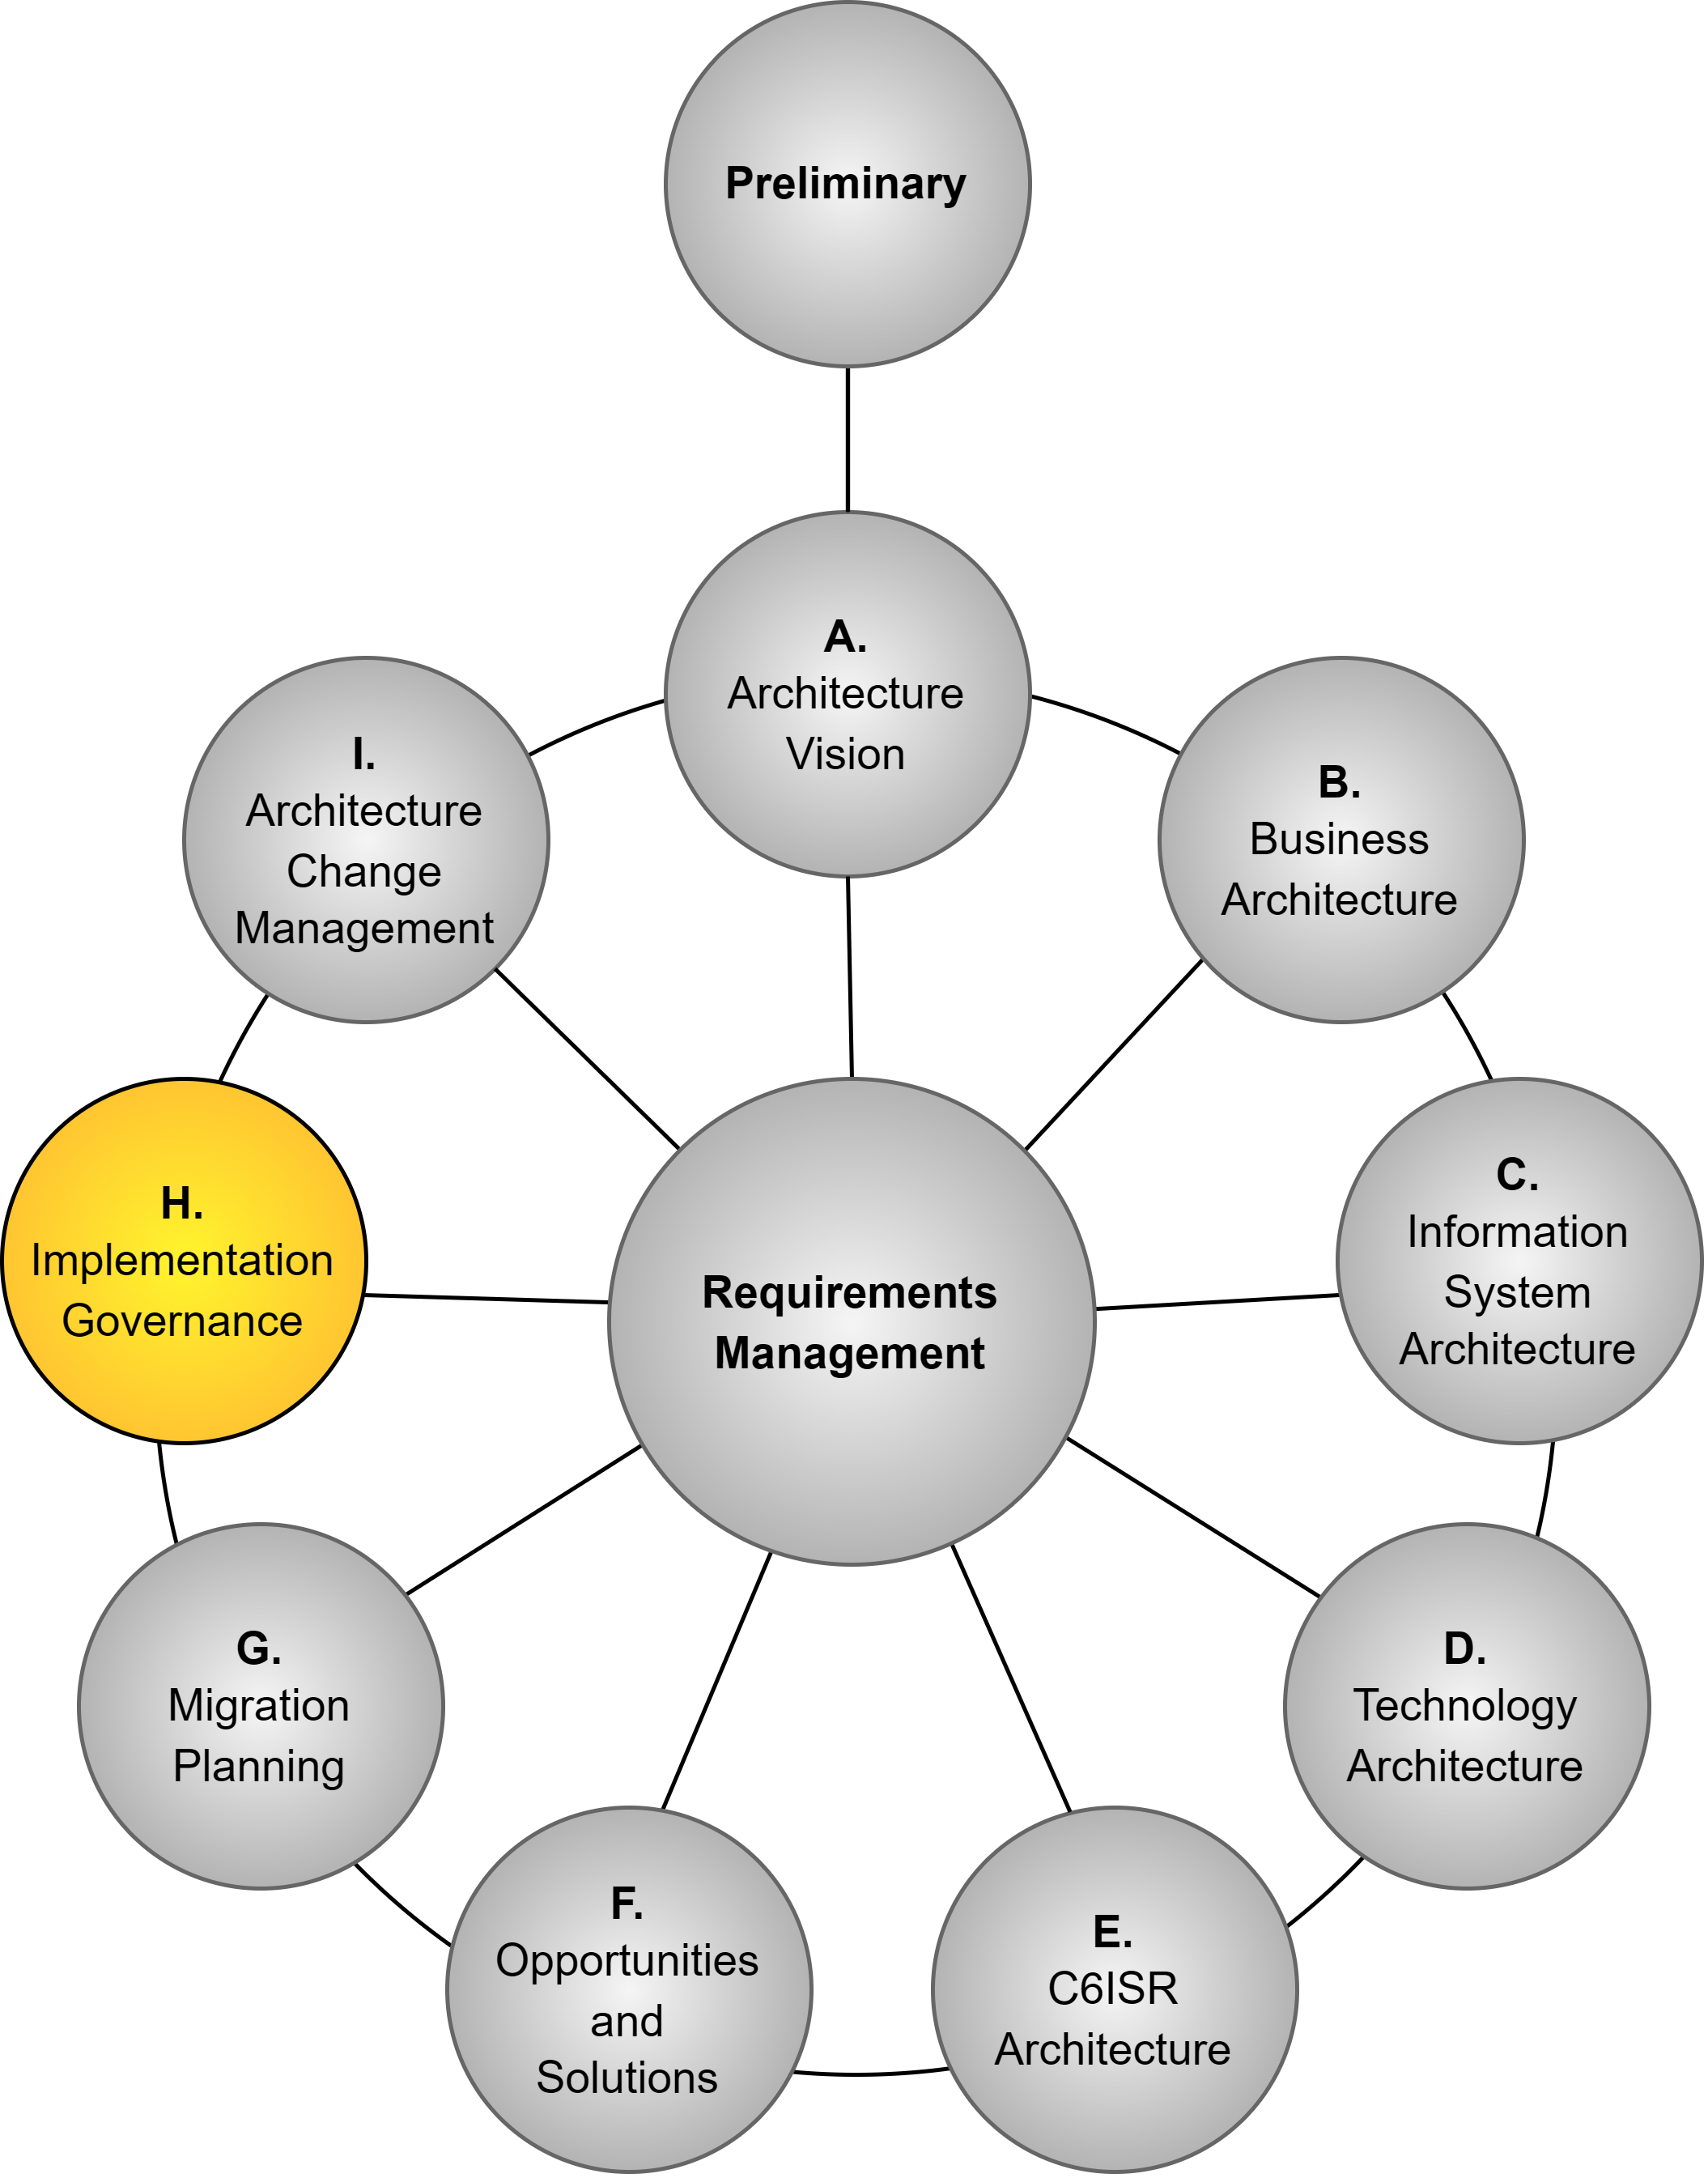
\includegraphics[width=0.46\linewidth,height=0.8\textheight,keepaspectratio]{images/Fase Implementation Governance.drawio.png}
\caption{Fase \textit{Implementation Governance}}
\label{fig:III.12}
\end{figure}

Input, step, dan output Fase Implementation Governance disajikan pada Tabel~\ref{tab:III.16}.

\begingroup\small\setstretch{1.0}
\begin{longtable}{@{}>{\raggedright\arraybackslash\hspace{0pt}}p{0.312\linewidth}>{\raggedright\arraybackslash\hspace{0pt}}p{0.312\linewidth}>{\raggedright\arraybackslash\hspace{0pt}}p{0.312\linewidth}@{}}
\caption{Input, Step, dan Output Fase \textit{Implementation Governance}}\label{tab:III.16}\\
\toprule
\textbf{INPUT} & \textbf{STEP} & \textbf{OUTPUT}\\
\midrule
\endfirsthead
\multicolumn{3}{@{}l}{\small\itshape \tablename\ \thetable{} (lanjutan)}\\
\toprule
\textbf{INPUT} & \textbf{STEP} & \textbf{OUTPUT}\\
\midrule
\endhead
\bottomrule
\endlastfoot
\hangindent=1.1em\hangafter=1 \makebox[1.1em][l]{1.}Rencana implementasi dan migrasi\par \hangindent=1.1em\hangafter=1 \makebox[1.1em][l]{2.}\textit{Architecture Definition Document} dan \textit{Architecture Requirements Specification final}\par \hangindent=1.1em\hangafter=1 \makebox[1.1em][l]{3.}\textit{Roadmap} arsitektur\par \hangindent=1.1em\hangafter=1 \makebox[1.1em][l]{4.}Model tata kelola implementasi dan kontrak arsitektur\par \hangindent=1.1em\hangafter=1 \makebox[1.1em][l]{5.}Prinsip arsitektur dan ketentuan regulasi nasional & \hangindent=1.1em\hangafter=1 \makebox[1.1em][l]{1.}Mengonfirmasi ruang lingkup dan prioritas penggelaran\par \hangindent=1.1em\hangafter=1 \makebox[1.1em][l]{2.}Mengidentifikasi sumber daya dan keahlian pelaksana\par \hangindent=1.1em\hangafter=1 \makebox[1.1em][l]{3.}Memandu pengembangan dan penggelaran solusi\par \hangindent=1.1em\hangafter=1 \makebox[1.1em][l]{4.}Melaksanakan tinjauan kepatuhan terhadap arsitektur, regulasi nasional, dan ketentuan sektor pertahanan\par \hangindent=1.1em\hangafter=1 \makebox[1.1em][l]{5.}Melaksanakan tinjauan pascaimplementasi & \hangindent=1.1em\hangafter=1 \makebox[1.1em][l]{1.}Kontrak arsitektur yang ditandatangani\par \hangindent=1.1em\hangafter=1 \makebox[1.1em][l]{2.}Hasil penilaian kepatuhan\par \hangindent=1.1em\hangafter=1 \makebox[1.1em][l]{3.}Permintaan perubahan\par \hangindent=1.1em\hangafter=1 \makebox[1.1em][l]{4.}Solusi yang patuh terhadap arsitektur\\
\end{longtable}
\endgroup

Keterangan: seluruh muatan mengikuti TOGAF ADM standar.

Tabel~\ref{tab:III.16} menunjukkan bahwa tinjauan kepatuhan menjadi inti fase ini.

\subsection{Fase \textit{Architecture Change Management}}
\label{sec:III.3.10}

Fase Architecture Change Management mengelola perubahan arsitektur secara terkendali sebagai respons terhadap dinamika lingkungan strategis pertahanan, teknologi, dan kebijakan. Fase ini terhubung kembali dengan Fase Architecture Vision sehingga siklus dapat berulang, sebagaimana ditunjukkan pada Gambar~\ref{fig:III.13}.
\begin{figure}[htbp]
\centering
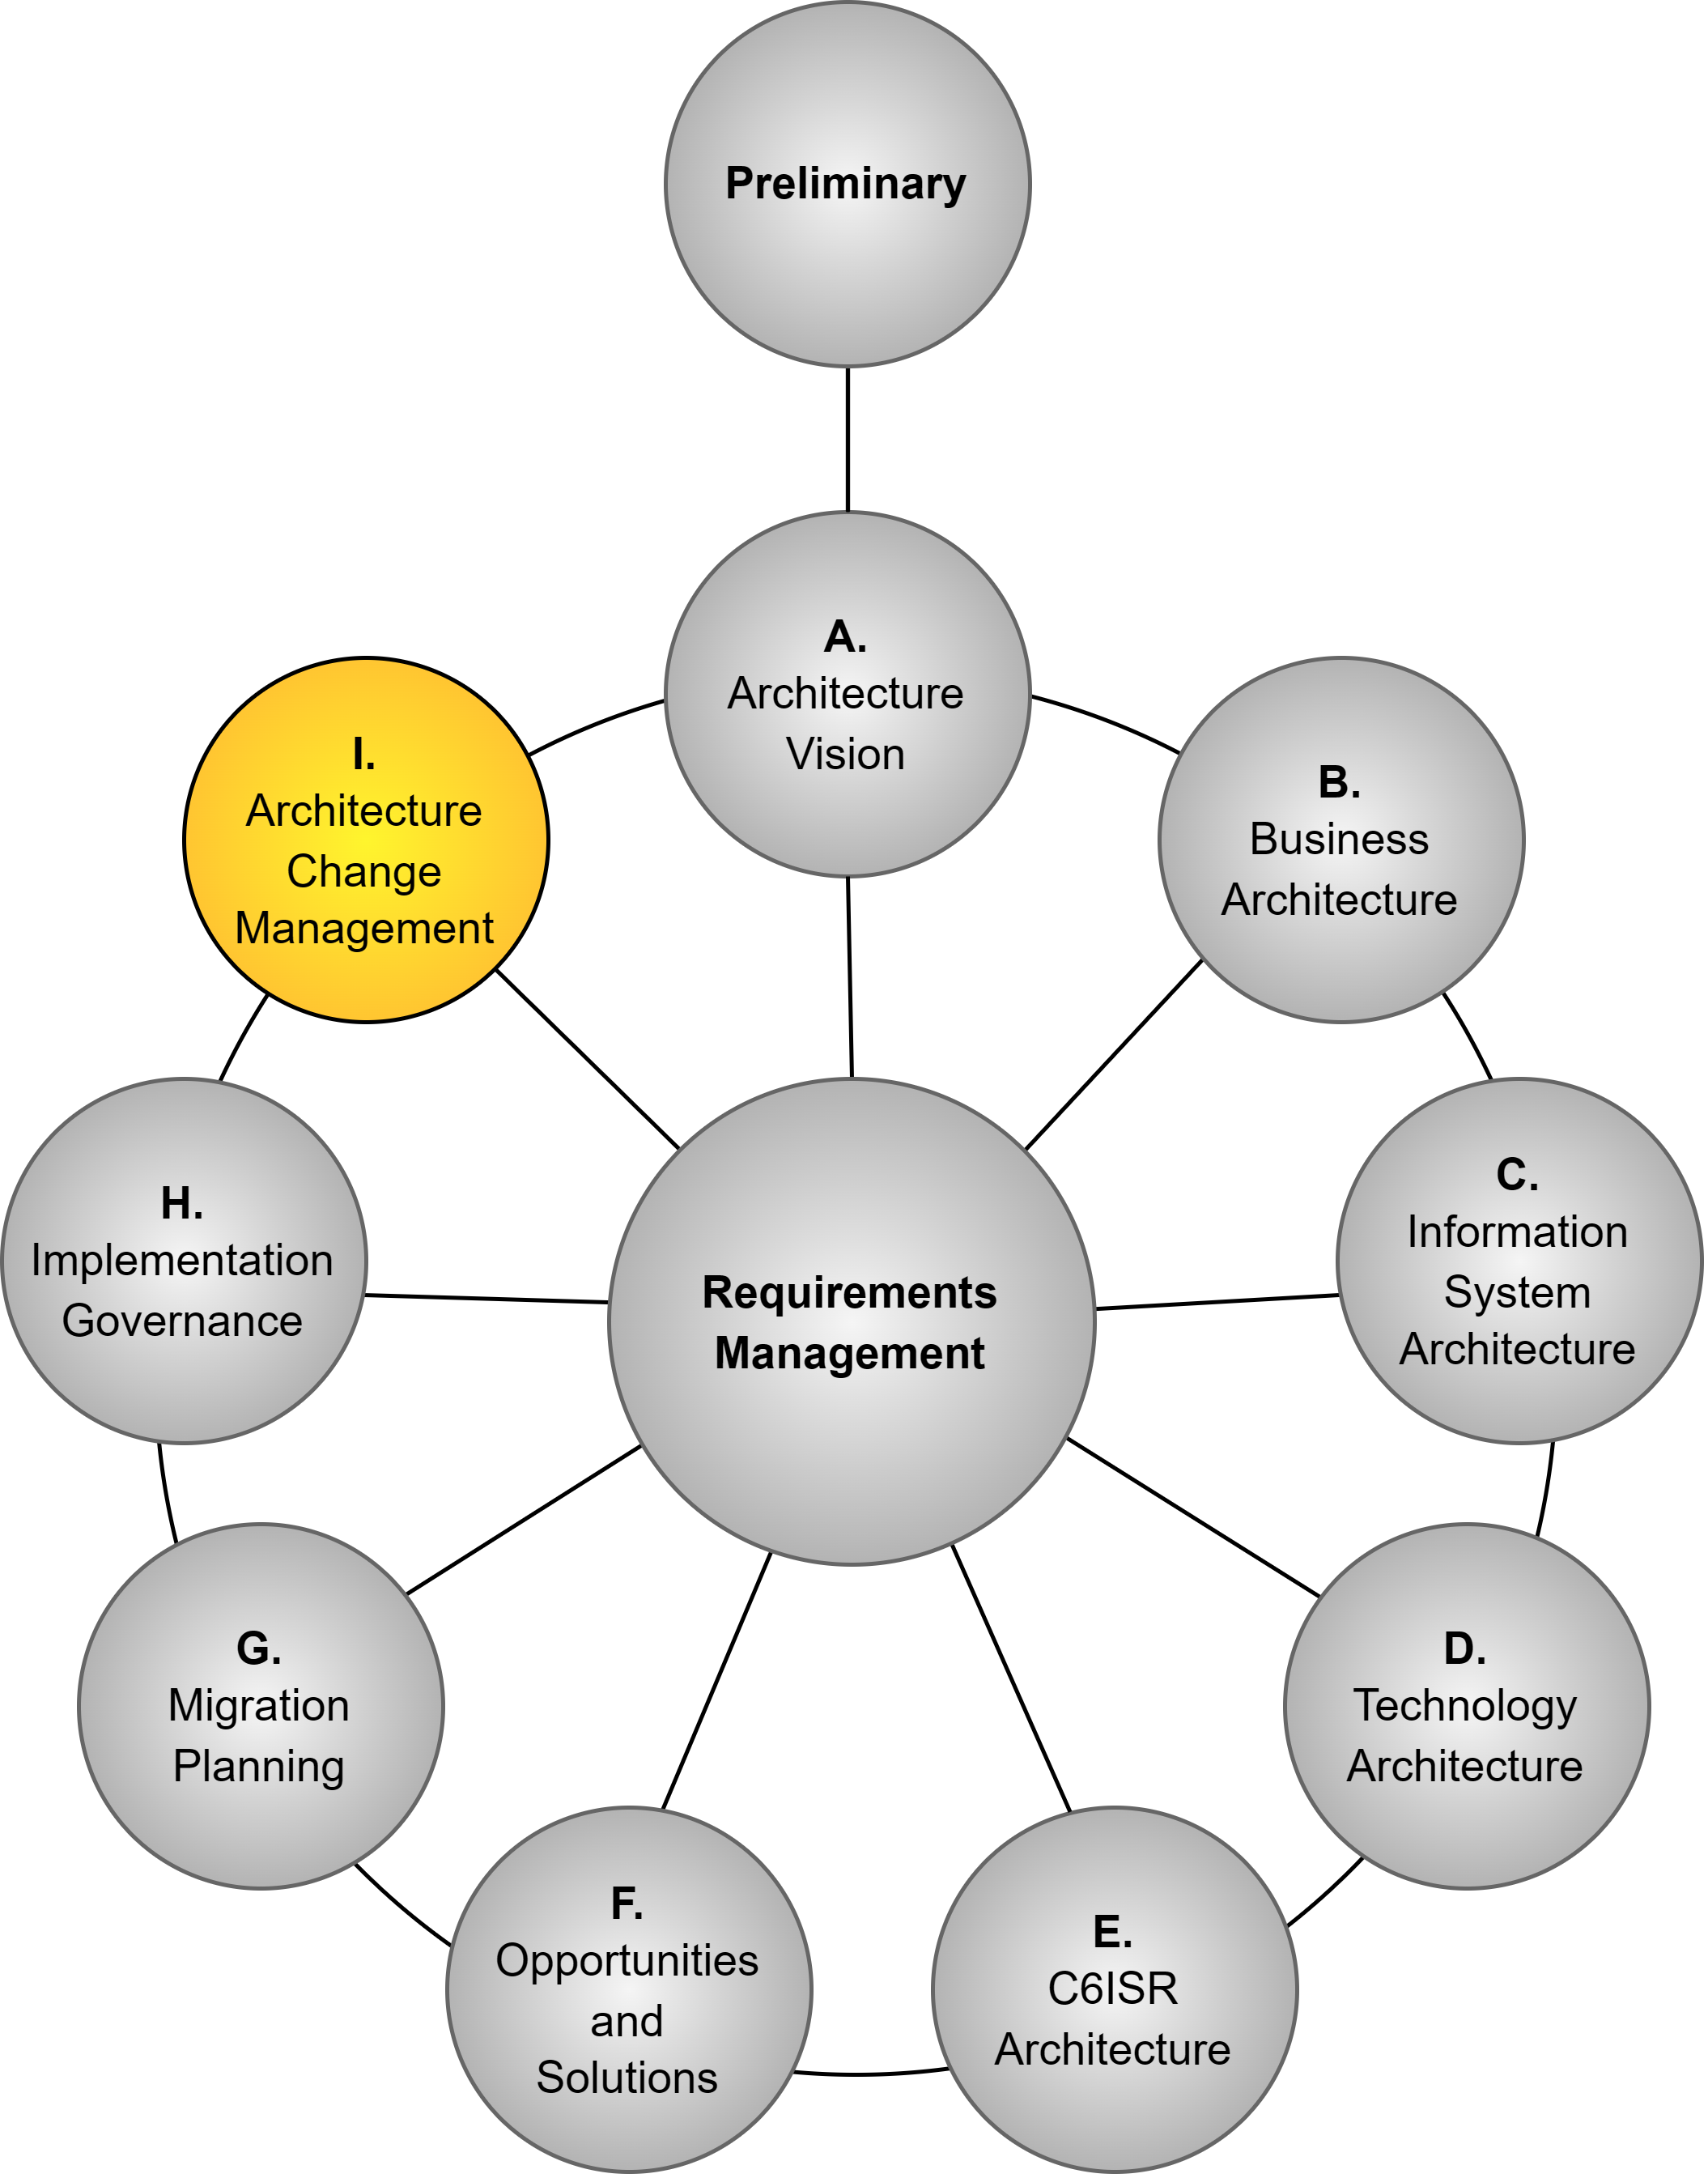
\includegraphics[width=0.46\linewidth,height=0.8\textheight,keepaspectratio]{images/Fase Architecture Change Management.drawio.png}
\caption{Fase \textit{Architecture Change Management}}
\label{fig:III.13}
\end{figure}

Input, step, dan output Fase \textit{Architecture Change Management} disajikan pada Tabel~\ref{tab:III.17}.

\begingroup\small\setstretch{1.0}
\begin{longtable}{@{}>{\raggedright\arraybackslash\hspace{0pt}}p{0.312\linewidth}>{\raggedright\arraybackslash\hspace{0pt}}p{0.312\linewidth}>{\raggedright\arraybackslash\hspace{0pt}}p{0.312\linewidth}@{}}
\caption{Input, Step, dan Output Fase \textit{Architecture Change Management}}\label{tab:III.17}\\
\toprule
\textbf{INPUT} & \textbf{STEP} & \textbf{OUTPUT}\\
\midrule
\endfirsthead
\multicolumn{3}{@{}l}{\small\itshape \tablename\ \thetable{} (lanjutan)}\\
\toprule
\textbf{INPUT} & \textbf{STEP} & \textbf{OUTPUT}\\
\midrule
\endhead
\bottomrule
\endlastfoot
\hangindent=1.1em\hangafter=1 \makebox[1.1em][l]{1.}Hasil implementasi dan umpan balik operasional\par \hangindent=1.1em\hangafter=1 \makebox[1.1em][l]{2.}Kontrak arsitektur dan hasil penilaian kepatuhan\par \hangindent=1.1em\hangafter=1 \makebox[1.1em][l]{3.}\textit{Architecture Definition Document}, \textit{Architecture Requirements Specification}, dan \textit{roadmap} arsitektur\par \hangindent=1.1em\hangafter=1 \makebox[1.1em][l]{4.}Perubahan lingkungan strategis pertahanan, teknologi, dan regulasi & \hangindent=1.1em\hangafter=1 \makebox[1.1em][l]{1.}Menetapkan proses perwujudan nilai\par \hangindent=1.1em\hangafter=1 \makebox[1.1em][l]{2.}Memantau kinerja arsitektur\par \hangindent=1.1em\hangafter=1 \makebox[1.1em][l]{3.}Memantau perubahan lingkungan strategis pertahanan, teknologi, dan regulasi\par \hangindent=1.1em\hangafter=1 \makebox[1.1em][l]{4.}Menilai dampak perubahan\par \hangindent=1.1em\hangafter=1 \makebox[1.1em][l]{5.}Mengelola risiko dan permintaan perubahan\par \hangindent=1.1em\hangafter=1 \makebox[1.1em][l]{6.}Mengaktifkan pelaksanaan perubahan secara terkendali & \hangindent=1.1em\hangafter=1 \makebox[1.1em][l]{1.}Pemutakhiran arsitektur\par \hangindent=1.1em\hangafter=1 \makebox[1.1em][l]{2.}Perubahan pada \textit{framework} dan prinsip arsitektur\par \hangindent=1.1em\hangafter=1 \makebox[1.1em][l]{3.}\textit{Request for Architecture Work} baru\par \hangindent=1.1em\hangafter=1 \makebox[1.1em][l]{4.}\textit{Statement of Architecture Work} dan kontrak arsitektur yang dimutakhirkan\\
\end{longtable}
\endgroup

Keterangan: seluruh muatan mengikuti TOGAF ADM standar.

Tabel~\ref{tab:III.17} menunjukkan bahwa TOGAF Pertahanan Indonesia bersifat terbuka terhadap penyempurnaan. Perubahan lingkungan ancaman dan kebijakan pertahanan dapat memicu siklus baru, termasuk pemutakhiran prinsip dan framework itu sendiri.

\section{Verifikasi Pemenuhan Kebutuhan \textit{Framework}}
\label{sec:III.4}

Verifikasi dilakukan untuk memastikan bahwa kesepuluh kebutuhan pada Tabel~\ref{tab:III.1} telah dipenuhi oleh TOGAF Pertahanan Indonesia. Verifikasi menelusuri setiap kebutuhan ke komponen rancangan yang memenuhinya. Hasil verifikasi disajikan pada Tabel~\ref{tab:III.18}.

\begingroup\small\setstretch{1.0}
\begin{longtable}{@{}>{\raggedright\arraybackslash\hspace{0pt}}p{0.094\linewidth}>{\raggedright\arraybackslash\hspace{0pt}}p{0.213\linewidth}>{\raggedright\arraybackslash\hspace{0pt}}p{0.351\linewidth}>{\raggedright\arraybackslash\hspace{0pt}}p{0.119\linewidth}>{\raggedright\arraybackslash\hspace{0pt}}p{0.100\linewidth}@{}}
\caption{Verifikasi Pemenuhan Kebutuhan oleh TOGAF Pertahanan Indonesia}\label{tab:III.18}\\
\toprule
\textbf{Kode} & \textbf{Kebutuhan} & \textbf{Mekanisme Pemenuhan} & \textbf{Lokasi} & \textbf{Status}\\
\midrule
\endfirsthead
\multicolumn{5}{@{}l}{\small\itshape \tablename\ \thetable{} (lanjutan)}\\
\toprule
\textbf{Kode} & \textbf{Kebutuhan} & \textbf{Mekanisme Pemenuhan} & \textbf{Lokasi} & \textbf{Status}\\
\midrule
\endhead
\bottomrule
\endlastfoot
\centering\arraybackslash KF-01 & Metodologi pengembangan yang preskriptif dan iteratif & Siklus ADM dipertahankan dengan \textit{Requirements Management} di pusat siklus. & \centering\arraybackslash III.2.1 & \centering\arraybackslash T $\rightarrow$ T\\
\centering\arraybackslash KF-02 & Cakupan domain arsitektur inti & Fase B, C, dan D dipertahankan, dengan Fase C diuraikan menjadi \textit{Data Architecture} dan \textit{Application Architecture}. & \centering\arraybackslash III.3.3–III.3.5 & \centering\arraybackslash T $\rightarrow$ T\\
\centering\arraybackslash KF-03 & Akomodasi domain C6ISR & Penambahan Fase C6ISR Architecture (+) yang mengintegrasikan enam lapisan C6ISR, diperkuat prinsip \textit{Integrated Command \& Control}. & \centering\arraybackslash III.2.2;\newline III.3.6 & \centering\arraybackslash TT $\rightarrow$ T\\
\centering\arraybackslash KF-04 & Keamanan siber sejak perancangan & Prinsip \textit{Security by Design}, klasifikasi kerahasiaan dan kendali akses data, lapisan keamanan siber pada Fase D, serta lapisan \textit{cyber-defense} pada Fase E. & \centering\arraybackslash III.2.3; III.3.4–III.3.6 & \centering\arraybackslash TS $\rightarrow$ T\\
\centering\arraybackslash KF-05 & Interoperabilitas lintas entitas & Prinsip \textit{Interoperability}, model interoperabilitas lintas matra pada Fase B, serta integrasi dan pertukaran data lintas matra pada Fase C dan Fase E. & \centering\arraybackslash III.2.3;\newline III.3.3;\newline III.3.4;\newline III.3.6 & \centering\arraybackslash TS $\rightarrow$ T\\
\centering\arraybackslash KF-06 & Keterkaitan dengan doktrin dan strategi pertahanan & Doktrin dan strategi pertahanan menjadi input Fase \textit{Preliminary} dan Fase A, diperkuat prinsip \textit{Smart Defence Oriented}. & \centering\arraybackslash III.2.3;\newline III.3.1;\newline III.3.2 & \centering\arraybackslash TT $\rightarrow$ T\\
\centering\arraybackslash KF-07 & Keselarasan dengan regulasi nasional & Regulasi SPBE, Arsitektur SPBE, dan Satu Data Pertahanan menjadi input Fase \textit{Preliminary}, diperkuat prinsip \textit{Governance \& Compliance}. & \centering\arraybackslash III.2.3;\newline III.3.1 & \centering\arraybackslash T $\rightarrow$ T\\
\centering\arraybackslash KF-08 & Fleksibilitas penyesuaian & Modifikasi bersifat aditif, yaitu satu fase ditambahkan dan lima fase disesuaikan tanpa mengubah struktur ADM. & \centering\arraybackslash III.2.1 & \centering\arraybackslash T $\rightarrow$ T\\
\centering\arraybackslash KF-09 & Tata kelola dan manajemen perubahan arsitektur & Kerangka tata kelola ditetapkan pada Fase \textit{Preliminary}, sedangkan Fase \textit{Implementation Governance} dan \textit{Architecture Change Management} dipertahankan. & \centering\arraybackslash III.3.1;\newline III.3.9;\newline III.3.10 & \centering\arraybackslash T $\rightarrow$ T\\
\centering\arraybackslash KF-10 & Ketersediaan dan kematangan ekosistem & TOGAF tetap menjadi basis sehingga ekosistem pengetahuan dan ketersediaannya tetap dapat dimanfaatkan. & \centering\arraybackslash III.2.1 & \centering\arraybackslash T $\rightarrow$ T\\
\end{longtable}
\endgroup

Keterangan: Status = tingkat pemenuhan oleh TOGAF standar (Tabel~\ref{tab:III.2}) $\rightarrow$ tingkat pemenuhan oleh TOGAF Pertahanan Indonesia.

Tabel~\ref{tab:III.18} menunjukkan bahwa seluruh kebutuhan terpenuhi pada tingkat rancangan. Empat kebutuhan yang sebelumnya belum terpenuhi oleh TOGAF standar dipenuhi melalui satu fase baru, penyesuaian muatan fase, dan prinsip arsitektur, sedangkan kebutuhan yang telah terpenuhi tetap terjaga karena struktur ADM tidak diubah. Verifikasi ini bersifat \textit{ex-ante}. Kelayakan framework selanjutnya diuji melalui penerapan pada Kemhan RI di Bab IV dan evaluasi oleh pakar di Bab V.
